%!TEX root = ../main.tex

%%%%%%%%%%%%%%%%%%%%%%%%%%%%%%%
%%%%%%%%%%%%%%%%%%%%%%%%%%%%%%%
\chapter{Theoretical basics}
\label{chap:theoretical}

This chapter contains an overview of the physical principles on which the experiment is based. Firstly, light-molecule interactions are described in general before the scattering effects that are measured during Raman spectroscopy are considered. The complete chapter is cited from the laboratory script \autocite{brauerApplicationRamanSpectroscopy2022}, standard literature in optics \autocite{bornPrinciplesOpticsElectromagnetic1999,hechtOptik2005,lipsonOptik1997,niedrigOptikWellenUnd2004} and further specifically considering Raman application \autocite{herzbergMolecularSpectraMolecular2013,schraderInfraredRamanSpectroscopy1995}. 

%%%%%%%%%%%%%%%%%%%%%%%%%%%%%%%
\section{Properties of light}

As per the light wave duality, light can be described as both a wave and a massless particle. The energy of light is transported by photons, each of which carries an amount of energy equal to its frequency multiplied by Planck’s quantum of action.
\begin{align}
    E=h \cdot f
\end{align}
By inserting the standard equation for wave propagation, it can be shown that the Energy of a photon is inversely proportional to its wavelength.
\begin{align}
    c&=f \cdot \lambda \\
    E&= \frac{h \cdot c}{\lambda}
\end{align}
The wavenumber $\nu$ is used to quantify the energy of a photon in a simple manner.
\begin{align}
    \nu=\frac{1}{\lambda}
\end{align}

%%%%%%%%%%%%%%%%%%%%%%%%%%%%%%%
\section{Properties of molecules}

Apart from translational energy, which does not influence light-molecule interactions, molecules can occupy a discrete set of energetic states that are characterized by the electronic, vibrational, and rotational quantum numbers $n$, $v$, and $J$ respectively.

\subsection{Electronic energy states}

The largest energy differences can be found between the electronic energy states, which are quantified by the principal quantum number n. A shift in the electronic state is much bigger than the difference between a pair of vibrational levels. The energy gap between two neighboring rotational states is the smallest. \autoref{fig:energy-states} illustrates the distribution of the different energetic states.

\begin{figure}[!htb]
    \centering
    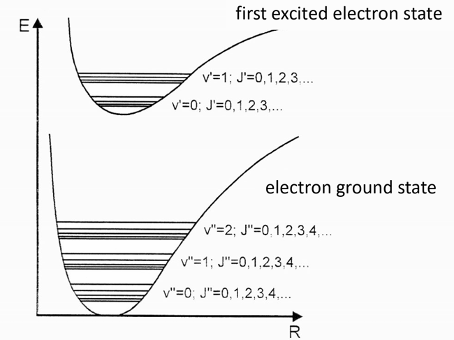
\includegraphics[width=.6\textwidth]{02kapitel/energy-states.png}
    \caption[Potential energy curves with some energy levels]{Potential energy curves of a molecule with some sketched energy levels (vibrational and rotational), scheme after \autocite{brauerApplicationRamanSpectroscopy2022}}
    \label{fig:energy-states}
\end{figure}

Because of the high energies needed visible light can usually not excite a molecule electronically. Because the light source used in the experiment lies within the visible range the effects of electronic excitation will not be discussed any further at this point.

\subsection{Vibrational energy states}

As a molecule consists of multiple interconnected atoms it can perform several types of oscillations. The number of degrees of freedom of a molecule depends on the number of atoms N in the molecule and their positioning relative to each other. While linear molecules have 3N-5 degrees of freedom, non-linear molecules can oscillate with 3N-6 degrees of freedom. \autoref{fig:vib-states} shows the several types of oscillation for a diatomic molecule (Hydrogen) as well as linear and non-linear three atomic molecules using the examples of carbon dioxide and water, respectively.

\begin{figure}[!htb]
    \centering
    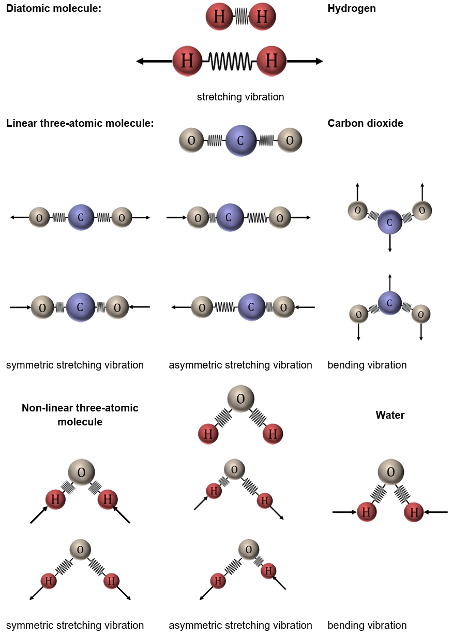
\includegraphics[width=.7\textwidth]{02kapitel/vib-states.png}
    \caption[Normal modes of selected molecules]{Normal vibrational modes of molecules; water ($\mathrm{H_2O}$) and $\mathrm{CO_2}$ \autocite{brauerApplicationRamanSpectroscopy2022}}
    \label{fig:vib-states}
\end{figure}

It should also be noted that the vibration of a molecule is best described by the model of an anharmonic oscillator, due to the binding forces between the atoms diminishing as their distance increases. This effect dampens the vibration of the molecule which is why a harmonic oscillator does not allow for an accurate description of the energy levels. The dampening also leads to a diminishing energy difference between neighboring energy levels as the vibrational quantum number $\nu$ increases. In \autoref{fig:anharmonic-osz} both models are compared.

\begin{figure}[!htb]
    \centering
    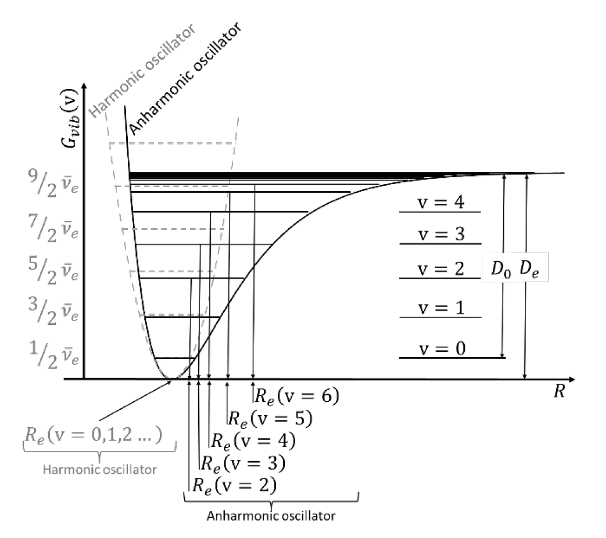
\includegraphics[width=.7\textwidth]{02kapitel/anharmonic-osz.png}
    \caption[Model of an anharmonic oszillator]{Harmonic and anharmonic potential curves with the corresponding energy level diagram
    of the oscillation states \autocite{brauerApplicationRamanSpectroscopy2022}}
    \label{fig:anharmonic-osz}
\end{figure}

\subsection{Rotational energy states}

The smallest energetic differences can be found in the rotational stage. The rotational energy of a molecule is quantified by the rotational quantum number $J$. A simple model to describe the rotational energy of the molecule is the rigid rotator, which consists of two mass points with a fixed distance between them. \autoref{eq:rigid-rotator} shows how the rotational states would be quantified for a rigid rotator with $I_\mathrm{e}$ being the molecule moment of inertia and $B_\mathrm{e}$ being the rotational constant.
\begin{align}
    F(J)&=\frac{E_\mathrm{rot}(J)}{h \cdot c}=\frac{h}{8\pi^2 \cdot c \cdot I_\mathrm{e}} \cdot J \cdot (J+1) \nonumber \\[6pt]
    F(J)&=B_\mathrm{e} \cdot J \cdot (J+1) \label{eq:rigid-rotator}
\end{align}
In reality, however, the atoms of a molecule are connected by a force of attraction rather than a fixed distance.  Due to vibrations or in this case centrifugal forces, the distance between the atoms will change. Therefore, molecules are non-rigid rotators, which leads to the energy levels being lower than they would be for a rigid rotator as is illustrated in \autoref{fig:rot-states}.

\begin{figure}[!htb]
    \centering
    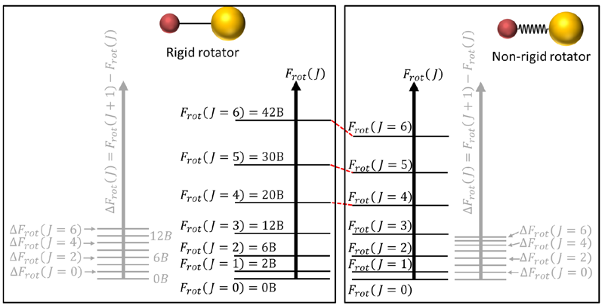
\includegraphics[width=.8\textwidth]{02kapitel/rot-states.png}
    \caption[Scheme of rotational energy states: Rigid vs. Non-rigid rotator]{Schematic diagram of a rigid and a non-rigid rotator and the corresponding rotational energy levels \autocite{brauerApplicationRamanSpectroscopy2022}}
    \label{fig:rot-states}
\end{figure}

%%%%%%%%%%%%%%%%%%%%%%%%%%%%%%%
\section{Photon-molecule interactions}

Because of the discrete nature of the energetic states of molecules, different kinds of interactions between photons and molecules can be observed.

\subsection{Flourescence}

\begin{wrapfigure}{R}{.5\textwidth}
    \setcapwidth[c]{.8\linewidth}
    \centering
    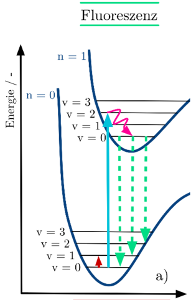
\includegraphics[width=.3\textwidth]{02kapitel/flourescence.png}
    \caption[Energy scheme of flourescence]{Potential energy curve with scheme of fluorescence processes \autocite{brauerApplicationRamanSpectroscopy2022}}
    \label{fig:flourescence}
\end{wrapfigure}
Photons carrying a sufficient amount of energy may excite molecules into a higher electronic state. Relaxation processes lead to the molecule falling into a lower vibrational state, still within the excited electronic state. From there another fallback occurs which takes the molecule back to the electronic ground state. As the molecule may end up in different vibrational states after the fallback, fluorescence releases photons of different energies and thus emits a broad spectrum of light. \autoref{fig:flourescence} presents the process of fluorescence in a schematic manner where the dotted arrows indicate the emission of different wavelengths. The energy of infrared and visible light is not enough to induce fluorescence usually.

\subsection{Infrared absorption}

When the energy of a photon matches exactly with the difference between the current and any higher energetic state of a molecule, it is absorbed. As the photons of infrared light carry relatively low amounts of energy the molecule cannot be promoted into a higher electronic state, which means that in contrast to fluorescence, no fallback occurs and thus no photon is emitted. After the absorption, the photon no longer exists as its entire energy has been used to transfer the molecule into a higher energetic state. Instead of emitting a photon during relaxation, the surplus of energy is dissipated into the environment through heat. As the distribution of energetic states is characteristic of each molecule, absorption spectroscopy can be used to identify which molecules are present in a sample.

\subsection{Scattering effects}

If the energy of a photon does not match any energy gap inside the molecule, the photon will be scattered. In contrast to absorption, the photon does not cease to exist as it is only redirected in a random direction away from the molecule it collided with. Scattering effects can be categorized into elastic and inelastic scattering. Elastic scattering describes scattering processes where no energy is transferred and is also known as Rayleigh-Scattering. In the case of inelastic scattering, energy has been transferred between the photon and the molecule.

\begin{figure}[!htb]
    \centering
    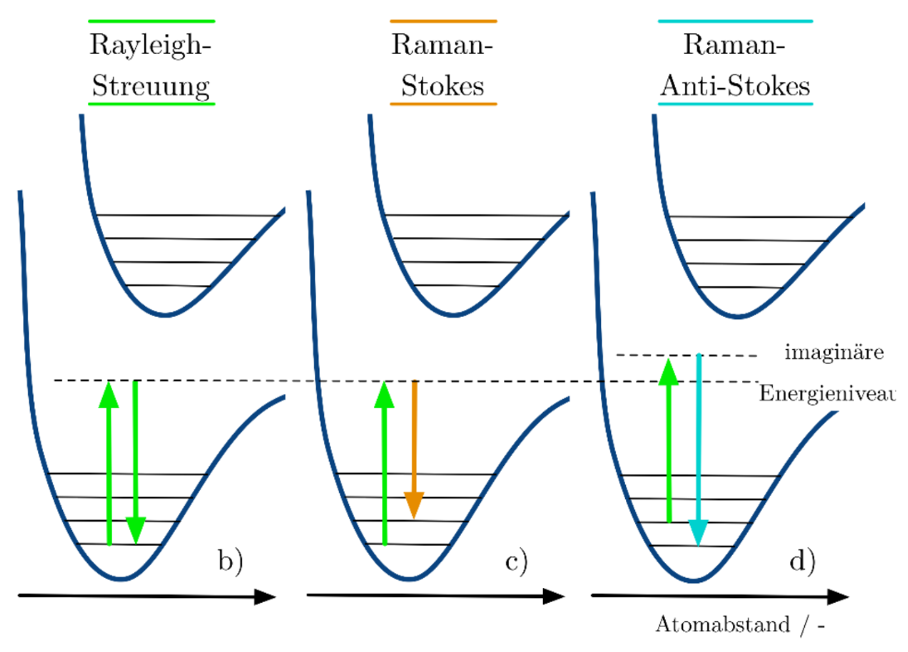
\includegraphics[width=.8\textwidth]{02kapitel/scattering.png}
    \caption[Energy diagrams of scattering events]{Different ways of interaction of photon and molecule: b) Rayleigh scattering; c) Raman-Stokes transition; d) Raman-Anti-Stokes transition \autocite{brauerApplicationRamanSpectroscopy2022}}
    \label{fig:scattering}
\end{figure}

Depending on whether energy was transferred from the photon to the molecule or vice versa, inelastic scattering can be divided into Raman-Stokes and Raman-Anti-Stokes scattering. During Raman-Stokes scattering the photon transfers energy to the molecule which results in a lower energy and therefore red-shifted photon being scattered and the molecule residing in a higher energetic state than before. Raman-Anti-Stokes scattering on the other hand leads to a higher energy, blue shifted photon being scattered and leaves the molecule on a lower energetic level. Thus Raman-Anti-Stokes scattering cannot occur with the molecule beginning in the ground state as it cannot release any more energy. Consequently, Raman-Anti-Stokes is less prevalent than Raman-Stokes scattering because the number of molecules in lower energetic states is always higher than the number of molecules residing in higher energetic states, which is described by the Boltzmann distribution. \autoref{fig:scattering} illustrates the energetic transitions of scattering processes.

The energy difference between incoming and outgoing photons is quantified by the so-called Raman shift, which is expressed as a wavenumber. By analyzing the signal intensity at certain wavenumbers, conclusions can be drawn about the molecular composition and temperature of a sample.

%%%%%%%%%%%%%%%%%%%%%%%%%%%%%%%
%%%%%%%%%%%%%%%%%%%%%%%%%%%%%%%
\chapter{Experimental setup}
\label{chap:experimental}

A correct interpretation of empirical data requires knowledge of the experimental setup. This chapter contains a description of the physical apparatus used in the experiment as well as the measurement procedure.

%%%%%%%%%%%%%%%%%%%%%%%%%%%%%%%
\section{Measurement setup and preparations}

In this experiment, a diode-pumped, frequency-doubled continuous wave laser is used as the excitation light source. It emits light with a power of $250~\mathrm{mW}$ and a wavelength of $532~\mathrm{nm}$. A plano-convex lens focuses the laser beam into an optical fibre which directs the light into the Raman measurement head. Inside the measurement head, the optical fibre is followed by a convex lens which is used to collimate the light before it passes through a laser line filter. A dichroic beam splitter then reflects the collimated and filtered beam. The beam splitter transmits light with wavelengths higher than $532~\mathrm{nm}$ and reflects shorter-wavelength light. Hence, the incident laser light is reflected in such a way that it leaves the measurement head through a plano-convex lens with a focal length of $150~\mathrm{mm}$. The sample is positioned so that the focal point is inside the measurement volume.

\begin{figure}[!htb]
    \centering
    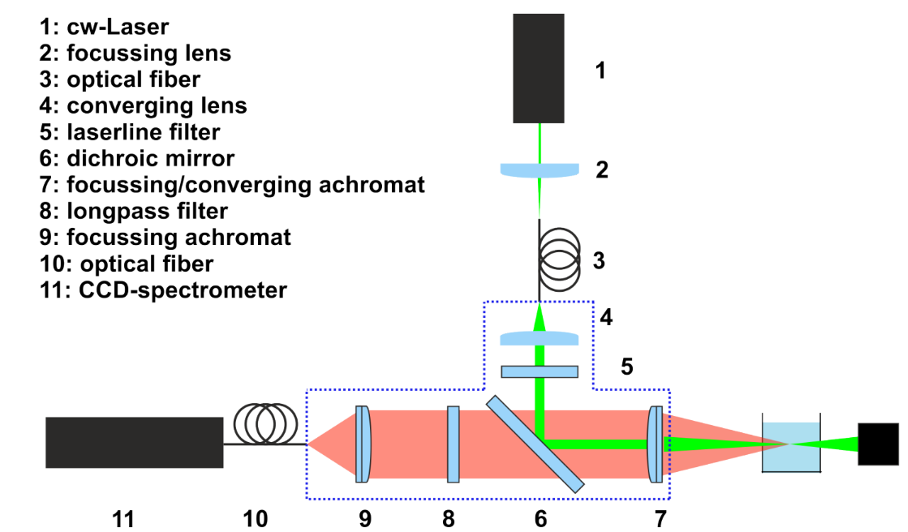
\includegraphics[width=.8\textwidth]{02kapitel/raman-gun.png}
    \caption[Optical setup for Raman spectroscopy measurements]{Optical setup for Raman spectroscopy measurements \autocite{brauerApplicationRamanSpectroscopy2022}}
    \label{fig:raman-gun}
\end{figure}

The light scattered in the measurement volume is detected in backscatter, where the lens focusing the laser beam also collects and aligns the scattered light. The dichroic beam splitter reflects the elastically scattered Rayleigh signal ($\lambda = 532 \mathrm{nm}$) and transmits the inelastically scattered Raman signal ($\lambda > 532 \mathrm{nm}$). To eliminate the remaining Rayleigh signal, a long-pass filter (8, RazorEdge\textsuperscript{\textcopyright} filter) with a cutoff at $532~\mathrm{nm}$ is used. A $100~\mathrm{mm}$ focal length lens (9) precisely focuses the signal into the center of the optical fiber bundle, guiding it to the spectrometer. Within the spectrometer, the signal is projected onto a CCD chip with 1044 pixels, resolving the wavelength range from $535.04~\mathrm{nm}$ to $705.84~\mathrm{nm}$.

%%%%%%%%%%%%%%%%%%%%%%%%%%%%%%%
\section{Execution}

\subsection{Determination of the alcohol content of an unknown liquid}

To establish a correlation between Raman signal intensities and ethanol concentrations, calibration measurements are performed with known concentrations. The following molar fractions of ethanol are used for calibration:
\begin{align}
    x_\mathrm{EtOH}=\{0.0; 0.1; 0.2; 0.4; 0.6; 0.8; 1.0\} \nonumber
\end{align}
Guided by specified densities and molar masses, a consistent total volume of $20~\mathrm{ml}$ is maintained for each solution. Volumes were precalculated, as depicted in \autoref{tab:ethanol-conc} and the measurements are conducted at room temperature.

\begin{table}[!htb]
    \centering
    \small
    \caption[Pre-calculation of volumes and volume fractions]{Pre-calculation of volumes and volume fractions for the experiment; table is showing in-between results as well}
    \label{tab:ethanol-conc}
    \vspace{12pt}
    \begin{tabularx}{\textwidth}{|l|l|l|l|l|l|X|}
        \hline 
        \rowcolor{lightgray} $x_\mathrm{EtOH}$ & $n_\mathrm{EtOH}~\mathrm{[mol]}$ & $n_\mathrm{H_2O}~\mathrm{[mol]}$ & $V_\mathrm{EtOH}~\mathrm{[m^3]}$ & $V_\mathrm{H_2O}~\mathrm{[m^3]}$ & $V_\mathrm{control}~\mathrm{[ml]}$ & Volume fraction $\mathrm{EtOH}$ \\ \hline \hline
        1	& 0,34 & 	0,00 & 	0,0000200 & 	0,0000000 & 	20,00 & 	1,00  \\ \hline
        0,8	& 0,32 & 	0,08 & 	0,0000186 & 	0,0000014 & 	20,00 & 	0,93  \\ \hline
        0,6	& 0,28 & 	0,19 & 	0,0000166 & 	0,0000034 & 	20,00 & 	0,83  \\ \hline
        0,4	& 0,23 & 	0,35 & 	0,0000137 & 	0,0000063 & 	20,00 & 	0,68  \\ \hline
        0,2	& 0,15 & 	0,61 & 	0,0000090 & 	0,0000110 & 	20,00 & 	0,45  \\ \hline
        0,1	& 0,09 & 	0,82 & 	0,0000053 & 	0,0000147 & 	20,00 & 	0,27  \\ \hline
        0	& 0,00 & 	--	 &  0,0000000 &  	0,0000200 &  	20,00 &  	0,00  \\ \hline

    \end{tabularx}
\end{table}

\begin{align}
    V_\mathrm{ges}&=\frac{n_\mathrm{EtOH} \cdot M_\mathrm{EtOH}}{\rho_\mathrm{EtOH}} + \frac{n_\mathrm{H_2O} \cdot M_\mathrm{H_2O}}{\rho_\mathrm{H_2O}} \\[6pt]
    n_\mathrm{H_2O}&=\frac{n_\mathrm{EtOH} \cdot (1-x_\mathrm{EtOH})}{x_\mathrm{EtOH}} \\[6pt]
    V&=\frac{n \cdot M}{\rho}
\end{align}

The measurements are conducted in the software "SpectraSuite". Exposure time is set to $1~\mathrm{s}$, before recording and subtracting a dark spectrum, and optimizing the cuvette's position in the laser beam. Ten Raman spectra are captured, saved, and exported for each mixture. After room lighting was restored, subsequent steps included sample replacement, process repetition, and saving spectra for different compositions in the designated folder. At last, the spectrum of the cuvette containing the unknown mixture is recorded.

\subsection{Measurement of the temperature}

For observing the temperature of a liquid, the experimental setup of \autoref{fig:raman-temp-setup} is used. It contains a bigger glass cuvette, the liquid, a stirring fish and a type-K thermocouple for externally measuring the temperature as validation resp. comparison. With this setup, a homogeneous mixture shall be obtained. Under the cuvette, a heating plate is placed, which is also used to rotate the (magnetic) mixer. The laser beam must not meet with the thermocouple or the stirring fish.

\begin{figure}[!htb]
    \centering
    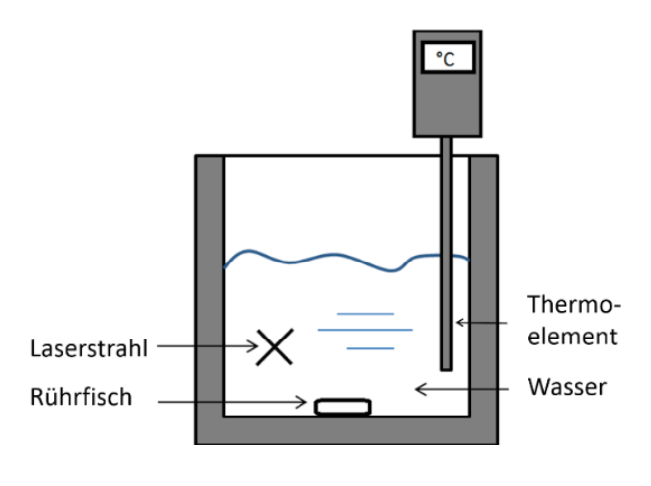
\includegraphics[width=.6\textwidth]{02kapitel/temp-raman.png}
    \caption[Additional measurement setup for temperature determination with Raman]{Additional measurement setup for temperature determination with Raman \autocite{brauerApplicationRamanSpectroscopy2022}}
    \label{fig:raman-temp-setup}
\end{figure}

The beaker is initially filled with $100~\mathrm{ml}$ of water and the stirring plate is set to level three. The room light is turned off, and the integration time of the CCD is set to $1~\mathrm{s}$. After switching on the measurement of the Raman signal and the thermocouple temperature (log every $10~\mathrm{s}$), the heating plate starts heating to $70~\mathrm{^\circ C}$. The heating plate is switched off after $1.5~\mathrm{min}$ $20~\mathrm{ml}$ and water is added. Waiting for another $1.5~\mathrm{min}$, another $20~\mathrm{ml}$ of water is slowly dripped in. After waiting another short time, the beaker is filled with water. The measurement is finished.

%%%%%%%%%%%%%%%%%%%%%%%%%%%%%%%
\section{Evaluation strategy}

\subsection{Determination of the alcohol content of an unknown liquid}

To establish a correlation between the signal intensities and the concentrations of ethanol and water, the separation wavenumber between the two peaks is determined by a combination of graphical and statistical methods. The measured counts $k$ are then accumulated over the spectral bands of each species to determine the overall signal intensities of ethanol and water, respectively.
\begin{align}
    I_\mathrm{EtOH}&=\sum_{2600~\mathrm{cm^{-1}}}^{\nu_\mathrm{separation}} k \\[12pt]
    I_\mathrm{H_2O}&=\sum_{\nu_\mathrm{separation}}^{3800~\mathrm{cm^{-1}}} k
\end{align}
Subsequently, the intensity ratio $r_\mathrm{EtOH}$, which shall be correlated to the molar fraction of ethanol $x_\mathrm{EtOH}$, can be calculated.
\begin{align}
    r_\mathrm{EtOH}=\frac{I_\mathrm{EtOH}}{I_\mathrm{EtOH}+I_\mathrm{H_2O}}
\end{align}
This is done for the results of each of the known mixtures. The calculated intensity ratios are then fitted to the known molar fractions of the mixtures by performing a linear regression. The function of the regression is used to calculate the molar fraction corresponding to the signal intensity of the unknown mixture. At last, the volumetric concentration of ethanol $x_\mathrm{V,EtOH}$ in the unknown mixture is computed using the following formula.
\begin{align}
    x_\mathrm{V,EtOH}=\frac{M_\mathrm{EtOH}}{\rho_\mathrm{EtOH}} \cdot \bigg[ \frac{M_\mathrm{EtOH}}{\rho_\mathrm{EtOH}} + \frac{(1-x_\mathrm{EtOH}) \cdot M_\mathrm{H_2O}}{x_\mathrm{EtOH} \cdot \rho_\mathrm{H_2O}} \bigg]^{-1}
\end{align}

\subsection{Measurement of the temperature}

The data processing of temperature curves and data is rather short. The spectra have to be area-normalized to make them comparable over the curve area ratios. This is realized by dividing each spectral measured intensity through the sum of all data points (equivalent to the integral, due to the integrating CCD behavior). The limits are set to
\begin{align}
    A_\mathrm{left}&= [2600~\mathrm{cm^{-1}},~\Delta \tilde{v}_\mathrm{isosbestic}]\nonumber \\
    A_\mathrm{right}&= [\Delta \tilde{v}_\mathrm{isosbestic},~3800~\mathrm{cm^{-1}}]\nonumber .
\end{align}
The middle limit, the isosbestic point, is calculated from the minimum of the standard deviation of all the recorded area-normalized temperature spectra. This procedure is similar to \autoref{subsec:spec-eval}. The ratio of $A_\mathrm{right}$ to $A_\mathrm{left}$ is then calculated. Inserting this ratio into a polynomial fitted temperature calibration curve\footnote{given from the supervisor}, the temperature of the liquid can be observed. This can then be compared to the measured temperature from the thermocouple K. For comparison, a temperature over time plot with the measurement from both thermocouple and Raman, in addition to the mean error and the mean squared error are useful.

%%%%%%%%%%%%%%%%%%%%%%%%%%%%%%%
%%%%%%%%%%%%%%%%%%%%%%%%%%%%%%%
\chapter{Results}
\label{chap:results}

In this chapter, the data acquired during the experiment is briefly presented and evaluated according to the respective task. The raw data of both experiments can be found in the Excel files submitted with this work.

%%%%%%%%%%%%%%%%%%%%%%%%%%%%%%%
\section{Data presentation and preparation}

\subsection*{Species determination}
\label{subsec:spec-prep}

As per the assignment, the signal intensities are to be accumulated in the range from $2600$ to $3800 \mathrm{cm^{-1}}$. The cut-off wavenumber separates the ethanol from the water peak. Plotting all measured spectra in a single diagram (e.g. \autoref{fig:spectra}), it appears that this separation lies between $3000$ and $3100 \mathrm{cm^{-1}}$.

\begin{figure}[!htb]
    \centering
    %% Creator: Matplotlib, PGF backend
%%
%% To include the figure in your LaTeX document, write
%%   \input{<filename>.pgf}
%%
%% Make sure the required packages are loaded in your preamble
%%   \usepackage{pgf}
%%
%% Also ensure that all the required font packages are loaded; for instance,
%% the lmodern package is sometimes necessary when using math font.
%%   \usepackage{lmodern}
%%
%% Figures using additional raster images can only be included by \input if
%% they are in the same directory as the main LaTeX file. For loading figures
%% from other directories you can use the `import` package
%%   \usepackage{import}
%%
%% and then include the figures with
%%   \import{<path to file>}{<filename>.pgf}
%%
%% Matplotlib used the following preamble
%%   
%%   \usepackage{fontspec}
%%   \setmainfont{Charter.ttc}[Path=\detokenize{/System/Library/Fonts/Supplemental/}]
%%   \setsansfont{DejaVuSans.ttf}[Path=\detokenize{/opt/homebrew/lib/python3.10/site-packages/matplotlib/mpl-data/fonts/ttf/}]
%%   \setmonofont{DejaVuSansMono.ttf}[Path=\detokenize{/opt/homebrew/lib/python3.10/site-packages/matplotlib/mpl-data/fonts/ttf/}]
%%   \makeatletter\@ifpackageloaded{underscore}{}{\usepackage[strings]{underscore}}\makeatother
%%
\begingroup%
\makeatletter%
\begin{pgfpicture}%
\pgfpathrectangle{\pgfpointorigin}{\pgfqpoint{6.400000in}{4.800000in}}%
\pgfusepath{use as bounding box, clip}%
\begin{pgfscope}%
\pgfsetbuttcap%
\pgfsetmiterjoin%
\definecolor{currentfill}{rgb}{1.000000,1.000000,1.000000}%
\pgfsetfillcolor{currentfill}%
\pgfsetlinewidth{0.000000pt}%
\definecolor{currentstroke}{rgb}{1.000000,1.000000,1.000000}%
\pgfsetstrokecolor{currentstroke}%
\pgfsetdash{}{0pt}%
\pgfpathmoveto{\pgfqpoint{0.000000in}{0.000000in}}%
\pgfpathlineto{\pgfqpoint{6.400000in}{0.000000in}}%
\pgfpathlineto{\pgfqpoint{6.400000in}{4.800000in}}%
\pgfpathlineto{\pgfqpoint{0.000000in}{4.800000in}}%
\pgfpathlineto{\pgfqpoint{0.000000in}{0.000000in}}%
\pgfpathclose%
\pgfusepath{fill}%
\end{pgfscope}%
\begin{pgfscope}%
\pgfsetbuttcap%
\pgfsetmiterjoin%
\definecolor{currentfill}{rgb}{1.000000,1.000000,1.000000}%
\pgfsetfillcolor{currentfill}%
\pgfsetlinewidth{0.000000pt}%
\definecolor{currentstroke}{rgb}{0.000000,0.000000,0.000000}%
\pgfsetstrokecolor{currentstroke}%
\pgfsetstrokeopacity{0.000000}%
\pgfsetdash{}{0pt}%
\pgfpathmoveto{\pgfqpoint{0.800000in}{0.528000in}}%
\pgfpathlineto{\pgfqpoint{5.760000in}{0.528000in}}%
\pgfpathlineto{\pgfqpoint{5.760000in}{4.224000in}}%
\pgfpathlineto{\pgfqpoint{0.800000in}{4.224000in}}%
\pgfpathlineto{\pgfqpoint{0.800000in}{0.528000in}}%
\pgfpathclose%
\pgfusepath{fill}%
\end{pgfscope}%
\begin{pgfscope}%
\pgfpathrectangle{\pgfqpoint{0.800000in}{0.528000in}}{\pgfqpoint{4.960000in}{3.696000in}}%
\pgfusepath{clip}%
\pgfsetrectcap%
\pgfsetroundjoin%
\pgfsetlinewidth{0.803000pt}%
\definecolor{currentstroke}{rgb}{0.690196,0.690196,0.690196}%
\pgfsetstrokecolor{currentstroke}%
\pgfsetdash{}{0pt}%
\pgfpathmoveto{\pgfqpoint{1.031213in}{0.528000in}}%
\pgfpathlineto{\pgfqpoint{1.031213in}{4.224000in}}%
\pgfusepath{stroke}%
\end{pgfscope}%
\begin{pgfscope}%
\pgfsetbuttcap%
\pgfsetroundjoin%
\definecolor{currentfill}{rgb}{0.000000,0.000000,0.000000}%
\pgfsetfillcolor{currentfill}%
\pgfsetlinewidth{0.803000pt}%
\definecolor{currentstroke}{rgb}{0.000000,0.000000,0.000000}%
\pgfsetstrokecolor{currentstroke}%
\pgfsetdash{}{0pt}%
\pgfsys@defobject{currentmarker}{\pgfqpoint{0.000000in}{-0.048611in}}{\pgfqpoint{0.000000in}{0.000000in}}{%
\pgfpathmoveto{\pgfqpoint{0.000000in}{0.000000in}}%
\pgfpathlineto{\pgfqpoint{0.000000in}{-0.048611in}}%
\pgfusepath{stroke,fill}%
}%
\begin{pgfscope}%
\pgfsys@transformshift{1.031213in}{0.528000in}%
\pgfsys@useobject{currentmarker}{}%
\end{pgfscope}%
\end{pgfscope}%
\begin{pgfscope}%
\definecolor{textcolor}{rgb}{0.000000,0.000000,0.000000}%
\pgfsetstrokecolor{textcolor}%
\pgfsetfillcolor{textcolor}%
\pgftext[x=1.031213in,y=0.430778in,,top]{\color{textcolor}\rmfamily\fontsize{12.000000}{14.400000}\selectfont \(\displaystyle {2600}\)}%
\end{pgfscope}%
\begin{pgfscope}%
\pgfpathrectangle{\pgfqpoint{0.800000in}{0.528000in}}{\pgfqpoint{4.960000in}{3.696000in}}%
\pgfusepath{clip}%
\pgfsetrectcap%
\pgfsetroundjoin%
\pgfsetlinewidth{0.803000pt}%
\definecolor{currentstroke}{rgb}{0.690196,0.690196,0.690196}%
\pgfsetstrokecolor{currentstroke}%
\pgfsetdash{}{0pt}%
\pgfpathmoveto{\pgfqpoint{1.780650in}{0.528000in}}%
\pgfpathlineto{\pgfqpoint{1.780650in}{4.224000in}}%
\pgfusepath{stroke}%
\end{pgfscope}%
\begin{pgfscope}%
\pgfsetbuttcap%
\pgfsetroundjoin%
\definecolor{currentfill}{rgb}{0.000000,0.000000,0.000000}%
\pgfsetfillcolor{currentfill}%
\pgfsetlinewidth{0.803000pt}%
\definecolor{currentstroke}{rgb}{0.000000,0.000000,0.000000}%
\pgfsetstrokecolor{currentstroke}%
\pgfsetdash{}{0pt}%
\pgfsys@defobject{currentmarker}{\pgfqpoint{0.000000in}{-0.048611in}}{\pgfqpoint{0.000000in}{0.000000in}}{%
\pgfpathmoveto{\pgfqpoint{0.000000in}{0.000000in}}%
\pgfpathlineto{\pgfqpoint{0.000000in}{-0.048611in}}%
\pgfusepath{stroke,fill}%
}%
\begin{pgfscope}%
\pgfsys@transformshift{1.780650in}{0.528000in}%
\pgfsys@useobject{currentmarker}{}%
\end{pgfscope}%
\end{pgfscope}%
\begin{pgfscope}%
\definecolor{textcolor}{rgb}{0.000000,0.000000,0.000000}%
\pgfsetstrokecolor{textcolor}%
\pgfsetfillcolor{textcolor}%
\pgftext[x=1.780650in,y=0.430778in,,top]{\color{textcolor}\rmfamily\fontsize{12.000000}{14.400000}\selectfont \(\displaystyle {2800}\)}%
\end{pgfscope}%
\begin{pgfscope}%
\pgfpathrectangle{\pgfqpoint{0.800000in}{0.528000in}}{\pgfqpoint{4.960000in}{3.696000in}}%
\pgfusepath{clip}%
\pgfsetrectcap%
\pgfsetroundjoin%
\pgfsetlinewidth{0.803000pt}%
\definecolor{currentstroke}{rgb}{0.690196,0.690196,0.690196}%
\pgfsetstrokecolor{currentstroke}%
\pgfsetdash{}{0pt}%
\pgfpathmoveto{\pgfqpoint{2.530087in}{0.528000in}}%
\pgfpathlineto{\pgfqpoint{2.530087in}{4.224000in}}%
\pgfusepath{stroke}%
\end{pgfscope}%
\begin{pgfscope}%
\pgfsetbuttcap%
\pgfsetroundjoin%
\definecolor{currentfill}{rgb}{0.000000,0.000000,0.000000}%
\pgfsetfillcolor{currentfill}%
\pgfsetlinewidth{0.803000pt}%
\definecolor{currentstroke}{rgb}{0.000000,0.000000,0.000000}%
\pgfsetstrokecolor{currentstroke}%
\pgfsetdash{}{0pt}%
\pgfsys@defobject{currentmarker}{\pgfqpoint{0.000000in}{-0.048611in}}{\pgfqpoint{0.000000in}{0.000000in}}{%
\pgfpathmoveto{\pgfqpoint{0.000000in}{0.000000in}}%
\pgfpathlineto{\pgfqpoint{0.000000in}{-0.048611in}}%
\pgfusepath{stroke,fill}%
}%
\begin{pgfscope}%
\pgfsys@transformshift{2.530087in}{0.528000in}%
\pgfsys@useobject{currentmarker}{}%
\end{pgfscope}%
\end{pgfscope}%
\begin{pgfscope}%
\definecolor{textcolor}{rgb}{0.000000,0.000000,0.000000}%
\pgfsetstrokecolor{textcolor}%
\pgfsetfillcolor{textcolor}%
\pgftext[x=2.530087in,y=0.430778in,,top]{\color{textcolor}\rmfamily\fontsize{12.000000}{14.400000}\selectfont \(\displaystyle {3000}\)}%
\end{pgfscope}%
\begin{pgfscope}%
\pgfpathrectangle{\pgfqpoint{0.800000in}{0.528000in}}{\pgfqpoint{4.960000in}{3.696000in}}%
\pgfusepath{clip}%
\pgfsetrectcap%
\pgfsetroundjoin%
\pgfsetlinewidth{0.803000pt}%
\definecolor{currentstroke}{rgb}{0.690196,0.690196,0.690196}%
\pgfsetstrokecolor{currentstroke}%
\pgfsetdash{}{0pt}%
\pgfpathmoveto{\pgfqpoint{3.279524in}{0.528000in}}%
\pgfpathlineto{\pgfqpoint{3.279524in}{4.224000in}}%
\pgfusepath{stroke}%
\end{pgfscope}%
\begin{pgfscope}%
\pgfsetbuttcap%
\pgfsetroundjoin%
\definecolor{currentfill}{rgb}{0.000000,0.000000,0.000000}%
\pgfsetfillcolor{currentfill}%
\pgfsetlinewidth{0.803000pt}%
\definecolor{currentstroke}{rgb}{0.000000,0.000000,0.000000}%
\pgfsetstrokecolor{currentstroke}%
\pgfsetdash{}{0pt}%
\pgfsys@defobject{currentmarker}{\pgfqpoint{0.000000in}{-0.048611in}}{\pgfqpoint{0.000000in}{0.000000in}}{%
\pgfpathmoveto{\pgfqpoint{0.000000in}{0.000000in}}%
\pgfpathlineto{\pgfqpoint{0.000000in}{-0.048611in}}%
\pgfusepath{stroke,fill}%
}%
\begin{pgfscope}%
\pgfsys@transformshift{3.279524in}{0.528000in}%
\pgfsys@useobject{currentmarker}{}%
\end{pgfscope}%
\end{pgfscope}%
\begin{pgfscope}%
\definecolor{textcolor}{rgb}{0.000000,0.000000,0.000000}%
\pgfsetstrokecolor{textcolor}%
\pgfsetfillcolor{textcolor}%
\pgftext[x=3.279524in,y=0.430778in,,top]{\color{textcolor}\rmfamily\fontsize{12.000000}{14.400000}\selectfont \(\displaystyle {3200}\)}%
\end{pgfscope}%
\begin{pgfscope}%
\pgfpathrectangle{\pgfqpoint{0.800000in}{0.528000in}}{\pgfqpoint{4.960000in}{3.696000in}}%
\pgfusepath{clip}%
\pgfsetrectcap%
\pgfsetroundjoin%
\pgfsetlinewidth{0.803000pt}%
\definecolor{currentstroke}{rgb}{0.690196,0.690196,0.690196}%
\pgfsetstrokecolor{currentstroke}%
\pgfsetdash{}{0pt}%
\pgfpathmoveto{\pgfqpoint{4.028961in}{0.528000in}}%
\pgfpathlineto{\pgfqpoint{4.028961in}{4.224000in}}%
\pgfusepath{stroke}%
\end{pgfscope}%
\begin{pgfscope}%
\pgfsetbuttcap%
\pgfsetroundjoin%
\definecolor{currentfill}{rgb}{0.000000,0.000000,0.000000}%
\pgfsetfillcolor{currentfill}%
\pgfsetlinewidth{0.803000pt}%
\definecolor{currentstroke}{rgb}{0.000000,0.000000,0.000000}%
\pgfsetstrokecolor{currentstroke}%
\pgfsetdash{}{0pt}%
\pgfsys@defobject{currentmarker}{\pgfqpoint{0.000000in}{-0.048611in}}{\pgfqpoint{0.000000in}{0.000000in}}{%
\pgfpathmoveto{\pgfqpoint{0.000000in}{0.000000in}}%
\pgfpathlineto{\pgfqpoint{0.000000in}{-0.048611in}}%
\pgfusepath{stroke,fill}%
}%
\begin{pgfscope}%
\pgfsys@transformshift{4.028961in}{0.528000in}%
\pgfsys@useobject{currentmarker}{}%
\end{pgfscope}%
\end{pgfscope}%
\begin{pgfscope}%
\definecolor{textcolor}{rgb}{0.000000,0.000000,0.000000}%
\pgfsetstrokecolor{textcolor}%
\pgfsetfillcolor{textcolor}%
\pgftext[x=4.028961in,y=0.430778in,,top]{\color{textcolor}\rmfamily\fontsize{12.000000}{14.400000}\selectfont \(\displaystyle {3400}\)}%
\end{pgfscope}%
\begin{pgfscope}%
\pgfpathrectangle{\pgfqpoint{0.800000in}{0.528000in}}{\pgfqpoint{4.960000in}{3.696000in}}%
\pgfusepath{clip}%
\pgfsetrectcap%
\pgfsetroundjoin%
\pgfsetlinewidth{0.803000pt}%
\definecolor{currentstroke}{rgb}{0.690196,0.690196,0.690196}%
\pgfsetstrokecolor{currentstroke}%
\pgfsetdash{}{0pt}%
\pgfpathmoveto{\pgfqpoint{4.778398in}{0.528000in}}%
\pgfpathlineto{\pgfqpoint{4.778398in}{4.224000in}}%
\pgfusepath{stroke}%
\end{pgfscope}%
\begin{pgfscope}%
\pgfsetbuttcap%
\pgfsetroundjoin%
\definecolor{currentfill}{rgb}{0.000000,0.000000,0.000000}%
\pgfsetfillcolor{currentfill}%
\pgfsetlinewidth{0.803000pt}%
\definecolor{currentstroke}{rgb}{0.000000,0.000000,0.000000}%
\pgfsetstrokecolor{currentstroke}%
\pgfsetdash{}{0pt}%
\pgfsys@defobject{currentmarker}{\pgfqpoint{0.000000in}{-0.048611in}}{\pgfqpoint{0.000000in}{0.000000in}}{%
\pgfpathmoveto{\pgfqpoint{0.000000in}{0.000000in}}%
\pgfpathlineto{\pgfqpoint{0.000000in}{-0.048611in}}%
\pgfusepath{stroke,fill}%
}%
\begin{pgfscope}%
\pgfsys@transformshift{4.778398in}{0.528000in}%
\pgfsys@useobject{currentmarker}{}%
\end{pgfscope}%
\end{pgfscope}%
\begin{pgfscope}%
\definecolor{textcolor}{rgb}{0.000000,0.000000,0.000000}%
\pgfsetstrokecolor{textcolor}%
\pgfsetfillcolor{textcolor}%
\pgftext[x=4.778398in,y=0.430778in,,top]{\color{textcolor}\rmfamily\fontsize{12.000000}{14.400000}\selectfont \(\displaystyle {3600}\)}%
\end{pgfscope}%
\begin{pgfscope}%
\pgfpathrectangle{\pgfqpoint{0.800000in}{0.528000in}}{\pgfqpoint{4.960000in}{3.696000in}}%
\pgfusepath{clip}%
\pgfsetrectcap%
\pgfsetroundjoin%
\pgfsetlinewidth{0.803000pt}%
\definecolor{currentstroke}{rgb}{0.690196,0.690196,0.690196}%
\pgfsetstrokecolor{currentstroke}%
\pgfsetdash{}{0pt}%
\pgfpathmoveto{\pgfqpoint{5.527834in}{0.528000in}}%
\pgfpathlineto{\pgfqpoint{5.527834in}{4.224000in}}%
\pgfusepath{stroke}%
\end{pgfscope}%
\begin{pgfscope}%
\pgfsetbuttcap%
\pgfsetroundjoin%
\definecolor{currentfill}{rgb}{0.000000,0.000000,0.000000}%
\pgfsetfillcolor{currentfill}%
\pgfsetlinewidth{0.803000pt}%
\definecolor{currentstroke}{rgb}{0.000000,0.000000,0.000000}%
\pgfsetstrokecolor{currentstroke}%
\pgfsetdash{}{0pt}%
\pgfsys@defobject{currentmarker}{\pgfqpoint{0.000000in}{-0.048611in}}{\pgfqpoint{0.000000in}{0.000000in}}{%
\pgfpathmoveto{\pgfqpoint{0.000000in}{0.000000in}}%
\pgfpathlineto{\pgfqpoint{0.000000in}{-0.048611in}}%
\pgfusepath{stroke,fill}%
}%
\begin{pgfscope}%
\pgfsys@transformshift{5.527834in}{0.528000in}%
\pgfsys@useobject{currentmarker}{}%
\end{pgfscope}%
\end{pgfscope}%
\begin{pgfscope}%
\definecolor{textcolor}{rgb}{0.000000,0.000000,0.000000}%
\pgfsetstrokecolor{textcolor}%
\pgfsetfillcolor{textcolor}%
\pgftext[x=5.527834in,y=0.430778in,,top]{\color{textcolor}\rmfamily\fontsize{12.000000}{14.400000}\selectfont \(\displaystyle {3800}\)}%
\end{pgfscope}%
\begin{pgfscope}%
\definecolor{textcolor}{rgb}{0.000000,0.000000,0.000000}%
\pgfsetstrokecolor{textcolor}%
\pgfsetfillcolor{textcolor}%
\pgftext[x=3.280000in,y=0.216287in,,top]{\color{textcolor}\rmfamily\fontsize{12.000000}{14.400000}\selectfont Raman shift \(\displaystyle \Delta v\) in \(\displaystyle \mathrm{cm}^\mathrm{-1}\)}%
\end{pgfscope}%
\begin{pgfscope}%
\pgfpathrectangle{\pgfqpoint{0.800000in}{0.528000in}}{\pgfqpoint{4.960000in}{3.696000in}}%
\pgfusepath{clip}%
\pgfsetrectcap%
\pgfsetroundjoin%
\pgfsetlinewidth{0.803000pt}%
\definecolor{currentstroke}{rgb}{0.690196,0.690196,0.690196}%
\pgfsetstrokecolor{currentstroke}%
\pgfsetdash{}{0pt}%
\pgfpathmoveto{\pgfqpoint{0.800000in}{0.696824in}}%
\pgfpathlineto{\pgfqpoint{5.760000in}{0.696824in}}%
\pgfusepath{stroke}%
\end{pgfscope}%
\begin{pgfscope}%
\pgfsetbuttcap%
\pgfsetroundjoin%
\definecolor{currentfill}{rgb}{0.000000,0.000000,0.000000}%
\pgfsetfillcolor{currentfill}%
\pgfsetlinewidth{0.803000pt}%
\definecolor{currentstroke}{rgb}{0.000000,0.000000,0.000000}%
\pgfsetstrokecolor{currentstroke}%
\pgfsetdash{}{0pt}%
\pgfsys@defobject{currentmarker}{\pgfqpoint{-0.048611in}{0.000000in}}{\pgfqpoint{-0.000000in}{0.000000in}}{%
\pgfpathmoveto{\pgfqpoint{-0.000000in}{0.000000in}}%
\pgfpathlineto{\pgfqpoint{-0.048611in}{0.000000in}}%
\pgfusepath{stroke,fill}%
}%
\begin{pgfscope}%
\pgfsys@transformshift{0.800000in}{0.696824in}%
\pgfsys@useobject{currentmarker}{}%
\end{pgfscope}%
\end{pgfscope}%
\begin{pgfscope}%
\definecolor{textcolor}{rgb}{0.000000,0.000000,0.000000}%
\pgfsetstrokecolor{textcolor}%
\pgfsetfillcolor{textcolor}%
\pgftext[x=0.494254in, y=0.635504in, left, base]{\color{textcolor}\rmfamily\fontsize{12.000000}{14.400000}\selectfont \(\displaystyle {0.0}\)}%
\end{pgfscope}%
\begin{pgfscope}%
\pgfpathrectangle{\pgfqpoint{0.800000in}{0.528000in}}{\pgfqpoint{4.960000in}{3.696000in}}%
\pgfusepath{clip}%
\pgfsetrectcap%
\pgfsetroundjoin%
\pgfsetlinewidth{0.803000pt}%
\definecolor{currentstroke}{rgb}{0.690196,0.690196,0.690196}%
\pgfsetstrokecolor{currentstroke}%
\pgfsetdash{}{0pt}%
\pgfpathmoveto{\pgfqpoint{0.800000in}{1.363309in}}%
\pgfpathlineto{\pgfqpoint{5.760000in}{1.363309in}}%
\pgfusepath{stroke}%
\end{pgfscope}%
\begin{pgfscope}%
\pgfsetbuttcap%
\pgfsetroundjoin%
\definecolor{currentfill}{rgb}{0.000000,0.000000,0.000000}%
\pgfsetfillcolor{currentfill}%
\pgfsetlinewidth{0.803000pt}%
\definecolor{currentstroke}{rgb}{0.000000,0.000000,0.000000}%
\pgfsetstrokecolor{currentstroke}%
\pgfsetdash{}{0pt}%
\pgfsys@defobject{currentmarker}{\pgfqpoint{-0.048611in}{0.000000in}}{\pgfqpoint{-0.000000in}{0.000000in}}{%
\pgfpathmoveto{\pgfqpoint{-0.000000in}{0.000000in}}%
\pgfpathlineto{\pgfqpoint{-0.048611in}{0.000000in}}%
\pgfusepath{stroke,fill}%
}%
\begin{pgfscope}%
\pgfsys@transformshift{0.800000in}{1.363309in}%
\pgfsys@useobject{currentmarker}{}%
\end{pgfscope}%
\end{pgfscope}%
\begin{pgfscope}%
\definecolor{textcolor}{rgb}{0.000000,0.000000,0.000000}%
\pgfsetstrokecolor{textcolor}%
\pgfsetfillcolor{textcolor}%
\pgftext[x=0.494254in, y=1.301989in, left, base]{\color{textcolor}\rmfamily\fontsize{12.000000}{14.400000}\selectfont \(\displaystyle {0.1}\)}%
\end{pgfscope}%
\begin{pgfscope}%
\pgfpathrectangle{\pgfqpoint{0.800000in}{0.528000in}}{\pgfqpoint{4.960000in}{3.696000in}}%
\pgfusepath{clip}%
\pgfsetrectcap%
\pgfsetroundjoin%
\pgfsetlinewidth{0.803000pt}%
\definecolor{currentstroke}{rgb}{0.690196,0.690196,0.690196}%
\pgfsetstrokecolor{currentstroke}%
\pgfsetdash{}{0pt}%
\pgfpathmoveto{\pgfqpoint{0.800000in}{2.029794in}}%
\pgfpathlineto{\pgfqpoint{5.760000in}{2.029794in}}%
\pgfusepath{stroke}%
\end{pgfscope}%
\begin{pgfscope}%
\pgfsetbuttcap%
\pgfsetroundjoin%
\definecolor{currentfill}{rgb}{0.000000,0.000000,0.000000}%
\pgfsetfillcolor{currentfill}%
\pgfsetlinewidth{0.803000pt}%
\definecolor{currentstroke}{rgb}{0.000000,0.000000,0.000000}%
\pgfsetstrokecolor{currentstroke}%
\pgfsetdash{}{0pt}%
\pgfsys@defobject{currentmarker}{\pgfqpoint{-0.048611in}{0.000000in}}{\pgfqpoint{-0.000000in}{0.000000in}}{%
\pgfpathmoveto{\pgfqpoint{-0.000000in}{0.000000in}}%
\pgfpathlineto{\pgfqpoint{-0.048611in}{0.000000in}}%
\pgfusepath{stroke,fill}%
}%
\begin{pgfscope}%
\pgfsys@transformshift{0.800000in}{2.029794in}%
\pgfsys@useobject{currentmarker}{}%
\end{pgfscope}%
\end{pgfscope}%
\begin{pgfscope}%
\definecolor{textcolor}{rgb}{0.000000,0.000000,0.000000}%
\pgfsetstrokecolor{textcolor}%
\pgfsetfillcolor{textcolor}%
\pgftext[x=0.494254in, y=1.968474in, left, base]{\color{textcolor}\rmfamily\fontsize{12.000000}{14.400000}\selectfont \(\displaystyle {0.2}\)}%
\end{pgfscope}%
\begin{pgfscope}%
\pgfpathrectangle{\pgfqpoint{0.800000in}{0.528000in}}{\pgfqpoint{4.960000in}{3.696000in}}%
\pgfusepath{clip}%
\pgfsetrectcap%
\pgfsetroundjoin%
\pgfsetlinewidth{0.803000pt}%
\definecolor{currentstroke}{rgb}{0.690196,0.690196,0.690196}%
\pgfsetstrokecolor{currentstroke}%
\pgfsetdash{}{0pt}%
\pgfpathmoveto{\pgfqpoint{0.800000in}{2.696279in}}%
\pgfpathlineto{\pgfqpoint{5.760000in}{2.696279in}}%
\pgfusepath{stroke}%
\end{pgfscope}%
\begin{pgfscope}%
\pgfsetbuttcap%
\pgfsetroundjoin%
\definecolor{currentfill}{rgb}{0.000000,0.000000,0.000000}%
\pgfsetfillcolor{currentfill}%
\pgfsetlinewidth{0.803000pt}%
\definecolor{currentstroke}{rgb}{0.000000,0.000000,0.000000}%
\pgfsetstrokecolor{currentstroke}%
\pgfsetdash{}{0pt}%
\pgfsys@defobject{currentmarker}{\pgfqpoint{-0.048611in}{0.000000in}}{\pgfqpoint{-0.000000in}{0.000000in}}{%
\pgfpathmoveto{\pgfqpoint{-0.000000in}{0.000000in}}%
\pgfpathlineto{\pgfqpoint{-0.048611in}{0.000000in}}%
\pgfusepath{stroke,fill}%
}%
\begin{pgfscope}%
\pgfsys@transformshift{0.800000in}{2.696279in}%
\pgfsys@useobject{currentmarker}{}%
\end{pgfscope}%
\end{pgfscope}%
\begin{pgfscope}%
\definecolor{textcolor}{rgb}{0.000000,0.000000,0.000000}%
\pgfsetstrokecolor{textcolor}%
\pgfsetfillcolor{textcolor}%
\pgftext[x=0.494254in, y=2.634959in, left, base]{\color{textcolor}\rmfamily\fontsize{12.000000}{14.400000}\selectfont \(\displaystyle {0.3}\)}%
\end{pgfscope}%
\begin{pgfscope}%
\pgfpathrectangle{\pgfqpoint{0.800000in}{0.528000in}}{\pgfqpoint{4.960000in}{3.696000in}}%
\pgfusepath{clip}%
\pgfsetrectcap%
\pgfsetroundjoin%
\pgfsetlinewidth{0.803000pt}%
\definecolor{currentstroke}{rgb}{0.690196,0.690196,0.690196}%
\pgfsetstrokecolor{currentstroke}%
\pgfsetdash{}{0pt}%
\pgfpathmoveto{\pgfqpoint{0.800000in}{3.362764in}}%
\pgfpathlineto{\pgfqpoint{5.760000in}{3.362764in}}%
\pgfusepath{stroke}%
\end{pgfscope}%
\begin{pgfscope}%
\pgfsetbuttcap%
\pgfsetroundjoin%
\definecolor{currentfill}{rgb}{0.000000,0.000000,0.000000}%
\pgfsetfillcolor{currentfill}%
\pgfsetlinewidth{0.803000pt}%
\definecolor{currentstroke}{rgb}{0.000000,0.000000,0.000000}%
\pgfsetstrokecolor{currentstroke}%
\pgfsetdash{}{0pt}%
\pgfsys@defobject{currentmarker}{\pgfqpoint{-0.048611in}{0.000000in}}{\pgfqpoint{-0.000000in}{0.000000in}}{%
\pgfpathmoveto{\pgfqpoint{-0.000000in}{0.000000in}}%
\pgfpathlineto{\pgfqpoint{-0.048611in}{0.000000in}}%
\pgfusepath{stroke,fill}%
}%
\begin{pgfscope}%
\pgfsys@transformshift{0.800000in}{3.362764in}%
\pgfsys@useobject{currentmarker}{}%
\end{pgfscope}%
\end{pgfscope}%
\begin{pgfscope}%
\definecolor{textcolor}{rgb}{0.000000,0.000000,0.000000}%
\pgfsetstrokecolor{textcolor}%
\pgfsetfillcolor{textcolor}%
\pgftext[x=0.494254in, y=3.301444in, left, base]{\color{textcolor}\rmfamily\fontsize{12.000000}{14.400000}\selectfont \(\displaystyle {0.4}\)}%
\end{pgfscope}%
\begin{pgfscope}%
\pgfpathrectangle{\pgfqpoint{0.800000in}{0.528000in}}{\pgfqpoint{4.960000in}{3.696000in}}%
\pgfusepath{clip}%
\pgfsetrectcap%
\pgfsetroundjoin%
\pgfsetlinewidth{0.803000pt}%
\definecolor{currentstroke}{rgb}{0.690196,0.690196,0.690196}%
\pgfsetstrokecolor{currentstroke}%
\pgfsetdash{}{0pt}%
\pgfpathmoveto{\pgfqpoint{0.800000in}{4.029249in}}%
\pgfpathlineto{\pgfqpoint{5.760000in}{4.029249in}}%
\pgfusepath{stroke}%
\end{pgfscope}%
\begin{pgfscope}%
\pgfsetbuttcap%
\pgfsetroundjoin%
\definecolor{currentfill}{rgb}{0.000000,0.000000,0.000000}%
\pgfsetfillcolor{currentfill}%
\pgfsetlinewidth{0.803000pt}%
\definecolor{currentstroke}{rgb}{0.000000,0.000000,0.000000}%
\pgfsetstrokecolor{currentstroke}%
\pgfsetdash{}{0pt}%
\pgfsys@defobject{currentmarker}{\pgfqpoint{-0.048611in}{0.000000in}}{\pgfqpoint{-0.000000in}{0.000000in}}{%
\pgfpathmoveto{\pgfqpoint{-0.000000in}{0.000000in}}%
\pgfpathlineto{\pgfqpoint{-0.048611in}{0.000000in}}%
\pgfusepath{stroke,fill}%
}%
\begin{pgfscope}%
\pgfsys@transformshift{0.800000in}{4.029249in}%
\pgfsys@useobject{currentmarker}{}%
\end{pgfscope}%
\end{pgfscope}%
\begin{pgfscope}%
\definecolor{textcolor}{rgb}{0.000000,0.000000,0.000000}%
\pgfsetstrokecolor{textcolor}%
\pgfsetfillcolor{textcolor}%
\pgftext[x=0.494254in, y=3.967929in, left, base]{\color{textcolor}\rmfamily\fontsize{12.000000}{14.400000}\selectfont \(\displaystyle {0.5}\)}%
\end{pgfscope}%
\begin{pgfscope}%
\definecolor{textcolor}{rgb}{0.000000,0.000000,0.000000}%
\pgfsetstrokecolor{textcolor}%
\pgfsetfillcolor{textcolor}%
\pgftext[x=0.438698in,y=2.376000in,,bottom,rotate=90.000000]{\color{textcolor}\rmfamily\fontsize{12.000000}{14.400000}\selectfont Siganl intensity in \(\displaystyle 10^6\)}%
\end{pgfscope}%
\begin{pgfscope}%
\pgfpathrectangle{\pgfqpoint{0.800000in}{0.528000in}}{\pgfqpoint{4.960000in}{3.696000in}}%
\pgfusepath{clip}%
\pgfsetrectcap%
\pgfsetroundjoin%
\pgfsetlinewidth{1.505625pt}%
\definecolor{currentstroke}{rgb}{0.121569,0.466667,0.705882}%
\pgfsetstrokecolor{currentstroke}%
\pgfsetdash{}{0pt}%
\pgfpathmoveto{\pgfqpoint{1.025455in}{0.698163in}}%
\pgfpathlineto{\pgfqpoint{1.196056in}{0.696777in}}%
\pgfpathlineto{\pgfqpoint{1.280998in}{0.696566in}}%
\pgfpathlineto{\pgfqpoint{1.432712in}{0.696082in}}%
\pgfpathlineto{\pgfqpoint{1.701194in}{0.697165in}}%
\pgfpathlineto{\pgfqpoint{1.899559in}{0.700847in}}%
\pgfpathlineto{\pgfqpoint{2.112743in}{0.710045in}}%
\pgfpathlineto{\pgfqpoint{2.194187in}{0.715702in}}%
\pgfpathlineto{\pgfqpoint{2.307459in}{0.726893in}}%
\pgfpathlineto{\pgfqpoint{2.372396in}{0.735923in}}%
\pgfpathlineto{\pgfqpoint{2.404341in}{0.740969in}}%
\pgfpathlineto{\pgfqpoint{2.453133in}{0.749995in}}%
\pgfpathlineto{\pgfqpoint{2.516816in}{0.764568in}}%
\pgfpathlineto{\pgfqpoint{2.565422in}{0.777136in}}%
\pgfpathlineto{\pgfqpoint{2.597160in}{0.786943in}}%
\pgfpathlineto{\pgfqpoint{2.644704in}{0.803325in}}%
\pgfpathlineto{\pgfqpoint{2.677287in}{0.815340in}}%
\pgfpathlineto{\pgfqpoint{2.724702in}{0.836257in}}%
\pgfpathlineto{\pgfqpoint{2.772041in}{0.860880in}}%
\pgfpathlineto{\pgfqpoint{2.819303in}{0.887084in}}%
\pgfpathlineto{\pgfqpoint{2.851695in}{0.906821in}}%
\pgfpathlineto{\pgfqpoint{2.883126in}{0.928604in}}%
\pgfpathlineto{\pgfqpoint{2.914525in}{0.951274in}}%
\pgfpathlineto{\pgfqpoint{2.945889in}{0.975731in}}%
\pgfpathlineto{\pgfqpoint{3.039783in}{1.058844in}}%
\pgfpathlineto{\pgfqpoint{3.071015in}{1.089269in}}%
\pgfpathlineto{\pgfqpoint{3.102213in}{1.119014in}}%
\pgfpathlineto{\pgfqpoint{3.133378in}{1.149860in}}%
\pgfpathlineto{\pgfqpoint{3.196522in}{1.207356in}}%
\pgfpathlineto{\pgfqpoint{3.227587in}{1.234685in}}%
\pgfpathlineto{\pgfqpoint{3.288706in}{1.279474in}}%
\pgfpathlineto{\pgfqpoint{3.319673in}{1.297328in}}%
\pgfpathlineto{\pgfqpoint{3.335145in}{1.305849in}}%
\pgfpathlineto{\pgfqpoint{3.381509in}{1.326706in}}%
\pgfpathlineto{\pgfqpoint{3.412378in}{1.337091in}}%
\pgfpathlineto{\pgfqpoint{3.458620in}{1.348913in}}%
\pgfpathlineto{\pgfqpoint{3.474017in}{1.350811in}}%
\pgfpathlineto{\pgfqpoint{3.489407in}{1.354508in}}%
\pgfpathlineto{\pgfqpoint{3.504788in}{1.354606in}}%
\pgfpathlineto{\pgfqpoint{3.550884in}{1.358987in}}%
\pgfpathlineto{\pgfqpoint{3.657257in}{1.361243in}}%
\pgfpathlineto{\pgfqpoint{3.703111in}{1.363571in}}%
\pgfpathlineto{\pgfqpoint{3.718380in}{1.367524in}}%
\pgfpathlineto{\pgfqpoint{3.748894in}{1.372045in}}%
\pgfpathlineto{\pgfqpoint{3.793708in}{1.385972in}}%
\pgfpathlineto{\pgfqpoint{3.839347in}{1.403354in}}%
\pgfpathlineto{\pgfqpoint{3.869733in}{1.415756in}}%
\pgfpathlineto{\pgfqpoint{3.884915in}{1.423284in}}%
\pgfpathlineto{\pgfqpoint{3.914361in}{1.440365in}}%
\pgfpathlineto{\pgfqpoint{3.929519in}{1.447020in}}%
\pgfpathlineto{\pgfqpoint{3.944669in}{1.456928in}}%
\pgfpathlineto{\pgfqpoint{3.974945in}{1.472958in}}%
\pgfpathlineto{\pgfqpoint{4.034513in}{1.505228in}}%
\pgfpathlineto{\pgfqpoint{4.064695in}{1.520587in}}%
\pgfpathlineto{\pgfqpoint{4.093959in}{1.531275in}}%
\pgfpathlineto{\pgfqpoint{4.124079in}{1.538772in}}%
\pgfpathlineto{\pgfqpoint{4.168315in}{1.545622in}}%
\pgfpathlineto{\pgfqpoint{4.198357in}{1.546609in}}%
\pgfpathlineto{\pgfqpoint{4.257466in}{1.540541in}}%
\pgfpathlineto{\pgfqpoint{4.272444in}{1.537869in}}%
\pgfpathlineto{\pgfqpoint{4.287415in}{1.533745in}}%
\pgfpathlineto{\pgfqpoint{4.331401in}{1.516256in}}%
\pgfpathlineto{\pgfqpoint{4.361273in}{1.500119in}}%
\pgfpathlineto{\pgfqpoint{4.405146in}{1.472835in}}%
\pgfpathlineto{\pgfqpoint{4.434065in}{1.452940in}}%
\pgfpathlineto{\pgfqpoint{4.448952in}{1.440434in}}%
\pgfpathlineto{\pgfqpoint{4.478701in}{1.418582in}}%
\pgfpathlineto{\pgfqpoint{4.551196in}{1.353163in}}%
\pgfpathlineto{\pgfqpoint{4.624378in}{1.288343in}}%
\pgfpathlineto{\pgfqpoint{4.653077in}{1.263469in}}%
\pgfpathlineto{\pgfqpoint{4.769315in}{1.167436in}}%
\pgfpathlineto{\pgfqpoint{4.927295in}{1.044753in}}%
\pgfpathlineto{\pgfqpoint{4.956551in}{1.017463in}}%
\pgfpathlineto{\pgfqpoint{4.998659in}{0.973755in}}%
\pgfpathlineto{\pgfqpoint{5.070701in}{0.890752in}}%
\pgfpathlineto{\pgfqpoint{5.084402in}{0.874516in}}%
\pgfpathlineto{\pgfqpoint{5.127176in}{0.830621in}}%
\pgfpathlineto{\pgfqpoint{5.155372in}{0.806888in}}%
\pgfpathlineto{\pgfqpoint{5.183539in}{0.787369in}}%
\pgfpathlineto{\pgfqpoint{5.212531in}{0.771895in}}%
\pgfpathlineto{\pgfqpoint{5.240642in}{0.759115in}}%
\pgfpathlineto{\pgfqpoint{5.268725in}{0.749282in}}%
\pgfpathlineto{\pgfqpoint{5.296779in}{0.740529in}}%
\pgfpathlineto{\pgfqpoint{5.352805in}{0.728732in}}%
\pgfpathlineto{\pgfqpoint{5.436636in}{0.718445in}}%
\pgfpathlineto{\pgfqpoint{5.534545in}{0.711545in}}%
\pgfpathlineto{\pgfqpoint{5.534545in}{0.711545in}}%
\pgfusepath{stroke}%
\end{pgfscope}%
\begin{pgfscope}%
\pgfpathrectangle{\pgfqpoint{0.800000in}{0.528000in}}{\pgfqpoint{4.960000in}{3.696000in}}%
\pgfusepath{clip}%
\pgfsetrectcap%
\pgfsetroundjoin%
\pgfsetlinewidth{1.505625pt}%
\definecolor{currentstroke}{rgb}{1.000000,0.498039,0.054902}%
\pgfsetstrokecolor{currentstroke}%
\pgfsetdash{}{0pt}%
\pgfpathmoveto{\pgfqpoint{1.025455in}{0.751105in}}%
\pgfpathlineto{\pgfqpoint{1.076540in}{0.749620in}}%
\pgfpathlineto{\pgfqpoint{1.110875in}{0.748494in}}%
\pgfpathlineto{\pgfqpoint{1.145172in}{0.748250in}}%
\pgfpathlineto{\pgfqpoint{1.196056in}{0.749058in}}%
\pgfpathlineto{\pgfqpoint{1.298542in}{0.757506in}}%
\pgfpathlineto{\pgfqpoint{1.331654in}{0.764921in}}%
\pgfpathlineto{\pgfqpoint{1.349169in}{0.771795in}}%
\pgfpathlineto{\pgfqpoint{1.365701in}{0.781290in}}%
\pgfpathlineto{\pgfqpoint{1.382225in}{0.794784in}}%
\pgfpathlineto{\pgfqpoint{1.399711in}{0.812244in}}%
\pgfpathlineto{\pgfqpoint{1.416216in}{0.834917in}}%
\pgfpathlineto{\pgfqpoint{1.432712in}{0.860463in}}%
\pgfpathlineto{\pgfqpoint{1.450168in}{0.885103in}}%
\pgfpathlineto{\pgfqpoint{1.466645in}{0.904772in}}%
\pgfpathlineto{\pgfqpoint{1.483114in}{0.916064in}}%
\pgfpathlineto{\pgfqpoint{1.500541in}{0.917786in}}%
\pgfpathlineto{\pgfqpoint{1.516991in}{0.911584in}}%
\pgfpathlineto{\pgfqpoint{1.533432in}{0.900397in}}%
\pgfpathlineto{\pgfqpoint{1.550830in}{0.891397in}}%
\pgfpathlineto{\pgfqpoint{1.567252in}{0.886957in}}%
\pgfpathlineto{\pgfqpoint{1.617430in}{0.888202in}}%
\pgfpathlineto{\pgfqpoint{1.633816in}{0.881445in}}%
\pgfpathlineto{\pgfqpoint{1.651156in}{0.871089in}}%
\pgfpathlineto{\pgfqpoint{1.667524in}{0.859848in}}%
\pgfpathlineto{\pgfqpoint{1.683882in}{0.850580in}}%
\pgfpathlineto{\pgfqpoint{1.701194in}{0.844732in}}%
\pgfpathlineto{\pgfqpoint{1.717534in}{0.842803in}}%
\pgfpathlineto{\pgfqpoint{1.733866in}{0.845081in}}%
\pgfpathlineto{\pgfqpoint{1.750188in}{0.850198in}}%
\pgfpathlineto{\pgfqpoint{1.767461in}{0.858775in}}%
\pgfpathlineto{\pgfqpoint{1.783766in}{0.870866in}}%
\pgfpathlineto{\pgfqpoint{1.800061in}{0.886595in}}%
\pgfpathlineto{\pgfqpoint{1.817306in}{0.906458in}}%
\pgfpathlineto{\pgfqpoint{1.833583in}{0.931240in}}%
\pgfpathlineto{\pgfqpoint{1.849851in}{0.960508in}}%
\pgfpathlineto{\pgfqpoint{1.883317in}{1.039514in}}%
\pgfpathlineto{\pgfqpoint{1.915791in}{1.135351in}}%
\pgfpathlineto{\pgfqpoint{1.949184in}{1.241975in}}%
\pgfpathlineto{\pgfqpoint{1.965389in}{1.306598in}}%
\pgfpathlineto{\pgfqpoint{1.981586in}{1.390270in}}%
\pgfpathlineto{\pgfqpoint{1.997774in}{1.504380in}}%
\pgfpathlineto{\pgfqpoint{2.014905in}{1.667265in}}%
\pgfpathlineto{\pgfqpoint{2.031075in}{1.897439in}}%
\pgfpathlineto{\pgfqpoint{2.063389in}{2.490019in}}%
\pgfpathlineto{\pgfqpoint{2.080482in}{2.754059in}}%
\pgfpathlineto{\pgfqpoint{2.096617in}{2.911581in}}%
\pgfpathlineto{\pgfqpoint{2.112743in}{2.943166in}}%
\pgfpathlineto{\pgfqpoint{2.128860in}{2.867193in}}%
\pgfpathlineto{\pgfqpoint{2.162015in}{2.595463in}}%
\pgfpathlineto{\pgfqpoint{2.178105in}{2.487728in}}%
\pgfpathlineto{\pgfqpoint{2.194187in}{2.449155in}}%
\pgfpathlineto{\pgfqpoint{2.210260in}{2.535108in}}%
\pgfpathlineto{\pgfqpoint{2.226325in}{2.788230in}}%
\pgfpathlineto{\pgfqpoint{2.243325in}{3.199422in}}%
\pgfpathlineto{\pgfqpoint{2.259371in}{3.666920in}}%
\pgfpathlineto{\pgfqpoint{2.275409in}{4.006914in}}%
\pgfpathlineto{\pgfqpoint{2.291439in}{4.056000in}}%
\pgfpathlineto{\pgfqpoint{2.307459in}{3.790000in}}%
\pgfpathlineto{\pgfqpoint{2.324413in}{3.307186in}}%
\pgfpathlineto{\pgfqpoint{2.340416in}{2.793234in}}%
\pgfpathlineto{\pgfqpoint{2.356410in}{2.387507in}}%
\pgfpathlineto{\pgfqpoint{2.372396in}{2.145643in}}%
\pgfpathlineto{\pgfqpoint{2.388373in}{2.070960in}}%
\pgfpathlineto{\pgfqpoint{2.404341in}{2.129981in}}%
\pgfpathlineto{\pgfqpoint{2.437190in}{2.386695in}}%
\pgfpathlineto{\pgfqpoint{2.453133in}{2.416959in}}%
\pgfpathlineto{\pgfqpoint{2.469066in}{2.310535in}}%
\pgfpathlineto{\pgfqpoint{2.484991in}{2.089483in}}%
\pgfpathlineto{\pgfqpoint{2.500908in}{1.820204in}}%
\pgfpathlineto{\pgfqpoint{2.516816in}{1.570580in}}%
\pgfpathlineto{\pgfqpoint{2.533650in}{1.375916in}}%
\pgfpathlineto{\pgfqpoint{2.549541in}{1.237323in}}%
\pgfpathlineto{\pgfqpoint{2.565422in}{1.142046in}}%
\pgfpathlineto{\pgfqpoint{2.581296in}{1.075775in}}%
\pgfpathlineto{\pgfqpoint{2.597160in}{1.026740in}}%
\pgfpathlineto{\pgfqpoint{2.613017in}{0.989955in}}%
\pgfpathlineto{\pgfqpoint{2.628865in}{0.960083in}}%
\pgfpathlineto{\pgfqpoint{2.644704in}{0.935776in}}%
\pgfpathlineto{\pgfqpoint{2.677287in}{0.897175in}}%
\pgfpathlineto{\pgfqpoint{2.708906in}{0.870859in}}%
\pgfpathlineto{\pgfqpoint{2.724702in}{0.859025in}}%
\pgfpathlineto{\pgfqpoint{2.756270in}{0.841104in}}%
\pgfpathlineto{\pgfqpoint{2.819303in}{0.810082in}}%
\pgfpathlineto{\pgfqpoint{2.851695in}{0.797446in}}%
\pgfpathlineto{\pgfqpoint{2.883126in}{0.787286in}}%
\pgfpathlineto{\pgfqpoint{2.914525in}{0.779574in}}%
\pgfpathlineto{\pgfqpoint{2.961559in}{0.771836in}}%
\pgfpathlineto{\pgfqpoint{3.024155in}{0.769002in}}%
\pgfpathlineto{\pgfqpoint{3.102213in}{0.773892in}}%
\pgfpathlineto{\pgfqpoint{3.164509in}{0.782868in}}%
\pgfpathlineto{\pgfqpoint{3.243107in}{0.799746in}}%
\pgfpathlineto{\pgfqpoint{3.288706in}{0.812551in}}%
\pgfpathlineto{\pgfqpoint{3.304194in}{0.816174in}}%
\pgfpathlineto{\pgfqpoint{3.319673in}{0.821363in}}%
\pgfpathlineto{\pgfqpoint{3.335145in}{0.825034in}}%
\pgfpathlineto{\pgfqpoint{3.396947in}{0.843614in}}%
\pgfpathlineto{\pgfqpoint{3.412378in}{0.847034in}}%
\pgfpathlineto{\pgfqpoint{3.427800in}{0.851647in}}%
\pgfpathlineto{\pgfqpoint{3.474017in}{0.859012in}}%
\pgfpathlineto{\pgfqpoint{3.520162in}{0.862270in}}%
\pgfpathlineto{\pgfqpoint{3.550884in}{0.863713in}}%
\pgfpathlineto{\pgfqpoint{3.718380in}{0.867319in}}%
\pgfpathlineto{\pgfqpoint{3.808929in}{0.870827in}}%
\pgfpathlineto{\pgfqpoint{3.854544in}{0.873464in}}%
\pgfpathlineto{\pgfqpoint{3.869733in}{0.873106in}}%
\pgfpathlineto{\pgfqpoint{3.914361in}{0.874982in}}%
\pgfpathlineto{\pgfqpoint{3.959811in}{0.875709in}}%
\pgfpathlineto{\pgfqpoint{3.974945in}{0.874488in}}%
\pgfpathlineto{\pgfqpoint{4.019410in}{0.874521in}}%
\pgfpathlineto{\pgfqpoint{4.034513in}{0.872668in}}%
\pgfpathlineto{\pgfqpoint{4.049608in}{0.872856in}}%
\pgfpathlineto{\pgfqpoint{4.079774in}{0.870427in}}%
\pgfpathlineto{\pgfqpoint{4.183340in}{0.855835in}}%
\pgfpathlineto{\pgfqpoint{4.242479in}{0.845734in}}%
\pgfpathlineto{\pgfqpoint{4.331401in}{0.827632in}}%
\pgfpathlineto{\pgfqpoint{4.478701in}{0.797573in}}%
\pgfpathlineto{\pgfqpoint{4.537236in}{0.784929in}}%
\pgfpathlineto{\pgfqpoint{4.566022in}{0.778025in}}%
\pgfpathlineto{\pgfqpoint{4.711255in}{0.750879in}}%
\pgfpathlineto{\pgfqpoint{4.870420in}{0.731838in}}%
\pgfpathlineto{\pgfqpoint{4.941927in}{0.728617in}}%
\pgfpathlineto{\pgfqpoint{4.970307in}{0.724755in}}%
\pgfpathlineto{\pgfqpoint{5.027841in}{0.715541in}}%
\pgfpathlineto{\pgfqpoint{5.070701in}{0.712018in}}%
\pgfpathlineto{\pgfqpoint{5.112640in}{0.710143in}}%
\pgfpathlineto{\pgfqpoint{5.155372in}{0.709049in}}%
\pgfpathlineto{\pgfqpoint{5.198039in}{0.706185in}}%
\pgfpathlineto{\pgfqpoint{5.240642in}{0.704541in}}%
\pgfpathlineto{\pgfqpoint{5.268725in}{0.704566in}}%
\pgfpathlineto{\pgfqpoint{5.296779in}{0.703618in}}%
\pgfpathlineto{\pgfqpoint{5.380777in}{0.702958in}}%
\pgfpathlineto{\pgfqpoint{5.493229in}{0.705403in}}%
\pgfpathlineto{\pgfqpoint{5.534545in}{0.703127in}}%
\pgfpathlineto{\pgfqpoint{5.534545in}{0.703127in}}%
\pgfusepath{stroke}%
\end{pgfscope}%
\begin{pgfscope}%
\pgfpathrectangle{\pgfqpoint{0.800000in}{0.528000in}}{\pgfqpoint{4.960000in}{3.696000in}}%
\pgfusepath{clip}%
\pgfsetrectcap%
\pgfsetroundjoin%
\pgfsetlinewidth{1.505625pt}%
\definecolor{currentstroke}{rgb}{0.172549,0.627451,0.172549}%
\pgfsetstrokecolor{currentstroke}%
\pgfsetdash{}{0pt}%
\pgfpathmoveto{\pgfqpoint{1.025455in}{0.765548in}}%
\pgfpathlineto{\pgfqpoint{1.043148in}{0.764631in}}%
\pgfpathlineto{\pgfqpoint{1.059848in}{0.764934in}}%
\pgfpathlineto{\pgfqpoint{1.145172in}{0.760485in}}%
\pgfpathlineto{\pgfqpoint{1.298542in}{0.761448in}}%
\pgfpathlineto{\pgfqpoint{1.331654in}{0.763359in}}%
\pgfpathlineto{\pgfqpoint{1.365701in}{0.769221in}}%
\pgfpathlineto{\pgfqpoint{1.399711in}{0.779493in}}%
\pgfpathlineto{\pgfqpoint{1.416216in}{0.788306in}}%
\pgfpathlineto{\pgfqpoint{1.483114in}{0.832817in}}%
\pgfpathlineto{\pgfqpoint{1.500541in}{0.839364in}}%
\pgfpathlineto{\pgfqpoint{1.516991in}{0.842953in}}%
\pgfpathlineto{\pgfqpoint{1.533432in}{0.842024in}}%
\pgfpathlineto{\pgfqpoint{1.550830in}{0.838211in}}%
\pgfpathlineto{\pgfqpoint{1.567252in}{0.832113in}}%
\pgfpathlineto{\pgfqpoint{1.583666in}{0.829362in}}%
\pgfpathlineto{\pgfqpoint{1.633816in}{0.826128in}}%
\pgfpathlineto{\pgfqpoint{1.651156in}{0.822502in}}%
\pgfpathlineto{\pgfqpoint{1.683882in}{0.809922in}}%
\pgfpathlineto{\pgfqpoint{1.701194in}{0.804607in}}%
\pgfpathlineto{\pgfqpoint{1.717534in}{0.801552in}}%
\pgfpathlineto{\pgfqpoint{1.733866in}{0.799939in}}%
\pgfpathlineto{\pgfqpoint{1.750188in}{0.800219in}}%
\pgfpathlineto{\pgfqpoint{1.783766in}{0.807855in}}%
\pgfpathlineto{\pgfqpoint{1.800061in}{0.814297in}}%
\pgfpathlineto{\pgfqpoint{1.817306in}{0.822787in}}%
\pgfpathlineto{\pgfqpoint{1.833583in}{0.833850in}}%
\pgfpathlineto{\pgfqpoint{1.849851in}{0.847527in}}%
\pgfpathlineto{\pgfqpoint{1.866111in}{0.864532in}}%
\pgfpathlineto{\pgfqpoint{1.883317in}{0.884390in}}%
\pgfpathlineto{\pgfqpoint{1.899559in}{0.906262in}}%
\pgfpathlineto{\pgfqpoint{1.965389in}{1.003673in}}%
\pgfpathlineto{\pgfqpoint{1.981586in}{1.034922in}}%
\pgfpathlineto{\pgfqpoint{1.997774in}{1.075256in}}%
\pgfpathlineto{\pgfqpoint{2.014905in}{1.133966in}}%
\pgfpathlineto{\pgfqpoint{2.031075in}{1.223256in}}%
\pgfpathlineto{\pgfqpoint{2.047237in}{1.349791in}}%
\pgfpathlineto{\pgfqpoint{2.080482in}{1.679802in}}%
\pgfpathlineto{\pgfqpoint{2.096617in}{1.820763in}}%
\pgfpathlineto{\pgfqpoint{2.112743in}{1.898602in}}%
\pgfpathlineto{\pgfqpoint{2.128860in}{1.913060in}}%
\pgfpathlineto{\pgfqpoint{2.144968in}{1.880778in}}%
\pgfpathlineto{\pgfqpoint{2.162015in}{1.829050in}}%
\pgfpathlineto{\pgfqpoint{2.178105in}{1.775796in}}%
\pgfpathlineto{\pgfqpoint{2.194187in}{1.735033in}}%
\pgfpathlineto{\pgfqpoint{2.210260in}{1.732828in}}%
\pgfpathlineto{\pgfqpoint{2.226325in}{1.802525in}}%
\pgfpathlineto{\pgfqpoint{2.243325in}{1.973795in}}%
\pgfpathlineto{\pgfqpoint{2.275409in}{2.509606in}}%
\pgfpathlineto{\pgfqpoint{2.291439in}{2.690897in}}%
\pgfpathlineto{\pgfqpoint{2.307459in}{2.693004in}}%
\pgfpathlineto{\pgfqpoint{2.324413in}{2.515342in}}%
\pgfpathlineto{\pgfqpoint{2.356410in}{1.961395in}}%
\pgfpathlineto{\pgfqpoint{2.372396in}{1.748486in}}%
\pgfpathlineto{\pgfqpoint{2.388373in}{1.623415in}}%
\pgfpathlineto{\pgfqpoint{2.404341in}{1.585847in}}%
\pgfpathlineto{\pgfqpoint{2.421240in}{1.621914in}}%
\pgfpathlineto{\pgfqpoint{2.437190in}{1.698557in}}%
\pgfpathlineto{\pgfqpoint{2.453133in}{1.766004in}}%
\pgfpathlineto{\pgfqpoint{2.469066in}{1.781760in}}%
\pgfpathlineto{\pgfqpoint{2.484991in}{1.724297in}}%
\pgfpathlineto{\pgfqpoint{2.500908in}{1.600207in}}%
\pgfpathlineto{\pgfqpoint{2.516816in}{1.448132in}}%
\pgfpathlineto{\pgfqpoint{2.533650in}{1.298984in}}%
\pgfpathlineto{\pgfqpoint{2.549541in}{1.178170in}}%
\pgfpathlineto{\pgfqpoint{2.565422in}{1.089988in}}%
\pgfpathlineto{\pgfqpoint{2.581296in}{1.028387in}}%
\pgfpathlineto{\pgfqpoint{2.597160in}{0.987008in}}%
\pgfpathlineto{\pgfqpoint{2.613017in}{0.958146in}}%
\pgfpathlineto{\pgfqpoint{2.628865in}{0.936944in}}%
\pgfpathlineto{\pgfqpoint{2.644704in}{0.921815in}}%
\pgfpathlineto{\pgfqpoint{2.677287in}{0.899824in}}%
\pgfpathlineto{\pgfqpoint{2.693101in}{0.893010in}}%
\pgfpathlineto{\pgfqpoint{2.724702in}{0.883656in}}%
\pgfpathlineto{\pgfqpoint{2.740490in}{0.880164in}}%
\pgfpathlineto{\pgfqpoint{2.756270in}{0.878013in}}%
\pgfpathlineto{\pgfqpoint{2.803558in}{0.875298in}}%
\pgfpathlineto{\pgfqpoint{2.851695in}{0.875534in}}%
\pgfpathlineto{\pgfqpoint{2.867415in}{0.876517in}}%
\pgfpathlineto{\pgfqpoint{2.930211in}{0.886078in}}%
\pgfpathlineto{\pgfqpoint{2.977221in}{0.898692in}}%
\pgfpathlineto{\pgfqpoint{3.039783in}{0.920956in}}%
\pgfpathlineto{\pgfqpoint{3.117799in}{0.956297in}}%
\pgfpathlineto{\pgfqpoint{3.148948in}{0.971207in}}%
\pgfpathlineto{\pgfqpoint{3.180977in}{0.984781in}}%
\pgfpathlineto{\pgfqpoint{3.196522in}{0.993247in}}%
\pgfpathlineto{\pgfqpoint{3.288706in}{1.033265in}}%
\pgfpathlineto{\pgfqpoint{3.350608in}{1.055548in}}%
\pgfpathlineto{\pgfqpoint{3.427800in}{1.074981in}}%
\pgfpathlineto{\pgfqpoint{3.458620in}{1.079586in}}%
\pgfpathlineto{\pgfqpoint{3.504788in}{1.081893in}}%
\pgfpathlineto{\pgfqpoint{3.596906in}{1.078632in}}%
\pgfpathlineto{\pgfqpoint{3.641956in}{1.073930in}}%
\pgfpathlineto{\pgfqpoint{3.672550in}{1.072148in}}%
\pgfpathlineto{\pgfqpoint{3.718380in}{1.072342in}}%
\pgfpathlineto{\pgfqpoint{3.733641in}{1.075034in}}%
\pgfpathlineto{\pgfqpoint{3.748894in}{1.075155in}}%
\pgfpathlineto{\pgfqpoint{3.793708in}{1.083076in}}%
\pgfpathlineto{\pgfqpoint{3.839347in}{1.093167in}}%
\pgfpathlineto{\pgfqpoint{3.869733in}{1.102089in}}%
\pgfpathlineto{\pgfqpoint{3.959811in}{1.136820in}}%
\pgfpathlineto{\pgfqpoint{4.064695in}{1.180923in}}%
\pgfpathlineto{\pgfqpoint{4.109023in}{1.194348in}}%
\pgfpathlineto{\pgfqpoint{4.124079in}{1.198561in}}%
\pgfpathlineto{\pgfqpoint{4.154167in}{1.203538in}}%
\pgfpathlineto{\pgfqpoint{4.198357in}{1.207517in}}%
\pgfpathlineto{\pgfqpoint{4.242479in}{1.208247in}}%
\pgfpathlineto{\pgfqpoint{4.257466in}{1.207124in}}%
\pgfpathlineto{\pgfqpoint{4.302377in}{1.199481in}}%
\pgfpathlineto{\pgfqpoint{4.331401in}{1.190238in}}%
\pgfpathlineto{\pgfqpoint{4.361273in}{1.179253in}}%
\pgfpathlineto{\pgfqpoint{4.390236in}{1.165266in}}%
\pgfpathlineto{\pgfqpoint{4.434065in}{1.142333in}}%
\pgfpathlineto{\pgfqpoint{4.448952in}{1.133398in}}%
\pgfpathlineto{\pgfqpoint{4.463830in}{1.126176in}}%
\pgfpathlineto{\pgfqpoint{4.537236in}{1.079912in}}%
\pgfpathlineto{\pgfqpoint{4.551196in}{1.069164in}}%
\pgfpathlineto{\pgfqpoint{4.580840in}{1.051176in}}%
\pgfpathlineto{\pgfqpoint{4.682615in}{0.988006in}}%
\pgfpathlineto{\pgfqpoint{4.740733in}{0.955718in}}%
\pgfpathlineto{\pgfqpoint{4.769315in}{0.939872in}}%
\pgfpathlineto{\pgfqpoint{4.812566in}{0.918449in}}%
\pgfpathlineto{\pgfqpoint{4.870420in}{0.892110in}}%
\pgfpathlineto{\pgfqpoint{4.913518in}{0.874811in}}%
\pgfpathlineto{\pgfqpoint{4.970307in}{0.849015in}}%
\pgfpathlineto{\pgfqpoint{4.998659in}{0.837755in}}%
\pgfpathlineto{\pgfqpoint{5.013254in}{0.831253in}}%
\pgfpathlineto{\pgfqpoint{5.027841in}{0.826011in}}%
\pgfpathlineto{\pgfqpoint{5.041563in}{0.819464in}}%
\pgfpathlineto{\pgfqpoint{5.056136in}{0.814378in}}%
\pgfpathlineto{\pgfqpoint{5.098953in}{0.793784in}}%
\pgfpathlineto{\pgfqpoint{5.127176in}{0.778725in}}%
\pgfpathlineto{\pgfqpoint{5.155372in}{0.763130in}}%
\pgfpathlineto{\pgfqpoint{5.198039in}{0.745351in}}%
\pgfpathlineto{\pgfqpoint{5.226164in}{0.736641in}}%
\pgfpathlineto{\pgfqpoint{5.268725in}{0.727525in}}%
\pgfpathlineto{\pgfqpoint{5.282330in}{0.724629in}}%
\pgfpathlineto{\pgfqpoint{5.352805in}{0.716415in}}%
\pgfpathlineto{\pgfqpoint{5.423105in}{0.711476in}}%
\pgfpathlineto{\pgfqpoint{5.478880in}{0.709853in}}%
\pgfpathlineto{\pgfqpoint{5.534545in}{0.706527in}}%
\pgfpathlineto{\pgfqpoint{5.534545in}{0.706527in}}%
\pgfusepath{stroke}%
\end{pgfscope}%
\begin{pgfscope}%
\pgfsetrectcap%
\pgfsetmiterjoin%
\pgfsetlinewidth{0.803000pt}%
\definecolor{currentstroke}{rgb}{0.000000,0.000000,0.000000}%
\pgfsetstrokecolor{currentstroke}%
\pgfsetdash{}{0pt}%
\pgfpathmoveto{\pgfqpoint{0.800000in}{0.528000in}}%
\pgfpathlineto{\pgfqpoint{0.800000in}{4.224000in}}%
\pgfusepath{stroke}%
\end{pgfscope}%
\begin{pgfscope}%
\pgfsetrectcap%
\pgfsetmiterjoin%
\pgfsetlinewidth{0.803000pt}%
\definecolor{currentstroke}{rgb}{0.000000,0.000000,0.000000}%
\pgfsetstrokecolor{currentstroke}%
\pgfsetdash{}{0pt}%
\pgfpathmoveto{\pgfqpoint{5.760000in}{0.528000in}}%
\pgfpathlineto{\pgfqpoint{5.760000in}{4.224000in}}%
\pgfusepath{stroke}%
\end{pgfscope}%
\begin{pgfscope}%
\pgfsetrectcap%
\pgfsetmiterjoin%
\pgfsetlinewidth{0.803000pt}%
\definecolor{currentstroke}{rgb}{0.000000,0.000000,0.000000}%
\pgfsetstrokecolor{currentstroke}%
\pgfsetdash{}{0pt}%
\pgfpathmoveto{\pgfqpoint{0.800000in}{0.528000in}}%
\pgfpathlineto{\pgfqpoint{5.760000in}{0.528000in}}%
\pgfusepath{stroke}%
\end{pgfscope}%
\begin{pgfscope}%
\pgfsetrectcap%
\pgfsetmiterjoin%
\pgfsetlinewidth{0.803000pt}%
\definecolor{currentstroke}{rgb}{0.000000,0.000000,0.000000}%
\pgfsetstrokecolor{currentstroke}%
\pgfsetdash{}{0pt}%
\pgfpathmoveto{\pgfqpoint{0.800000in}{4.224000in}}%
\pgfpathlineto{\pgfqpoint{5.760000in}{4.224000in}}%
\pgfusepath{stroke}%
\end{pgfscope}%
\begin{pgfscope}%
\pgfsetbuttcap%
\pgfsetmiterjoin%
\definecolor{currentfill}{rgb}{1.000000,1.000000,1.000000}%
\pgfsetfillcolor{currentfill}%
\pgfsetfillopacity{0.800000}%
\pgfsetlinewidth{1.003750pt}%
\definecolor{currentstroke}{rgb}{0.800000,0.800000,0.800000}%
\pgfsetstrokecolor{currentstroke}%
\pgfsetstrokeopacity{0.800000}%
\pgfsetdash{}{0pt}%
\pgfpathmoveto{\pgfqpoint{3.398982in}{3.363860in}}%
\pgfpathlineto{\pgfqpoint{5.643333in}{3.363860in}}%
\pgfpathquadraticcurveto{\pgfqpoint{5.676667in}{3.363860in}}{\pgfqpoint{5.676667in}{3.397194in}}%
\pgfpathlineto{\pgfqpoint{5.676667in}{4.107333in}}%
\pgfpathquadraticcurveto{\pgfqpoint{5.676667in}{4.140667in}}{\pgfqpoint{5.643333in}{4.140667in}}%
\pgfpathlineto{\pgfqpoint{3.398982in}{4.140667in}}%
\pgfpathquadraticcurveto{\pgfqpoint{3.365648in}{4.140667in}}{\pgfqpoint{3.365648in}{4.107333in}}%
\pgfpathlineto{\pgfqpoint{3.365648in}{3.397194in}}%
\pgfpathquadraticcurveto{\pgfqpoint{3.365648in}{3.363860in}}{\pgfqpoint{3.398982in}{3.363860in}}%
\pgfpathlineto{\pgfqpoint{3.398982in}{3.363860in}}%
\pgfpathclose%
\pgfusepath{stroke,fill}%
\end{pgfscope}%
\begin{pgfscope}%
\pgfsetrectcap%
\pgfsetroundjoin%
\pgfsetlinewidth{1.505625pt}%
\definecolor{currentstroke}{rgb}{0.121569,0.466667,0.705882}%
\pgfsetstrokecolor{currentstroke}%
\pgfsetdash{}{0pt}%
\pgfpathmoveto{\pgfqpoint{3.432315in}{4.009693in}}%
\pgfpathlineto{\pgfqpoint{3.598982in}{4.009693in}}%
\pgfpathlineto{\pgfqpoint{3.765648in}{4.009693in}}%
\pgfusepath{stroke}%
\end{pgfscope}%
\begin{pgfscope}%
\definecolor{textcolor}{rgb}{0.000000,0.000000,0.000000}%
\pgfsetstrokecolor{textcolor}%
\pgfsetfillcolor{textcolor}%
\pgftext[x=3.898982in,y=3.951360in,left,base]{\color{textcolor}\rmfamily\fontsize{12.000000}{14.400000}\selectfont spectrum \(\displaystyle x=0,0\)}%
\end{pgfscope}%
\begin{pgfscope}%
\pgfsetrectcap%
\pgfsetroundjoin%
\pgfsetlinewidth{1.505625pt}%
\definecolor{currentstroke}{rgb}{1.000000,0.498039,0.054902}%
\pgfsetstrokecolor{currentstroke}%
\pgfsetdash{}{0pt}%
\pgfpathmoveto{\pgfqpoint{3.432315in}{3.767425in}}%
\pgfpathlineto{\pgfqpoint{3.598982in}{3.767425in}}%
\pgfpathlineto{\pgfqpoint{3.765648in}{3.767425in}}%
\pgfusepath{stroke}%
\end{pgfscope}%
\begin{pgfscope}%
\definecolor{textcolor}{rgb}{0.000000,0.000000,0.000000}%
\pgfsetstrokecolor{textcolor}%
\pgfsetfillcolor{textcolor}%
\pgftext[x=3.898982in,y=3.709091in,left,base]{\color{textcolor}\rmfamily\fontsize{12.000000}{14.400000}\selectfont spectrum \(\displaystyle x=1,0\)}%
\end{pgfscope}%
\begin{pgfscope}%
\pgfsetrectcap%
\pgfsetroundjoin%
\pgfsetlinewidth{1.505625pt}%
\definecolor{currentstroke}{rgb}{0.172549,0.627451,0.172549}%
\pgfsetstrokecolor{currentstroke}%
\pgfsetdash{}{0pt}%
\pgfpathmoveto{\pgfqpoint{3.432315in}{3.525156in}}%
\pgfpathlineto{\pgfqpoint{3.598982in}{3.525156in}}%
\pgfpathlineto{\pgfqpoint{3.765648in}{3.525156in}}%
\pgfusepath{stroke}%
\end{pgfscope}%
\begin{pgfscope}%
\definecolor{textcolor}{rgb}{0.000000,0.000000,0.000000}%
\pgfsetstrokecolor{textcolor}%
\pgfsetfillcolor{textcolor}%
\pgftext[x=3.898982in,y=3.466822in,left,base]{\color{textcolor}\rmfamily\fontsize{12.000000}{14.400000}\selectfont spectrum \(\displaystyle x=\mathrm{unknown}\)}%
\end{pgfscope}%
\end{pgfpicture}%
\makeatother%
\endgroup%

    \caption[Plot of Raman signal spectra over Raman shift]{Raman signal spectrum over the Raman shift $\Delta \tilde{v}$; for simplification purposes only the extreme spectrums for $x=0.0$ and $x=0.0$ are selected in addition to the unknown species}
    \label{fig:spectra}
\end{figure}

The standard deviation is used to determine the exact separation wavenumber. This is done by computing the standard deviation of all eleven measured signal intensities at each wavenumber in that range. The wavenumber where the lowest standard deviation of signal intensities is then selected to separate the integration ranges. The result of this process is depicted in \autoref{fig:intersec}, which shows that the separation wavelength lies at $3060 \mathrm{cm^{-1}}$.

\begin{figure}[!htb]
    \centering
    %% Creator: Matplotlib, PGF backend
%%
%% To include the figure in your LaTeX document, write
%%   \input{<filename>.pgf}
%%
%% Make sure the required packages are loaded in your preamble
%%   \usepackage{pgf}
%%
%% Also ensure that all the required font packages are loaded; for instance,
%% the lmodern package is sometimes necessary when using math font.
%%   \usepackage{lmodern}
%%
%% Figures using additional raster images can only be included by \input if
%% they are in the same directory as the main LaTeX file. For loading figures
%% from other directories you can use the `import` package
%%   \usepackage{import}
%%
%% and then include the figures with
%%   \import{<path to file>}{<filename>.pgf}
%%
%% Matplotlib used the following preamble
%%   
%%   \usepackage{fontspec}
%%   \setmainfont{Charter.ttc}[Path=\detokenize{/System/Library/Fonts/Supplemental/}]
%%   \setsansfont{DejaVuSans.ttf}[Path=\detokenize{/opt/homebrew/lib/python3.10/site-packages/matplotlib/mpl-data/fonts/ttf/}]
%%   \setmonofont{DejaVuSansMono.ttf}[Path=\detokenize{/opt/homebrew/lib/python3.10/site-packages/matplotlib/mpl-data/fonts/ttf/}]
%%   \makeatletter\@ifpackageloaded{underscore}{}{\usepackage[strings]{underscore}}\makeatother
%%
\begingroup%
\makeatletter%
\begin{pgfpicture}%
\pgfpathrectangle{\pgfpointorigin}{\pgfqpoint{6.400000in}{4.800000in}}%
\pgfusepath{use as bounding box, clip}%
\begin{pgfscope}%
\pgfsetbuttcap%
\pgfsetmiterjoin%
\definecolor{currentfill}{rgb}{1.000000,1.000000,1.000000}%
\pgfsetfillcolor{currentfill}%
\pgfsetlinewidth{0.000000pt}%
\definecolor{currentstroke}{rgb}{1.000000,1.000000,1.000000}%
\pgfsetstrokecolor{currentstroke}%
\pgfsetdash{}{0pt}%
\pgfpathmoveto{\pgfqpoint{0.000000in}{0.000000in}}%
\pgfpathlineto{\pgfqpoint{6.400000in}{0.000000in}}%
\pgfpathlineto{\pgfqpoint{6.400000in}{4.800000in}}%
\pgfpathlineto{\pgfqpoint{0.000000in}{4.800000in}}%
\pgfpathlineto{\pgfqpoint{0.000000in}{0.000000in}}%
\pgfpathclose%
\pgfusepath{fill}%
\end{pgfscope}%
\begin{pgfscope}%
\pgfsetbuttcap%
\pgfsetmiterjoin%
\definecolor{currentfill}{rgb}{1.000000,1.000000,1.000000}%
\pgfsetfillcolor{currentfill}%
\pgfsetlinewidth{0.000000pt}%
\definecolor{currentstroke}{rgb}{0.000000,0.000000,0.000000}%
\pgfsetstrokecolor{currentstroke}%
\pgfsetstrokeopacity{0.000000}%
\pgfsetdash{}{0pt}%
\pgfpathmoveto{\pgfqpoint{0.800000in}{0.528000in}}%
\pgfpathlineto{\pgfqpoint{5.760000in}{0.528000in}}%
\pgfpathlineto{\pgfqpoint{5.760000in}{4.224000in}}%
\pgfpathlineto{\pgfqpoint{0.800000in}{4.224000in}}%
\pgfpathlineto{\pgfqpoint{0.800000in}{0.528000in}}%
\pgfpathclose%
\pgfusepath{fill}%
\end{pgfscope}%
\begin{pgfscope}%
\pgfpathrectangle{\pgfqpoint{0.800000in}{0.528000in}}{\pgfqpoint{4.960000in}{3.696000in}}%
\pgfusepath{clip}%
\pgfsetrectcap%
\pgfsetroundjoin%
\pgfsetlinewidth{0.803000pt}%
\definecolor{currentstroke}{rgb}{0.690196,0.690196,0.690196}%
\pgfsetstrokecolor{currentstroke}%
\pgfsetdash{}{0pt}%
\pgfpathmoveto{\pgfqpoint{0.981454in}{0.528000in}}%
\pgfpathlineto{\pgfqpoint{0.981454in}{4.224000in}}%
\pgfusepath{stroke}%
\end{pgfscope}%
\begin{pgfscope}%
\pgfsetbuttcap%
\pgfsetroundjoin%
\definecolor{currentfill}{rgb}{0.000000,0.000000,0.000000}%
\pgfsetfillcolor{currentfill}%
\pgfsetlinewidth{0.803000pt}%
\definecolor{currentstroke}{rgb}{0.000000,0.000000,0.000000}%
\pgfsetstrokecolor{currentstroke}%
\pgfsetdash{}{0pt}%
\pgfsys@defobject{currentmarker}{\pgfqpoint{0.000000in}{-0.048611in}}{\pgfqpoint{0.000000in}{0.000000in}}{%
\pgfpathmoveto{\pgfqpoint{0.000000in}{0.000000in}}%
\pgfpathlineto{\pgfqpoint{0.000000in}{-0.048611in}}%
\pgfusepath{stroke,fill}%
}%
\begin{pgfscope}%
\pgfsys@transformshift{0.981454in}{0.528000in}%
\pgfsys@useobject{currentmarker}{}%
\end{pgfscope}%
\end{pgfscope}%
\begin{pgfscope}%
\definecolor{textcolor}{rgb}{0.000000,0.000000,0.000000}%
\pgfsetstrokecolor{textcolor}%
\pgfsetfillcolor{textcolor}%
\pgftext[x=0.981454in,y=0.430778in,,top]{\color{textcolor}\rmfamily\fontsize{12.000000}{14.400000}\selectfont \(\displaystyle {3000}\)}%
\end{pgfscope}%
\begin{pgfscope}%
\pgfpathrectangle{\pgfqpoint{0.800000in}{0.528000in}}{\pgfqpoint{4.960000in}{3.696000in}}%
\pgfusepath{clip}%
\pgfsetrectcap%
\pgfsetroundjoin%
\pgfsetlinewidth{0.803000pt}%
\definecolor{currentstroke}{rgb}{0.690196,0.690196,0.690196}%
\pgfsetstrokecolor{currentstroke}%
\pgfsetdash{}{0pt}%
\pgfpathmoveto{\pgfqpoint{1.906829in}{0.528000in}}%
\pgfpathlineto{\pgfqpoint{1.906829in}{4.224000in}}%
\pgfusepath{stroke}%
\end{pgfscope}%
\begin{pgfscope}%
\pgfsetbuttcap%
\pgfsetroundjoin%
\definecolor{currentfill}{rgb}{0.000000,0.000000,0.000000}%
\pgfsetfillcolor{currentfill}%
\pgfsetlinewidth{0.803000pt}%
\definecolor{currentstroke}{rgb}{0.000000,0.000000,0.000000}%
\pgfsetstrokecolor{currentstroke}%
\pgfsetdash{}{0pt}%
\pgfsys@defobject{currentmarker}{\pgfqpoint{0.000000in}{-0.048611in}}{\pgfqpoint{0.000000in}{0.000000in}}{%
\pgfpathmoveto{\pgfqpoint{0.000000in}{0.000000in}}%
\pgfpathlineto{\pgfqpoint{0.000000in}{-0.048611in}}%
\pgfusepath{stroke,fill}%
}%
\begin{pgfscope}%
\pgfsys@transformshift{1.906829in}{0.528000in}%
\pgfsys@useobject{currentmarker}{}%
\end{pgfscope}%
\end{pgfscope}%
\begin{pgfscope}%
\definecolor{textcolor}{rgb}{0.000000,0.000000,0.000000}%
\pgfsetstrokecolor{textcolor}%
\pgfsetfillcolor{textcolor}%
\pgftext[x=1.906829in,y=0.430778in,,top]{\color{textcolor}\rmfamily\fontsize{12.000000}{14.400000}\selectfont \(\displaystyle {3020}\)}%
\end{pgfscope}%
\begin{pgfscope}%
\pgfpathrectangle{\pgfqpoint{0.800000in}{0.528000in}}{\pgfqpoint{4.960000in}{3.696000in}}%
\pgfusepath{clip}%
\pgfsetrectcap%
\pgfsetroundjoin%
\pgfsetlinewidth{0.803000pt}%
\definecolor{currentstroke}{rgb}{0.690196,0.690196,0.690196}%
\pgfsetstrokecolor{currentstroke}%
\pgfsetdash{}{0pt}%
\pgfpathmoveto{\pgfqpoint{2.832204in}{0.528000in}}%
\pgfpathlineto{\pgfqpoint{2.832204in}{4.224000in}}%
\pgfusepath{stroke}%
\end{pgfscope}%
\begin{pgfscope}%
\pgfsetbuttcap%
\pgfsetroundjoin%
\definecolor{currentfill}{rgb}{0.000000,0.000000,0.000000}%
\pgfsetfillcolor{currentfill}%
\pgfsetlinewidth{0.803000pt}%
\definecolor{currentstroke}{rgb}{0.000000,0.000000,0.000000}%
\pgfsetstrokecolor{currentstroke}%
\pgfsetdash{}{0pt}%
\pgfsys@defobject{currentmarker}{\pgfqpoint{0.000000in}{-0.048611in}}{\pgfqpoint{0.000000in}{0.000000in}}{%
\pgfpathmoveto{\pgfqpoint{0.000000in}{0.000000in}}%
\pgfpathlineto{\pgfqpoint{0.000000in}{-0.048611in}}%
\pgfusepath{stroke,fill}%
}%
\begin{pgfscope}%
\pgfsys@transformshift{2.832204in}{0.528000in}%
\pgfsys@useobject{currentmarker}{}%
\end{pgfscope}%
\end{pgfscope}%
\begin{pgfscope}%
\definecolor{textcolor}{rgb}{0.000000,0.000000,0.000000}%
\pgfsetstrokecolor{textcolor}%
\pgfsetfillcolor{textcolor}%
\pgftext[x=2.832204in,y=0.430778in,,top]{\color{textcolor}\rmfamily\fontsize{12.000000}{14.400000}\selectfont \(\displaystyle {3040}\)}%
\end{pgfscope}%
\begin{pgfscope}%
\pgfpathrectangle{\pgfqpoint{0.800000in}{0.528000in}}{\pgfqpoint{4.960000in}{3.696000in}}%
\pgfusepath{clip}%
\pgfsetrectcap%
\pgfsetroundjoin%
\pgfsetlinewidth{0.803000pt}%
\definecolor{currentstroke}{rgb}{0.690196,0.690196,0.690196}%
\pgfsetstrokecolor{currentstroke}%
\pgfsetdash{}{0pt}%
\pgfpathmoveto{\pgfqpoint{3.757578in}{0.528000in}}%
\pgfpathlineto{\pgfqpoint{3.757578in}{4.224000in}}%
\pgfusepath{stroke}%
\end{pgfscope}%
\begin{pgfscope}%
\pgfsetbuttcap%
\pgfsetroundjoin%
\definecolor{currentfill}{rgb}{0.000000,0.000000,0.000000}%
\pgfsetfillcolor{currentfill}%
\pgfsetlinewidth{0.803000pt}%
\definecolor{currentstroke}{rgb}{0.000000,0.000000,0.000000}%
\pgfsetstrokecolor{currentstroke}%
\pgfsetdash{}{0pt}%
\pgfsys@defobject{currentmarker}{\pgfqpoint{0.000000in}{-0.048611in}}{\pgfqpoint{0.000000in}{0.000000in}}{%
\pgfpathmoveto{\pgfqpoint{0.000000in}{0.000000in}}%
\pgfpathlineto{\pgfqpoint{0.000000in}{-0.048611in}}%
\pgfusepath{stroke,fill}%
}%
\begin{pgfscope}%
\pgfsys@transformshift{3.757578in}{0.528000in}%
\pgfsys@useobject{currentmarker}{}%
\end{pgfscope}%
\end{pgfscope}%
\begin{pgfscope}%
\definecolor{textcolor}{rgb}{0.000000,0.000000,0.000000}%
\pgfsetstrokecolor{textcolor}%
\pgfsetfillcolor{textcolor}%
\pgftext[x=3.757578in,y=0.430778in,,top]{\color{textcolor}\rmfamily\fontsize{12.000000}{14.400000}\selectfont \(\displaystyle {3060}\)}%
\end{pgfscope}%
\begin{pgfscope}%
\pgfpathrectangle{\pgfqpoint{0.800000in}{0.528000in}}{\pgfqpoint{4.960000in}{3.696000in}}%
\pgfusepath{clip}%
\pgfsetrectcap%
\pgfsetroundjoin%
\pgfsetlinewidth{0.803000pt}%
\definecolor{currentstroke}{rgb}{0.690196,0.690196,0.690196}%
\pgfsetstrokecolor{currentstroke}%
\pgfsetdash{}{0pt}%
\pgfpathmoveto{\pgfqpoint{4.682953in}{0.528000in}}%
\pgfpathlineto{\pgfqpoint{4.682953in}{4.224000in}}%
\pgfusepath{stroke}%
\end{pgfscope}%
\begin{pgfscope}%
\pgfsetbuttcap%
\pgfsetroundjoin%
\definecolor{currentfill}{rgb}{0.000000,0.000000,0.000000}%
\pgfsetfillcolor{currentfill}%
\pgfsetlinewidth{0.803000pt}%
\definecolor{currentstroke}{rgb}{0.000000,0.000000,0.000000}%
\pgfsetstrokecolor{currentstroke}%
\pgfsetdash{}{0pt}%
\pgfsys@defobject{currentmarker}{\pgfqpoint{0.000000in}{-0.048611in}}{\pgfqpoint{0.000000in}{0.000000in}}{%
\pgfpathmoveto{\pgfqpoint{0.000000in}{0.000000in}}%
\pgfpathlineto{\pgfqpoint{0.000000in}{-0.048611in}}%
\pgfusepath{stroke,fill}%
}%
\begin{pgfscope}%
\pgfsys@transformshift{4.682953in}{0.528000in}%
\pgfsys@useobject{currentmarker}{}%
\end{pgfscope}%
\end{pgfscope}%
\begin{pgfscope}%
\definecolor{textcolor}{rgb}{0.000000,0.000000,0.000000}%
\pgfsetstrokecolor{textcolor}%
\pgfsetfillcolor{textcolor}%
\pgftext[x=4.682953in,y=0.430778in,,top]{\color{textcolor}\rmfamily\fontsize{12.000000}{14.400000}\selectfont \(\displaystyle {3080}\)}%
\end{pgfscope}%
\begin{pgfscope}%
\pgfpathrectangle{\pgfqpoint{0.800000in}{0.528000in}}{\pgfqpoint{4.960000in}{3.696000in}}%
\pgfusepath{clip}%
\pgfsetrectcap%
\pgfsetroundjoin%
\pgfsetlinewidth{0.803000pt}%
\definecolor{currentstroke}{rgb}{0.690196,0.690196,0.690196}%
\pgfsetstrokecolor{currentstroke}%
\pgfsetdash{}{0pt}%
\pgfpathmoveto{\pgfqpoint{5.608328in}{0.528000in}}%
\pgfpathlineto{\pgfqpoint{5.608328in}{4.224000in}}%
\pgfusepath{stroke}%
\end{pgfscope}%
\begin{pgfscope}%
\pgfsetbuttcap%
\pgfsetroundjoin%
\definecolor{currentfill}{rgb}{0.000000,0.000000,0.000000}%
\pgfsetfillcolor{currentfill}%
\pgfsetlinewidth{0.803000pt}%
\definecolor{currentstroke}{rgb}{0.000000,0.000000,0.000000}%
\pgfsetstrokecolor{currentstroke}%
\pgfsetdash{}{0pt}%
\pgfsys@defobject{currentmarker}{\pgfqpoint{0.000000in}{-0.048611in}}{\pgfqpoint{0.000000in}{0.000000in}}{%
\pgfpathmoveto{\pgfqpoint{0.000000in}{0.000000in}}%
\pgfpathlineto{\pgfqpoint{0.000000in}{-0.048611in}}%
\pgfusepath{stroke,fill}%
}%
\begin{pgfscope}%
\pgfsys@transformshift{5.608328in}{0.528000in}%
\pgfsys@useobject{currentmarker}{}%
\end{pgfscope}%
\end{pgfscope}%
\begin{pgfscope}%
\definecolor{textcolor}{rgb}{0.000000,0.000000,0.000000}%
\pgfsetstrokecolor{textcolor}%
\pgfsetfillcolor{textcolor}%
\pgftext[x=5.608328in,y=0.430778in,,top]{\color{textcolor}\rmfamily\fontsize{12.000000}{14.400000}\selectfont \(\displaystyle {3100}\)}%
\end{pgfscope}%
\begin{pgfscope}%
\definecolor{textcolor}{rgb}{0.000000,0.000000,0.000000}%
\pgfsetstrokecolor{textcolor}%
\pgfsetfillcolor{textcolor}%
\pgftext[x=3.280000in,y=0.216287in,,top]{\color{textcolor}\rmfamily\fontsize{12.000000}{14.400000}\selectfont Raman shift \(\displaystyle \Delta v\) in \(\displaystyle \mathrm{cm}^\mathrm{-1}\)}%
\end{pgfscope}%
\begin{pgfscope}%
\pgfpathrectangle{\pgfqpoint{0.800000in}{0.528000in}}{\pgfqpoint{4.960000in}{3.696000in}}%
\pgfusepath{clip}%
\pgfsetrectcap%
\pgfsetroundjoin%
\pgfsetlinewidth{0.803000pt}%
\definecolor{currentstroke}{rgb}{0.690196,0.690196,0.690196}%
\pgfsetstrokecolor{currentstroke}%
\pgfsetdash{}{0pt}%
\pgfpathmoveto{\pgfqpoint{0.800000in}{0.528000in}}%
\pgfpathlineto{\pgfqpoint{5.760000in}{0.528000in}}%
\pgfusepath{stroke}%
\end{pgfscope}%
\begin{pgfscope}%
\pgfsetbuttcap%
\pgfsetroundjoin%
\definecolor{currentfill}{rgb}{0.000000,0.000000,0.000000}%
\pgfsetfillcolor{currentfill}%
\pgfsetlinewidth{0.803000pt}%
\definecolor{currentstroke}{rgb}{0.000000,0.000000,0.000000}%
\pgfsetstrokecolor{currentstroke}%
\pgfsetdash{}{0pt}%
\pgfsys@defobject{currentmarker}{\pgfqpoint{-0.048611in}{0.000000in}}{\pgfqpoint{-0.000000in}{0.000000in}}{%
\pgfpathmoveto{\pgfqpoint{-0.000000in}{0.000000in}}%
\pgfpathlineto{\pgfqpoint{-0.048611in}{0.000000in}}%
\pgfusepath{stroke,fill}%
}%
\begin{pgfscope}%
\pgfsys@transformshift{0.800000in}{0.528000in}%
\pgfsys@useobject{currentmarker}{}%
\end{pgfscope}%
\end{pgfscope}%
\begin{pgfscope}%
\definecolor{textcolor}{rgb}{0.000000,0.000000,0.000000}%
\pgfsetstrokecolor{textcolor}%
\pgfsetfillcolor{textcolor}%
\pgftext[x=0.494254in, y=0.466680in, left, base]{\color{textcolor}\rmfamily\fontsize{12.000000}{14.400000}\selectfont \(\displaystyle {0.0}\)}%
\end{pgfscope}%
\begin{pgfscope}%
\pgfpathrectangle{\pgfqpoint{0.800000in}{0.528000in}}{\pgfqpoint{4.960000in}{3.696000in}}%
\pgfusepath{clip}%
\pgfsetrectcap%
\pgfsetroundjoin%
\pgfsetlinewidth{0.803000pt}%
\definecolor{currentstroke}{rgb}{0.690196,0.690196,0.690196}%
\pgfsetstrokecolor{currentstroke}%
\pgfsetdash{}{0pt}%
\pgfpathmoveto{\pgfqpoint{0.800000in}{1.062397in}}%
\pgfpathlineto{\pgfqpoint{5.760000in}{1.062397in}}%
\pgfusepath{stroke}%
\end{pgfscope}%
\begin{pgfscope}%
\pgfsetbuttcap%
\pgfsetroundjoin%
\definecolor{currentfill}{rgb}{0.000000,0.000000,0.000000}%
\pgfsetfillcolor{currentfill}%
\pgfsetlinewidth{0.803000pt}%
\definecolor{currentstroke}{rgb}{0.000000,0.000000,0.000000}%
\pgfsetstrokecolor{currentstroke}%
\pgfsetdash{}{0pt}%
\pgfsys@defobject{currentmarker}{\pgfqpoint{-0.048611in}{0.000000in}}{\pgfqpoint{-0.000000in}{0.000000in}}{%
\pgfpathmoveto{\pgfqpoint{-0.000000in}{0.000000in}}%
\pgfpathlineto{\pgfqpoint{-0.048611in}{0.000000in}}%
\pgfusepath{stroke,fill}%
}%
\begin{pgfscope}%
\pgfsys@transformshift{0.800000in}{1.062397in}%
\pgfsys@useobject{currentmarker}{}%
\end{pgfscope}%
\end{pgfscope}%
\begin{pgfscope}%
\definecolor{textcolor}{rgb}{0.000000,0.000000,0.000000}%
\pgfsetstrokecolor{textcolor}%
\pgfsetfillcolor{textcolor}%
\pgftext[x=0.494254in, y=1.001077in, left, base]{\color{textcolor}\rmfamily\fontsize{12.000000}{14.400000}\selectfont \(\displaystyle {0.5}\)}%
\end{pgfscope}%
\begin{pgfscope}%
\pgfpathrectangle{\pgfqpoint{0.800000in}{0.528000in}}{\pgfqpoint{4.960000in}{3.696000in}}%
\pgfusepath{clip}%
\pgfsetrectcap%
\pgfsetroundjoin%
\pgfsetlinewidth{0.803000pt}%
\definecolor{currentstroke}{rgb}{0.690196,0.690196,0.690196}%
\pgfsetstrokecolor{currentstroke}%
\pgfsetdash{}{0pt}%
\pgfpathmoveto{\pgfqpoint{0.800000in}{1.596793in}}%
\pgfpathlineto{\pgfqpoint{5.760000in}{1.596793in}}%
\pgfusepath{stroke}%
\end{pgfscope}%
\begin{pgfscope}%
\pgfsetbuttcap%
\pgfsetroundjoin%
\definecolor{currentfill}{rgb}{0.000000,0.000000,0.000000}%
\pgfsetfillcolor{currentfill}%
\pgfsetlinewidth{0.803000pt}%
\definecolor{currentstroke}{rgb}{0.000000,0.000000,0.000000}%
\pgfsetstrokecolor{currentstroke}%
\pgfsetdash{}{0pt}%
\pgfsys@defobject{currentmarker}{\pgfqpoint{-0.048611in}{0.000000in}}{\pgfqpoint{-0.000000in}{0.000000in}}{%
\pgfpathmoveto{\pgfqpoint{-0.000000in}{0.000000in}}%
\pgfpathlineto{\pgfqpoint{-0.048611in}{0.000000in}}%
\pgfusepath{stroke,fill}%
}%
\begin{pgfscope}%
\pgfsys@transformshift{0.800000in}{1.596793in}%
\pgfsys@useobject{currentmarker}{}%
\end{pgfscope}%
\end{pgfscope}%
\begin{pgfscope}%
\definecolor{textcolor}{rgb}{0.000000,0.000000,0.000000}%
\pgfsetstrokecolor{textcolor}%
\pgfsetfillcolor{textcolor}%
\pgftext[x=0.494254in, y=1.535473in, left, base]{\color{textcolor}\rmfamily\fontsize{12.000000}{14.400000}\selectfont \(\displaystyle {1.0}\)}%
\end{pgfscope}%
\begin{pgfscope}%
\pgfpathrectangle{\pgfqpoint{0.800000in}{0.528000in}}{\pgfqpoint{4.960000in}{3.696000in}}%
\pgfusepath{clip}%
\pgfsetrectcap%
\pgfsetroundjoin%
\pgfsetlinewidth{0.803000pt}%
\definecolor{currentstroke}{rgb}{0.690196,0.690196,0.690196}%
\pgfsetstrokecolor{currentstroke}%
\pgfsetdash{}{0pt}%
\pgfpathmoveto{\pgfqpoint{0.800000in}{2.131190in}}%
\pgfpathlineto{\pgfqpoint{5.760000in}{2.131190in}}%
\pgfusepath{stroke}%
\end{pgfscope}%
\begin{pgfscope}%
\pgfsetbuttcap%
\pgfsetroundjoin%
\definecolor{currentfill}{rgb}{0.000000,0.000000,0.000000}%
\pgfsetfillcolor{currentfill}%
\pgfsetlinewidth{0.803000pt}%
\definecolor{currentstroke}{rgb}{0.000000,0.000000,0.000000}%
\pgfsetstrokecolor{currentstroke}%
\pgfsetdash{}{0pt}%
\pgfsys@defobject{currentmarker}{\pgfqpoint{-0.048611in}{0.000000in}}{\pgfqpoint{-0.000000in}{0.000000in}}{%
\pgfpathmoveto{\pgfqpoint{-0.000000in}{0.000000in}}%
\pgfpathlineto{\pgfqpoint{-0.048611in}{0.000000in}}%
\pgfusepath{stroke,fill}%
}%
\begin{pgfscope}%
\pgfsys@transformshift{0.800000in}{2.131190in}%
\pgfsys@useobject{currentmarker}{}%
\end{pgfscope}%
\end{pgfscope}%
\begin{pgfscope}%
\definecolor{textcolor}{rgb}{0.000000,0.000000,0.000000}%
\pgfsetstrokecolor{textcolor}%
\pgfsetfillcolor{textcolor}%
\pgftext[x=0.494254in, y=2.069870in, left, base]{\color{textcolor}\rmfamily\fontsize{12.000000}{14.400000}\selectfont \(\displaystyle {1.5}\)}%
\end{pgfscope}%
\begin{pgfscope}%
\pgfpathrectangle{\pgfqpoint{0.800000in}{0.528000in}}{\pgfqpoint{4.960000in}{3.696000in}}%
\pgfusepath{clip}%
\pgfsetrectcap%
\pgfsetroundjoin%
\pgfsetlinewidth{0.803000pt}%
\definecolor{currentstroke}{rgb}{0.690196,0.690196,0.690196}%
\pgfsetstrokecolor{currentstroke}%
\pgfsetdash{}{0pt}%
\pgfpathmoveto{\pgfqpoint{0.800000in}{2.665587in}}%
\pgfpathlineto{\pgfqpoint{5.760000in}{2.665587in}}%
\pgfusepath{stroke}%
\end{pgfscope}%
\begin{pgfscope}%
\pgfsetbuttcap%
\pgfsetroundjoin%
\definecolor{currentfill}{rgb}{0.000000,0.000000,0.000000}%
\pgfsetfillcolor{currentfill}%
\pgfsetlinewidth{0.803000pt}%
\definecolor{currentstroke}{rgb}{0.000000,0.000000,0.000000}%
\pgfsetstrokecolor{currentstroke}%
\pgfsetdash{}{0pt}%
\pgfsys@defobject{currentmarker}{\pgfqpoint{-0.048611in}{0.000000in}}{\pgfqpoint{-0.000000in}{0.000000in}}{%
\pgfpathmoveto{\pgfqpoint{-0.000000in}{0.000000in}}%
\pgfpathlineto{\pgfqpoint{-0.048611in}{0.000000in}}%
\pgfusepath{stroke,fill}%
}%
\begin{pgfscope}%
\pgfsys@transformshift{0.800000in}{2.665587in}%
\pgfsys@useobject{currentmarker}{}%
\end{pgfscope}%
\end{pgfscope}%
\begin{pgfscope}%
\definecolor{textcolor}{rgb}{0.000000,0.000000,0.000000}%
\pgfsetstrokecolor{textcolor}%
\pgfsetfillcolor{textcolor}%
\pgftext[x=0.494254in, y=2.604267in, left, base]{\color{textcolor}\rmfamily\fontsize{12.000000}{14.400000}\selectfont \(\displaystyle {2.0}\)}%
\end{pgfscope}%
\begin{pgfscope}%
\pgfpathrectangle{\pgfqpoint{0.800000in}{0.528000in}}{\pgfqpoint{4.960000in}{3.696000in}}%
\pgfusepath{clip}%
\pgfsetrectcap%
\pgfsetroundjoin%
\pgfsetlinewidth{0.803000pt}%
\definecolor{currentstroke}{rgb}{0.690196,0.690196,0.690196}%
\pgfsetstrokecolor{currentstroke}%
\pgfsetdash{}{0pt}%
\pgfpathmoveto{\pgfqpoint{0.800000in}{3.199983in}}%
\pgfpathlineto{\pgfqpoint{5.760000in}{3.199983in}}%
\pgfusepath{stroke}%
\end{pgfscope}%
\begin{pgfscope}%
\pgfsetbuttcap%
\pgfsetroundjoin%
\definecolor{currentfill}{rgb}{0.000000,0.000000,0.000000}%
\pgfsetfillcolor{currentfill}%
\pgfsetlinewidth{0.803000pt}%
\definecolor{currentstroke}{rgb}{0.000000,0.000000,0.000000}%
\pgfsetstrokecolor{currentstroke}%
\pgfsetdash{}{0pt}%
\pgfsys@defobject{currentmarker}{\pgfqpoint{-0.048611in}{0.000000in}}{\pgfqpoint{-0.000000in}{0.000000in}}{%
\pgfpathmoveto{\pgfqpoint{-0.000000in}{0.000000in}}%
\pgfpathlineto{\pgfqpoint{-0.048611in}{0.000000in}}%
\pgfusepath{stroke,fill}%
}%
\begin{pgfscope}%
\pgfsys@transformshift{0.800000in}{3.199983in}%
\pgfsys@useobject{currentmarker}{}%
\end{pgfscope}%
\end{pgfscope}%
\begin{pgfscope}%
\definecolor{textcolor}{rgb}{0.000000,0.000000,0.000000}%
\pgfsetstrokecolor{textcolor}%
\pgfsetfillcolor{textcolor}%
\pgftext[x=0.494254in, y=3.138663in, left, base]{\color{textcolor}\rmfamily\fontsize{12.000000}{14.400000}\selectfont \(\displaystyle {2.5}\)}%
\end{pgfscope}%
\begin{pgfscope}%
\pgfpathrectangle{\pgfqpoint{0.800000in}{0.528000in}}{\pgfqpoint{4.960000in}{3.696000in}}%
\pgfusepath{clip}%
\pgfsetrectcap%
\pgfsetroundjoin%
\pgfsetlinewidth{0.803000pt}%
\definecolor{currentstroke}{rgb}{0.690196,0.690196,0.690196}%
\pgfsetstrokecolor{currentstroke}%
\pgfsetdash{}{0pt}%
\pgfpathmoveto{\pgfqpoint{0.800000in}{3.734380in}}%
\pgfpathlineto{\pgfqpoint{5.760000in}{3.734380in}}%
\pgfusepath{stroke}%
\end{pgfscope}%
\begin{pgfscope}%
\pgfsetbuttcap%
\pgfsetroundjoin%
\definecolor{currentfill}{rgb}{0.000000,0.000000,0.000000}%
\pgfsetfillcolor{currentfill}%
\pgfsetlinewidth{0.803000pt}%
\definecolor{currentstroke}{rgb}{0.000000,0.000000,0.000000}%
\pgfsetstrokecolor{currentstroke}%
\pgfsetdash{}{0pt}%
\pgfsys@defobject{currentmarker}{\pgfqpoint{-0.048611in}{0.000000in}}{\pgfqpoint{-0.000000in}{0.000000in}}{%
\pgfpathmoveto{\pgfqpoint{-0.000000in}{0.000000in}}%
\pgfpathlineto{\pgfqpoint{-0.048611in}{0.000000in}}%
\pgfusepath{stroke,fill}%
}%
\begin{pgfscope}%
\pgfsys@transformshift{0.800000in}{3.734380in}%
\pgfsys@useobject{currentmarker}{}%
\end{pgfscope}%
\end{pgfscope}%
\begin{pgfscope}%
\definecolor{textcolor}{rgb}{0.000000,0.000000,0.000000}%
\pgfsetstrokecolor{textcolor}%
\pgfsetfillcolor{textcolor}%
\pgftext[x=0.494254in, y=3.673060in, left, base]{\color{textcolor}\rmfamily\fontsize{12.000000}{14.400000}\selectfont \(\displaystyle {3.0}\)}%
\end{pgfscope}%
\begin{pgfscope}%
\definecolor{textcolor}{rgb}{0.000000,0.000000,0.000000}%
\pgfsetstrokecolor{textcolor}%
\pgfsetfillcolor{textcolor}%
\pgftext[x=0.438698in,y=2.376000in,,bottom,rotate=90.000000]{\color{textcolor}\rmfamily\fontsize{12.000000}{14.400000}\selectfont standard deviation in \(\displaystyle 10^4\)}%
\end{pgfscope}%
\begin{pgfscope}%
\pgfpathrectangle{\pgfqpoint{0.800000in}{0.528000in}}{\pgfqpoint{4.960000in}{3.696000in}}%
\pgfusepath{clip}%
\pgfsetbuttcap%
\pgfsetbeveljoin%
\definecolor{currentfill}{rgb}{1.000000,0.647059,0.000000}%
\pgfsetfillcolor{currentfill}%
\pgfsetlinewidth{1.003750pt}%
\definecolor{currentstroke}{rgb}{1.000000,0.647059,0.000000}%
\pgfsetstrokecolor{currentstroke}%
\pgfsetdash{}{0pt}%
\pgfsys@defobject{currentmarker}{\pgfqpoint{-0.039627in}{-0.033709in}}{\pgfqpoint{0.039627in}{0.041667in}}{%
\pgfpathmoveto{\pgfqpoint{0.000000in}{0.041667in}}%
\pgfpathlineto{\pgfqpoint{-0.009355in}{0.012876in}}%
\pgfpathlineto{\pgfqpoint{-0.039627in}{0.012876in}}%
\pgfpathlineto{\pgfqpoint{-0.015136in}{-0.004918in}}%
\pgfpathlineto{\pgfqpoint{-0.024491in}{-0.033709in}}%
\pgfpathlineto{\pgfqpoint{-0.000000in}{-0.015915in}}%
\pgfpathlineto{\pgfqpoint{0.024491in}{-0.033709in}}%
\pgfpathlineto{\pgfqpoint{0.015136in}{-0.004918in}}%
\pgfpathlineto{\pgfqpoint{0.039627in}{0.012876in}}%
\pgfpathlineto{\pgfqpoint{0.009355in}{0.012876in}}%
\pgfpathlineto{\pgfqpoint{0.000000in}{0.041667in}}%
\pgfpathclose%
\pgfusepath{stroke,fill}%
}%
\begin{pgfscope}%
\pgfsys@transformshift{1.025455in}{4.060890in}%
\pgfsys@useobject{currentmarker}{}%
\end{pgfscope}%
\begin{pgfscope}%
\pgfsys@transformshift{1.221662in}{3.238894in}%
\pgfsys@useobject{currentmarker}{}%
\end{pgfscope}%
\begin{pgfscope}%
\pgfsys@transformshift{1.417765in}{2.672637in}%
\pgfsys@useobject{currentmarker}{}%
\end{pgfscope}%
\begin{pgfscope}%
\pgfsys@transformshift{1.613762in}{2.275777in}%
\pgfsys@useobject{currentmarker}{}%
\end{pgfscope}%
\begin{pgfscope}%
\pgfsys@transformshift{1.809655in}{1.976311in}%
\pgfsys@useobject{currentmarker}{}%
\end{pgfscope}%
\begin{pgfscope}%
\pgfsys@transformshift{2.005442in}{1.743238in}%
\pgfsys@useobject{currentmarker}{}%
\end{pgfscope}%
\begin{pgfscope}%
\pgfsys@transformshift{2.201124in}{1.553705in}%
\pgfsys@useobject{currentmarker}{}%
\end{pgfscope}%
\begin{pgfscope}%
\pgfsys@transformshift{2.396701in}{1.394759in}%
\pgfsys@useobject{currentmarker}{}%
\end{pgfscope}%
\begin{pgfscope}%
\pgfsys@transformshift{2.603669in}{1.253384in}%
\pgfsys@useobject{currentmarker}{}%
\end{pgfscope}%
\begin{pgfscope}%
\pgfsys@transformshift{2.799030in}{1.130220in}%
\pgfsys@useobject{currentmarker}{}%
\end{pgfscope}%
\begin{pgfscope}%
\pgfsys@transformshift{2.994287in}{1.022722in}%
\pgfsys@useobject{currentmarker}{}%
\end{pgfscope}%
\begin{pgfscope}%
\pgfsys@transformshift{3.189439in}{0.936410in}%
\pgfsys@useobject{currentmarker}{}%
\end{pgfscope}%
\begin{pgfscope}%
\pgfsys@transformshift{3.384487in}{0.866779in}%
\pgfsys@useobject{currentmarker}{}%
\end{pgfscope}%
\begin{pgfscope}%
\pgfsys@transformshift{3.579431in}{0.814755in}%
\pgfsys@useobject{currentmarker}{}%
\end{pgfscope}%
\begin{pgfscope}%
\pgfsys@transformshift{3.774270in}{0.798693in}%
\pgfsys@useobject{currentmarker}{}%
\end{pgfscope}%
\begin{pgfscope}%
\pgfsys@transformshift{3.969005in}{0.809648in}%
\pgfsys@useobject{currentmarker}{}%
\end{pgfscope}%
\begin{pgfscope}%
\pgfsys@transformshift{4.163636in}{0.854128in}%
\pgfsys@useobject{currentmarker}{}%
\end{pgfscope}%
\begin{pgfscope}%
\pgfsys@transformshift{4.358162in}{0.915000in}%
\pgfsys@useobject{currentmarker}{}%
\end{pgfscope}%
\begin{pgfscope}%
\pgfsys@transformshift{4.552585in}{0.987676in}%
\pgfsys@useobject{currentmarker}{}%
\end{pgfscope}%
\begin{pgfscope}%
\pgfsys@transformshift{4.758331in}{1.065586in}%
\pgfsys@useobject{currentmarker}{}%
\end{pgfscope}%
\begin{pgfscope}%
\pgfsys@transformshift{4.952540in}{1.142921in}%
\pgfsys@useobject{currentmarker}{}%
\end{pgfscope}%
\begin{pgfscope}%
\pgfsys@transformshift{5.146646in}{1.225194in}%
\pgfsys@useobject{currentmarker}{}%
\end{pgfscope}%
\begin{pgfscope}%
\pgfsys@transformshift{5.340647in}{1.309772in}%
\pgfsys@useobject{currentmarker}{}%
\end{pgfscope}%
\begin{pgfscope}%
\pgfsys@transformshift{5.534545in}{1.391115in}%
\pgfsys@useobject{currentmarker}{}%
\end{pgfscope}%
\end{pgfscope}%
\begin{pgfscope}%
\pgfsetrectcap%
\pgfsetmiterjoin%
\pgfsetlinewidth{0.803000pt}%
\definecolor{currentstroke}{rgb}{0.000000,0.000000,0.000000}%
\pgfsetstrokecolor{currentstroke}%
\pgfsetdash{}{0pt}%
\pgfpathmoveto{\pgfqpoint{0.800000in}{0.528000in}}%
\pgfpathlineto{\pgfqpoint{0.800000in}{4.224000in}}%
\pgfusepath{stroke}%
\end{pgfscope}%
\begin{pgfscope}%
\pgfsetrectcap%
\pgfsetmiterjoin%
\pgfsetlinewidth{0.803000pt}%
\definecolor{currentstroke}{rgb}{0.000000,0.000000,0.000000}%
\pgfsetstrokecolor{currentstroke}%
\pgfsetdash{}{0pt}%
\pgfpathmoveto{\pgfqpoint{5.760000in}{0.528000in}}%
\pgfpathlineto{\pgfqpoint{5.760000in}{4.224000in}}%
\pgfusepath{stroke}%
\end{pgfscope}%
\begin{pgfscope}%
\pgfsetrectcap%
\pgfsetmiterjoin%
\pgfsetlinewidth{0.803000pt}%
\definecolor{currentstroke}{rgb}{0.000000,0.000000,0.000000}%
\pgfsetstrokecolor{currentstroke}%
\pgfsetdash{}{0pt}%
\pgfpathmoveto{\pgfqpoint{0.800000in}{0.528000in}}%
\pgfpathlineto{\pgfqpoint{5.760000in}{0.528000in}}%
\pgfusepath{stroke}%
\end{pgfscope}%
\begin{pgfscope}%
\pgfsetrectcap%
\pgfsetmiterjoin%
\pgfsetlinewidth{0.803000pt}%
\definecolor{currentstroke}{rgb}{0.000000,0.000000,0.000000}%
\pgfsetstrokecolor{currentstroke}%
\pgfsetdash{}{0pt}%
\pgfpathmoveto{\pgfqpoint{0.800000in}{4.224000in}}%
\pgfpathlineto{\pgfqpoint{5.760000in}{4.224000in}}%
\pgfusepath{stroke}%
\end{pgfscope}%
\begin{pgfscope}%
\pgfsetbuttcap%
\pgfsetmiterjoin%
\definecolor{currentfill}{rgb}{1.000000,1.000000,1.000000}%
\pgfsetfillcolor{currentfill}%
\pgfsetfillopacity{0.800000}%
\pgfsetlinewidth{1.003750pt}%
\definecolor{currentstroke}{rgb}{0.800000,0.800000,0.800000}%
\pgfsetstrokecolor{currentstroke}%
\pgfsetstrokeopacity{0.800000}%
\pgfsetdash{}{0pt}%
\pgfpathmoveto{\pgfqpoint{2.770400in}{3.847014in}}%
\pgfpathlineto{\pgfqpoint{5.643333in}{3.847014in}}%
\pgfpathquadraticcurveto{\pgfqpoint{5.676667in}{3.847014in}}{\pgfqpoint{5.676667in}{3.880348in}}%
\pgfpathlineto{\pgfqpoint{5.676667in}{4.107333in}}%
\pgfpathquadraticcurveto{\pgfqpoint{5.676667in}{4.140667in}}{\pgfqpoint{5.643333in}{4.140667in}}%
\pgfpathlineto{\pgfqpoint{2.770400in}{4.140667in}}%
\pgfpathquadraticcurveto{\pgfqpoint{2.737067in}{4.140667in}}{\pgfqpoint{2.737067in}{4.107333in}}%
\pgfpathlineto{\pgfqpoint{2.737067in}{3.880348in}}%
\pgfpathquadraticcurveto{\pgfqpoint{2.737067in}{3.847014in}}{\pgfqpoint{2.770400in}{3.847014in}}%
\pgfpathlineto{\pgfqpoint{2.770400in}{3.847014in}}%
\pgfpathclose%
\pgfusepath{stroke,fill}%
\end{pgfscope}%
\begin{pgfscope}%
\pgfsetbuttcap%
\pgfsetbeveljoin%
\definecolor{currentfill}{rgb}{1.000000,0.647059,0.000000}%
\pgfsetfillcolor{currentfill}%
\pgfsetlinewidth{1.003750pt}%
\definecolor{currentstroke}{rgb}{1.000000,0.647059,0.000000}%
\pgfsetstrokecolor{currentstroke}%
\pgfsetdash{}{0pt}%
\pgfsys@defobject{currentmarker}{\pgfqpoint{-0.039627in}{-0.033709in}}{\pgfqpoint{0.039627in}{0.041667in}}{%
\pgfpathmoveto{\pgfqpoint{0.000000in}{0.041667in}}%
\pgfpathlineto{\pgfqpoint{-0.009355in}{0.012876in}}%
\pgfpathlineto{\pgfqpoint{-0.039627in}{0.012876in}}%
\pgfpathlineto{\pgfqpoint{-0.015136in}{-0.004918in}}%
\pgfpathlineto{\pgfqpoint{-0.024491in}{-0.033709in}}%
\pgfpathlineto{\pgfqpoint{-0.000000in}{-0.015915in}}%
\pgfpathlineto{\pgfqpoint{0.024491in}{-0.033709in}}%
\pgfpathlineto{\pgfqpoint{0.015136in}{-0.004918in}}%
\pgfpathlineto{\pgfqpoint{0.039627in}{0.012876in}}%
\pgfpathlineto{\pgfqpoint{0.009355in}{0.012876in}}%
\pgfpathlineto{\pgfqpoint{0.000000in}{0.041667in}}%
\pgfpathclose%
\pgfusepath{stroke,fill}%
}%
\begin{pgfscope}%
\pgfsys@transformshift{2.970400in}{4.008310in}%
\pgfsys@useobject{currentmarker}{}%
\end{pgfscope}%
\end{pgfscope}%
\begin{pgfscope}%
\definecolor{textcolor}{rgb}{0.000000,0.000000,0.000000}%
\pgfsetstrokecolor{textcolor}%
\pgfsetfillcolor{textcolor}%
\pgftext[x=3.270400in,y=3.949977in,left,base]{\color{textcolor}\rmfamily\fontsize{12.000000}{14.400000}\selectfont standard deviation of all spectra}%
\end{pgfscope}%
\end{pgfpicture}%
\makeatother%
\endgroup%

    \caption[Determination of the species spectra intersection point]{Plot of standard deviation in the estimated window of intersection for determination of integration limits}
    \label{fig:intersec}
\end{figure}

The integration limits used in the evaluation are listed in \autoref{tab:integ-limits}.

\begin{table}[!htb]
    \centering
    \caption{Integration limits for species determination out of Raman spectra}
    \label{tab:integ-limits}
    \vspace{12pt}
    \begin{tabular}{|l|l|l|}
        \cline{2-3}
        \multicolumn{1}{l|}{} & lower limit in $\mathrm{cm^{-1}}$ & upper limit in $\mathrm{cm^{-1}}$ \\ \hline
        ethanol & $2600$ & $3060$ \\ \hline
        water & $3060$ & $3800$ \\ \hline
    \end{tabular}
\end{table}

\subsection*{Temperature calculation}
\label{subsec:temp-prep}

The raw data of the intensity spectrum over the Raman shift can be obtained in \autoref{fig:plot-temp-raw}. 

\begin{figure}[!htb]
    \centering
    %% Creator: Matplotlib, PGF backend
%%
%% To include the figure in your LaTeX document, write
%%   \input{<filename>.pgf}
%%
%% Make sure the required packages are loaded in your preamble
%%   \usepackage{pgf}
%%
%% Also ensure that all the required font packages are loaded; for instance,
%% the lmodern package is sometimes necessary when using math font.
%%   \usepackage{lmodern}
%%
%% Figures using additional raster images can only be included by \input if
%% they are in the same directory as the main LaTeX file. For loading figures
%% from other directories you can use the `import` package
%%   \usepackage{import}
%%
%% and then include the figures with
%%   \import{<path to file>}{<filename>.pgf}
%%
%% Matplotlib used the following preamble
%%   
%%   \usepackage{fontspec}
%%   \setmainfont{Charter.ttc}[Path=\detokenize{/System/Library/Fonts/Supplemental/}]
%%   \setsansfont{DejaVuSans.ttf}[Path=\detokenize{/opt/homebrew/lib/python3.10/site-packages/matplotlib/mpl-data/fonts/ttf/}]
%%   \setmonofont{DejaVuSansMono.ttf}[Path=\detokenize{/opt/homebrew/lib/python3.10/site-packages/matplotlib/mpl-data/fonts/ttf/}]
%%   \makeatletter\@ifpackageloaded{underscore}{}{\usepackage[strings]{underscore}}\makeatother
%%
\begingroup%
\makeatletter%
\begin{pgfpicture}%
\pgfpathrectangle{\pgfpointorigin}{\pgfqpoint{6.400000in}{4.800000in}}%
\pgfusepath{use as bounding box, clip}%
\begin{pgfscope}%
\pgfsetbuttcap%
\pgfsetmiterjoin%
\definecolor{currentfill}{rgb}{1.000000,1.000000,1.000000}%
\pgfsetfillcolor{currentfill}%
\pgfsetlinewidth{0.000000pt}%
\definecolor{currentstroke}{rgb}{1.000000,1.000000,1.000000}%
\pgfsetstrokecolor{currentstroke}%
\pgfsetdash{}{0pt}%
\pgfpathmoveto{\pgfqpoint{0.000000in}{0.000000in}}%
\pgfpathlineto{\pgfqpoint{6.400000in}{0.000000in}}%
\pgfpathlineto{\pgfqpoint{6.400000in}{4.800000in}}%
\pgfpathlineto{\pgfqpoint{0.000000in}{4.800000in}}%
\pgfpathlineto{\pgfqpoint{0.000000in}{0.000000in}}%
\pgfpathclose%
\pgfusepath{fill}%
\end{pgfscope}%
\begin{pgfscope}%
\pgfsetbuttcap%
\pgfsetmiterjoin%
\definecolor{currentfill}{rgb}{1.000000,1.000000,1.000000}%
\pgfsetfillcolor{currentfill}%
\pgfsetlinewidth{0.000000pt}%
\definecolor{currentstroke}{rgb}{0.000000,0.000000,0.000000}%
\pgfsetstrokecolor{currentstroke}%
\pgfsetstrokeopacity{0.000000}%
\pgfsetdash{}{0pt}%
\pgfpathmoveto{\pgfqpoint{0.800000in}{0.528000in}}%
\pgfpathlineto{\pgfqpoint{5.760000in}{0.528000in}}%
\pgfpathlineto{\pgfqpoint{5.760000in}{4.224000in}}%
\pgfpathlineto{\pgfqpoint{0.800000in}{4.224000in}}%
\pgfpathlineto{\pgfqpoint{0.800000in}{0.528000in}}%
\pgfpathclose%
\pgfusepath{fill}%
\end{pgfscope}%
\begin{pgfscope}%
\pgfpathrectangle{\pgfqpoint{0.800000in}{0.528000in}}{\pgfqpoint{4.960000in}{3.696000in}}%
\pgfusepath{clip}%
\pgfsetrectcap%
\pgfsetroundjoin%
\pgfsetlinewidth{0.803000pt}%
\definecolor{currentstroke}{rgb}{0.690196,0.690196,0.690196}%
\pgfsetstrokecolor{currentstroke}%
\pgfsetdash{}{0pt}%
\pgfpathmoveto{\pgfqpoint{1.013437in}{0.528000in}}%
\pgfpathlineto{\pgfqpoint{1.013437in}{4.224000in}}%
\pgfusepath{stroke}%
\end{pgfscope}%
\begin{pgfscope}%
\pgfsetbuttcap%
\pgfsetroundjoin%
\definecolor{currentfill}{rgb}{0.000000,0.000000,0.000000}%
\pgfsetfillcolor{currentfill}%
\pgfsetlinewidth{0.803000pt}%
\definecolor{currentstroke}{rgb}{0.000000,0.000000,0.000000}%
\pgfsetstrokecolor{currentstroke}%
\pgfsetdash{}{0pt}%
\pgfsys@defobject{currentmarker}{\pgfqpoint{0.000000in}{-0.048611in}}{\pgfqpoint{0.000000in}{0.000000in}}{%
\pgfpathmoveto{\pgfqpoint{0.000000in}{0.000000in}}%
\pgfpathlineto{\pgfqpoint{0.000000in}{-0.048611in}}%
\pgfusepath{stroke,fill}%
}%
\begin{pgfscope}%
\pgfsys@transformshift{1.013437in}{0.528000in}%
\pgfsys@useobject{currentmarker}{}%
\end{pgfscope}%
\end{pgfscope}%
\begin{pgfscope}%
\definecolor{textcolor}{rgb}{0.000000,0.000000,0.000000}%
\pgfsetstrokecolor{textcolor}%
\pgfsetfillcolor{textcolor}%
\pgftext[x=1.013437in,y=0.430778in,,top]{\color{textcolor}\rmfamily\fontsize{12.000000}{14.400000}\selectfont \(\displaystyle {2600}\)}%
\end{pgfscope}%
\begin{pgfscope}%
\pgfpathrectangle{\pgfqpoint{0.800000in}{0.528000in}}{\pgfqpoint{4.960000in}{3.696000in}}%
\pgfusepath{clip}%
\pgfsetrectcap%
\pgfsetroundjoin%
\pgfsetlinewidth{0.803000pt}%
\definecolor{currentstroke}{rgb}{0.690196,0.690196,0.690196}%
\pgfsetstrokecolor{currentstroke}%
\pgfsetdash{}{0pt}%
\pgfpathmoveto{\pgfqpoint{1.768092in}{0.528000in}}%
\pgfpathlineto{\pgfqpoint{1.768092in}{4.224000in}}%
\pgfusepath{stroke}%
\end{pgfscope}%
\begin{pgfscope}%
\pgfsetbuttcap%
\pgfsetroundjoin%
\definecolor{currentfill}{rgb}{0.000000,0.000000,0.000000}%
\pgfsetfillcolor{currentfill}%
\pgfsetlinewidth{0.803000pt}%
\definecolor{currentstroke}{rgb}{0.000000,0.000000,0.000000}%
\pgfsetstrokecolor{currentstroke}%
\pgfsetdash{}{0pt}%
\pgfsys@defobject{currentmarker}{\pgfqpoint{0.000000in}{-0.048611in}}{\pgfqpoint{0.000000in}{0.000000in}}{%
\pgfpathmoveto{\pgfqpoint{0.000000in}{0.000000in}}%
\pgfpathlineto{\pgfqpoint{0.000000in}{-0.048611in}}%
\pgfusepath{stroke,fill}%
}%
\begin{pgfscope}%
\pgfsys@transformshift{1.768092in}{0.528000in}%
\pgfsys@useobject{currentmarker}{}%
\end{pgfscope}%
\end{pgfscope}%
\begin{pgfscope}%
\definecolor{textcolor}{rgb}{0.000000,0.000000,0.000000}%
\pgfsetstrokecolor{textcolor}%
\pgfsetfillcolor{textcolor}%
\pgftext[x=1.768092in,y=0.430778in,,top]{\color{textcolor}\rmfamily\fontsize{12.000000}{14.400000}\selectfont \(\displaystyle {2800}\)}%
\end{pgfscope}%
\begin{pgfscope}%
\pgfpathrectangle{\pgfqpoint{0.800000in}{0.528000in}}{\pgfqpoint{4.960000in}{3.696000in}}%
\pgfusepath{clip}%
\pgfsetrectcap%
\pgfsetroundjoin%
\pgfsetlinewidth{0.803000pt}%
\definecolor{currentstroke}{rgb}{0.690196,0.690196,0.690196}%
\pgfsetstrokecolor{currentstroke}%
\pgfsetdash{}{0pt}%
\pgfpathmoveto{\pgfqpoint{2.522746in}{0.528000in}}%
\pgfpathlineto{\pgfqpoint{2.522746in}{4.224000in}}%
\pgfusepath{stroke}%
\end{pgfscope}%
\begin{pgfscope}%
\pgfsetbuttcap%
\pgfsetroundjoin%
\definecolor{currentfill}{rgb}{0.000000,0.000000,0.000000}%
\pgfsetfillcolor{currentfill}%
\pgfsetlinewidth{0.803000pt}%
\definecolor{currentstroke}{rgb}{0.000000,0.000000,0.000000}%
\pgfsetstrokecolor{currentstroke}%
\pgfsetdash{}{0pt}%
\pgfsys@defobject{currentmarker}{\pgfqpoint{0.000000in}{-0.048611in}}{\pgfqpoint{0.000000in}{0.000000in}}{%
\pgfpathmoveto{\pgfqpoint{0.000000in}{0.000000in}}%
\pgfpathlineto{\pgfqpoint{0.000000in}{-0.048611in}}%
\pgfusepath{stroke,fill}%
}%
\begin{pgfscope}%
\pgfsys@transformshift{2.522746in}{0.528000in}%
\pgfsys@useobject{currentmarker}{}%
\end{pgfscope}%
\end{pgfscope}%
\begin{pgfscope}%
\definecolor{textcolor}{rgb}{0.000000,0.000000,0.000000}%
\pgfsetstrokecolor{textcolor}%
\pgfsetfillcolor{textcolor}%
\pgftext[x=2.522746in,y=0.430778in,,top]{\color{textcolor}\rmfamily\fontsize{12.000000}{14.400000}\selectfont \(\displaystyle {3000}\)}%
\end{pgfscope}%
\begin{pgfscope}%
\pgfpathrectangle{\pgfqpoint{0.800000in}{0.528000in}}{\pgfqpoint{4.960000in}{3.696000in}}%
\pgfusepath{clip}%
\pgfsetrectcap%
\pgfsetroundjoin%
\pgfsetlinewidth{0.803000pt}%
\definecolor{currentstroke}{rgb}{0.690196,0.690196,0.690196}%
\pgfsetstrokecolor{currentstroke}%
\pgfsetdash{}{0pt}%
\pgfpathmoveto{\pgfqpoint{3.277401in}{0.528000in}}%
\pgfpathlineto{\pgfqpoint{3.277401in}{4.224000in}}%
\pgfusepath{stroke}%
\end{pgfscope}%
\begin{pgfscope}%
\pgfsetbuttcap%
\pgfsetroundjoin%
\definecolor{currentfill}{rgb}{0.000000,0.000000,0.000000}%
\pgfsetfillcolor{currentfill}%
\pgfsetlinewidth{0.803000pt}%
\definecolor{currentstroke}{rgb}{0.000000,0.000000,0.000000}%
\pgfsetstrokecolor{currentstroke}%
\pgfsetdash{}{0pt}%
\pgfsys@defobject{currentmarker}{\pgfqpoint{0.000000in}{-0.048611in}}{\pgfqpoint{0.000000in}{0.000000in}}{%
\pgfpathmoveto{\pgfqpoint{0.000000in}{0.000000in}}%
\pgfpathlineto{\pgfqpoint{0.000000in}{-0.048611in}}%
\pgfusepath{stroke,fill}%
}%
\begin{pgfscope}%
\pgfsys@transformshift{3.277401in}{0.528000in}%
\pgfsys@useobject{currentmarker}{}%
\end{pgfscope}%
\end{pgfscope}%
\begin{pgfscope}%
\definecolor{textcolor}{rgb}{0.000000,0.000000,0.000000}%
\pgfsetstrokecolor{textcolor}%
\pgfsetfillcolor{textcolor}%
\pgftext[x=3.277401in,y=0.430778in,,top]{\color{textcolor}\rmfamily\fontsize{12.000000}{14.400000}\selectfont \(\displaystyle {3200}\)}%
\end{pgfscope}%
\begin{pgfscope}%
\pgfpathrectangle{\pgfqpoint{0.800000in}{0.528000in}}{\pgfqpoint{4.960000in}{3.696000in}}%
\pgfusepath{clip}%
\pgfsetrectcap%
\pgfsetroundjoin%
\pgfsetlinewidth{0.803000pt}%
\definecolor{currentstroke}{rgb}{0.690196,0.690196,0.690196}%
\pgfsetstrokecolor{currentstroke}%
\pgfsetdash{}{0pt}%
\pgfpathmoveto{\pgfqpoint{4.032056in}{0.528000in}}%
\pgfpathlineto{\pgfqpoint{4.032056in}{4.224000in}}%
\pgfusepath{stroke}%
\end{pgfscope}%
\begin{pgfscope}%
\pgfsetbuttcap%
\pgfsetroundjoin%
\definecolor{currentfill}{rgb}{0.000000,0.000000,0.000000}%
\pgfsetfillcolor{currentfill}%
\pgfsetlinewidth{0.803000pt}%
\definecolor{currentstroke}{rgb}{0.000000,0.000000,0.000000}%
\pgfsetstrokecolor{currentstroke}%
\pgfsetdash{}{0pt}%
\pgfsys@defobject{currentmarker}{\pgfqpoint{0.000000in}{-0.048611in}}{\pgfqpoint{0.000000in}{0.000000in}}{%
\pgfpathmoveto{\pgfqpoint{0.000000in}{0.000000in}}%
\pgfpathlineto{\pgfqpoint{0.000000in}{-0.048611in}}%
\pgfusepath{stroke,fill}%
}%
\begin{pgfscope}%
\pgfsys@transformshift{4.032056in}{0.528000in}%
\pgfsys@useobject{currentmarker}{}%
\end{pgfscope}%
\end{pgfscope}%
\begin{pgfscope}%
\definecolor{textcolor}{rgb}{0.000000,0.000000,0.000000}%
\pgfsetstrokecolor{textcolor}%
\pgfsetfillcolor{textcolor}%
\pgftext[x=4.032056in,y=0.430778in,,top]{\color{textcolor}\rmfamily\fontsize{12.000000}{14.400000}\selectfont \(\displaystyle {3400}\)}%
\end{pgfscope}%
\begin{pgfscope}%
\pgfpathrectangle{\pgfqpoint{0.800000in}{0.528000in}}{\pgfqpoint{4.960000in}{3.696000in}}%
\pgfusepath{clip}%
\pgfsetrectcap%
\pgfsetroundjoin%
\pgfsetlinewidth{0.803000pt}%
\definecolor{currentstroke}{rgb}{0.690196,0.690196,0.690196}%
\pgfsetstrokecolor{currentstroke}%
\pgfsetdash{}{0pt}%
\pgfpathmoveto{\pgfqpoint{4.786711in}{0.528000in}}%
\pgfpathlineto{\pgfqpoint{4.786711in}{4.224000in}}%
\pgfusepath{stroke}%
\end{pgfscope}%
\begin{pgfscope}%
\pgfsetbuttcap%
\pgfsetroundjoin%
\definecolor{currentfill}{rgb}{0.000000,0.000000,0.000000}%
\pgfsetfillcolor{currentfill}%
\pgfsetlinewidth{0.803000pt}%
\definecolor{currentstroke}{rgb}{0.000000,0.000000,0.000000}%
\pgfsetstrokecolor{currentstroke}%
\pgfsetdash{}{0pt}%
\pgfsys@defobject{currentmarker}{\pgfqpoint{0.000000in}{-0.048611in}}{\pgfqpoint{0.000000in}{0.000000in}}{%
\pgfpathmoveto{\pgfqpoint{0.000000in}{0.000000in}}%
\pgfpathlineto{\pgfqpoint{0.000000in}{-0.048611in}}%
\pgfusepath{stroke,fill}%
}%
\begin{pgfscope}%
\pgfsys@transformshift{4.786711in}{0.528000in}%
\pgfsys@useobject{currentmarker}{}%
\end{pgfscope}%
\end{pgfscope}%
\begin{pgfscope}%
\definecolor{textcolor}{rgb}{0.000000,0.000000,0.000000}%
\pgfsetstrokecolor{textcolor}%
\pgfsetfillcolor{textcolor}%
\pgftext[x=4.786711in,y=0.430778in,,top]{\color{textcolor}\rmfamily\fontsize{12.000000}{14.400000}\selectfont \(\displaystyle {3600}\)}%
\end{pgfscope}%
\begin{pgfscope}%
\pgfpathrectangle{\pgfqpoint{0.800000in}{0.528000in}}{\pgfqpoint{4.960000in}{3.696000in}}%
\pgfusepath{clip}%
\pgfsetrectcap%
\pgfsetroundjoin%
\pgfsetlinewidth{0.803000pt}%
\definecolor{currentstroke}{rgb}{0.690196,0.690196,0.690196}%
\pgfsetstrokecolor{currentstroke}%
\pgfsetdash{}{0pt}%
\pgfpathmoveto{\pgfqpoint{5.541366in}{0.528000in}}%
\pgfpathlineto{\pgfqpoint{5.541366in}{4.224000in}}%
\pgfusepath{stroke}%
\end{pgfscope}%
\begin{pgfscope}%
\pgfsetbuttcap%
\pgfsetroundjoin%
\definecolor{currentfill}{rgb}{0.000000,0.000000,0.000000}%
\pgfsetfillcolor{currentfill}%
\pgfsetlinewidth{0.803000pt}%
\definecolor{currentstroke}{rgb}{0.000000,0.000000,0.000000}%
\pgfsetstrokecolor{currentstroke}%
\pgfsetdash{}{0pt}%
\pgfsys@defobject{currentmarker}{\pgfqpoint{0.000000in}{-0.048611in}}{\pgfqpoint{0.000000in}{0.000000in}}{%
\pgfpathmoveto{\pgfqpoint{0.000000in}{0.000000in}}%
\pgfpathlineto{\pgfqpoint{0.000000in}{-0.048611in}}%
\pgfusepath{stroke,fill}%
}%
\begin{pgfscope}%
\pgfsys@transformshift{5.541366in}{0.528000in}%
\pgfsys@useobject{currentmarker}{}%
\end{pgfscope}%
\end{pgfscope}%
\begin{pgfscope}%
\definecolor{textcolor}{rgb}{0.000000,0.000000,0.000000}%
\pgfsetstrokecolor{textcolor}%
\pgfsetfillcolor{textcolor}%
\pgftext[x=5.541366in,y=0.430778in,,top]{\color{textcolor}\rmfamily\fontsize{12.000000}{14.400000}\selectfont \(\displaystyle {3800}\)}%
\end{pgfscope}%
\begin{pgfscope}%
\definecolor{textcolor}{rgb}{0.000000,0.000000,0.000000}%
\pgfsetstrokecolor{textcolor}%
\pgfsetfillcolor{textcolor}%
\pgftext[x=3.280000in,y=0.216287in,,top]{\color{textcolor}\rmfamily\fontsize{12.000000}{14.400000}\selectfont Raman shift \(\displaystyle \Delta v\) in \(\displaystyle \mathrm{cm}^\mathrm{-1}\)}%
\end{pgfscope}%
\begin{pgfscope}%
\pgfpathrectangle{\pgfqpoint{0.800000in}{0.528000in}}{\pgfqpoint{4.960000in}{3.696000in}}%
\pgfusepath{clip}%
\pgfsetrectcap%
\pgfsetroundjoin%
\pgfsetlinewidth{0.803000pt}%
\definecolor{currentstroke}{rgb}{0.690196,0.690196,0.690196}%
\pgfsetstrokecolor{currentstroke}%
\pgfsetdash{}{0pt}%
\pgfpathmoveto{\pgfqpoint{0.800000in}{0.698956in}}%
\pgfpathlineto{\pgfqpoint{5.760000in}{0.698956in}}%
\pgfusepath{stroke}%
\end{pgfscope}%
\begin{pgfscope}%
\pgfsetbuttcap%
\pgfsetroundjoin%
\definecolor{currentfill}{rgb}{0.000000,0.000000,0.000000}%
\pgfsetfillcolor{currentfill}%
\pgfsetlinewidth{0.803000pt}%
\definecolor{currentstroke}{rgb}{0.000000,0.000000,0.000000}%
\pgfsetstrokecolor{currentstroke}%
\pgfsetdash{}{0pt}%
\pgfsys@defobject{currentmarker}{\pgfqpoint{-0.048611in}{0.000000in}}{\pgfqpoint{-0.000000in}{0.000000in}}{%
\pgfpathmoveto{\pgfqpoint{-0.000000in}{0.000000in}}%
\pgfpathlineto{\pgfqpoint{-0.048611in}{0.000000in}}%
\pgfusepath{stroke,fill}%
}%
\begin{pgfscope}%
\pgfsys@transformshift{0.800000in}{0.698956in}%
\pgfsys@useobject{currentmarker}{}%
\end{pgfscope}%
\end{pgfscope}%
\begin{pgfscope}%
\definecolor{textcolor}{rgb}{0.000000,0.000000,0.000000}%
\pgfsetstrokecolor{textcolor}%
\pgfsetfillcolor{textcolor}%
\pgftext[x=0.412657in, y=0.637636in, left, base]{\color{textcolor}\rmfamily\fontsize{12.000000}{14.400000}\selectfont \(\displaystyle {0.00}\)}%
\end{pgfscope}%
\begin{pgfscope}%
\pgfpathrectangle{\pgfqpoint{0.800000in}{0.528000in}}{\pgfqpoint{4.960000in}{3.696000in}}%
\pgfusepath{clip}%
\pgfsetrectcap%
\pgfsetroundjoin%
\pgfsetlinewidth{0.803000pt}%
\definecolor{currentstroke}{rgb}{0.690196,0.690196,0.690196}%
\pgfsetstrokecolor{currentstroke}%
\pgfsetdash{}{0pt}%
\pgfpathmoveto{\pgfqpoint{0.800000in}{1.286196in}}%
\pgfpathlineto{\pgfqpoint{5.760000in}{1.286196in}}%
\pgfusepath{stroke}%
\end{pgfscope}%
\begin{pgfscope}%
\pgfsetbuttcap%
\pgfsetroundjoin%
\definecolor{currentfill}{rgb}{0.000000,0.000000,0.000000}%
\pgfsetfillcolor{currentfill}%
\pgfsetlinewidth{0.803000pt}%
\definecolor{currentstroke}{rgb}{0.000000,0.000000,0.000000}%
\pgfsetstrokecolor{currentstroke}%
\pgfsetdash{}{0pt}%
\pgfsys@defobject{currentmarker}{\pgfqpoint{-0.048611in}{0.000000in}}{\pgfqpoint{-0.000000in}{0.000000in}}{%
\pgfpathmoveto{\pgfqpoint{-0.000000in}{0.000000in}}%
\pgfpathlineto{\pgfqpoint{-0.048611in}{0.000000in}}%
\pgfusepath{stroke,fill}%
}%
\begin{pgfscope}%
\pgfsys@transformshift{0.800000in}{1.286196in}%
\pgfsys@useobject{currentmarker}{}%
\end{pgfscope}%
\end{pgfscope}%
\begin{pgfscope}%
\definecolor{textcolor}{rgb}{0.000000,0.000000,0.000000}%
\pgfsetstrokecolor{textcolor}%
\pgfsetfillcolor{textcolor}%
\pgftext[x=0.412657in, y=1.224876in, left, base]{\color{textcolor}\rmfamily\fontsize{12.000000}{14.400000}\selectfont \(\displaystyle {0.05}\)}%
\end{pgfscope}%
\begin{pgfscope}%
\pgfpathrectangle{\pgfqpoint{0.800000in}{0.528000in}}{\pgfqpoint{4.960000in}{3.696000in}}%
\pgfusepath{clip}%
\pgfsetrectcap%
\pgfsetroundjoin%
\pgfsetlinewidth{0.803000pt}%
\definecolor{currentstroke}{rgb}{0.690196,0.690196,0.690196}%
\pgfsetstrokecolor{currentstroke}%
\pgfsetdash{}{0pt}%
\pgfpathmoveto{\pgfqpoint{0.800000in}{1.873436in}}%
\pgfpathlineto{\pgfqpoint{5.760000in}{1.873436in}}%
\pgfusepath{stroke}%
\end{pgfscope}%
\begin{pgfscope}%
\pgfsetbuttcap%
\pgfsetroundjoin%
\definecolor{currentfill}{rgb}{0.000000,0.000000,0.000000}%
\pgfsetfillcolor{currentfill}%
\pgfsetlinewidth{0.803000pt}%
\definecolor{currentstroke}{rgb}{0.000000,0.000000,0.000000}%
\pgfsetstrokecolor{currentstroke}%
\pgfsetdash{}{0pt}%
\pgfsys@defobject{currentmarker}{\pgfqpoint{-0.048611in}{0.000000in}}{\pgfqpoint{-0.000000in}{0.000000in}}{%
\pgfpathmoveto{\pgfqpoint{-0.000000in}{0.000000in}}%
\pgfpathlineto{\pgfqpoint{-0.048611in}{0.000000in}}%
\pgfusepath{stroke,fill}%
}%
\begin{pgfscope}%
\pgfsys@transformshift{0.800000in}{1.873436in}%
\pgfsys@useobject{currentmarker}{}%
\end{pgfscope}%
\end{pgfscope}%
\begin{pgfscope}%
\definecolor{textcolor}{rgb}{0.000000,0.000000,0.000000}%
\pgfsetstrokecolor{textcolor}%
\pgfsetfillcolor{textcolor}%
\pgftext[x=0.412657in, y=1.812116in, left, base]{\color{textcolor}\rmfamily\fontsize{12.000000}{14.400000}\selectfont \(\displaystyle {0.10}\)}%
\end{pgfscope}%
\begin{pgfscope}%
\pgfpathrectangle{\pgfqpoint{0.800000in}{0.528000in}}{\pgfqpoint{4.960000in}{3.696000in}}%
\pgfusepath{clip}%
\pgfsetrectcap%
\pgfsetroundjoin%
\pgfsetlinewidth{0.803000pt}%
\definecolor{currentstroke}{rgb}{0.690196,0.690196,0.690196}%
\pgfsetstrokecolor{currentstroke}%
\pgfsetdash{}{0pt}%
\pgfpathmoveto{\pgfqpoint{0.800000in}{2.460676in}}%
\pgfpathlineto{\pgfqpoint{5.760000in}{2.460676in}}%
\pgfusepath{stroke}%
\end{pgfscope}%
\begin{pgfscope}%
\pgfsetbuttcap%
\pgfsetroundjoin%
\definecolor{currentfill}{rgb}{0.000000,0.000000,0.000000}%
\pgfsetfillcolor{currentfill}%
\pgfsetlinewidth{0.803000pt}%
\definecolor{currentstroke}{rgb}{0.000000,0.000000,0.000000}%
\pgfsetstrokecolor{currentstroke}%
\pgfsetdash{}{0pt}%
\pgfsys@defobject{currentmarker}{\pgfqpoint{-0.048611in}{0.000000in}}{\pgfqpoint{-0.000000in}{0.000000in}}{%
\pgfpathmoveto{\pgfqpoint{-0.000000in}{0.000000in}}%
\pgfpathlineto{\pgfqpoint{-0.048611in}{0.000000in}}%
\pgfusepath{stroke,fill}%
}%
\begin{pgfscope}%
\pgfsys@transformshift{0.800000in}{2.460676in}%
\pgfsys@useobject{currentmarker}{}%
\end{pgfscope}%
\end{pgfscope}%
\begin{pgfscope}%
\definecolor{textcolor}{rgb}{0.000000,0.000000,0.000000}%
\pgfsetstrokecolor{textcolor}%
\pgfsetfillcolor{textcolor}%
\pgftext[x=0.412657in, y=2.399356in, left, base]{\color{textcolor}\rmfamily\fontsize{12.000000}{14.400000}\selectfont \(\displaystyle {0.15}\)}%
\end{pgfscope}%
\begin{pgfscope}%
\pgfpathrectangle{\pgfqpoint{0.800000in}{0.528000in}}{\pgfqpoint{4.960000in}{3.696000in}}%
\pgfusepath{clip}%
\pgfsetrectcap%
\pgfsetroundjoin%
\pgfsetlinewidth{0.803000pt}%
\definecolor{currentstroke}{rgb}{0.690196,0.690196,0.690196}%
\pgfsetstrokecolor{currentstroke}%
\pgfsetdash{}{0pt}%
\pgfpathmoveto{\pgfqpoint{0.800000in}{3.047916in}}%
\pgfpathlineto{\pgfqpoint{5.760000in}{3.047916in}}%
\pgfusepath{stroke}%
\end{pgfscope}%
\begin{pgfscope}%
\pgfsetbuttcap%
\pgfsetroundjoin%
\definecolor{currentfill}{rgb}{0.000000,0.000000,0.000000}%
\pgfsetfillcolor{currentfill}%
\pgfsetlinewidth{0.803000pt}%
\definecolor{currentstroke}{rgb}{0.000000,0.000000,0.000000}%
\pgfsetstrokecolor{currentstroke}%
\pgfsetdash{}{0pt}%
\pgfsys@defobject{currentmarker}{\pgfqpoint{-0.048611in}{0.000000in}}{\pgfqpoint{-0.000000in}{0.000000in}}{%
\pgfpathmoveto{\pgfqpoint{-0.000000in}{0.000000in}}%
\pgfpathlineto{\pgfqpoint{-0.048611in}{0.000000in}}%
\pgfusepath{stroke,fill}%
}%
\begin{pgfscope}%
\pgfsys@transformshift{0.800000in}{3.047916in}%
\pgfsys@useobject{currentmarker}{}%
\end{pgfscope}%
\end{pgfscope}%
\begin{pgfscope}%
\definecolor{textcolor}{rgb}{0.000000,0.000000,0.000000}%
\pgfsetstrokecolor{textcolor}%
\pgfsetfillcolor{textcolor}%
\pgftext[x=0.412657in, y=2.986596in, left, base]{\color{textcolor}\rmfamily\fontsize{12.000000}{14.400000}\selectfont \(\displaystyle {0.20}\)}%
\end{pgfscope}%
\begin{pgfscope}%
\pgfpathrectangle{\pgfqpoint{0.800000in}{0.528000in}}{\pgfqpoint{4.960000in}{3.696000in}}%
\pgfusepath{clip}%
\pgfsetrectcap%
\pgfsetroundjoin%
\pgfsetlinewidth{0.803000pt}%
\definecolor{currentstroke}{rgb}{0.690196,0.690196,0.690196}%
\pgfsetstrokecolor{currentstroke}%
\pgfsetdash{}{0pt}%
\pgfpathmoveto{\pgfqpoint{0.800000in}{3.635156in}}%
\pgfpathlineto{\pgfqpoint{5.760000in}{3.635156in}}%
\pgfusepath{stroke}%
\end{pgfscope}%
\begin{pgfscope}%
\pgfsetbuttcap%
\pgfsetroundjoin%
\definecolor{currentfill}{rgb}{0.000000,0.000000,0.000000}%
\pgfsetfillcolor{currentfill}%
\pgfsetlinewidth{0.803000pt}%
\definecolor{currentstroke}{rgb}{0.000000,0.000000,0.000000}%
\pgfsetstrokecolor{currentstroke}%
\pgfsetdash{}{0pt}%
\pgfsys@defobject{currentmarker}{\pgfqpoint{-0.048611in}{0.000000in}}{\pgfqpoint{-0.000000in}{0.000000in}}{%
\pgfpathmoveto{\pgfqpoint{-0.000000in}{0.000000in}}%
\pgfpathlineto{\pgfqpoint{-0.048611in}{0.000000in}}%
\pgfusepath{stroke,fill}%
}%
\begin{pgfscope}%
\pgfsys@transformshift{0.800000in}{3.635156in}%
\pgfsys@useobject{currentmarker}{}%
\end{pgfscope}%
\end{pgfscope}%
\begin{pgfscope}%
\definecolor{textcolor}{rgb}{0.000000,0.000000,0.000000}%
\pgfsetstrokecolor{textcolor}%
\pgfsetfillcolor{textcolor}%
\pgftext[x=0.412657in, y=3.573836in, left, base]{\color{textcolor}\rmfamily\fontsize{12.000000}{14.400000}\selectfont \(\displaystyle {0.25}\)}%
\end{pgfscope}%
\begin{pgfscope}%
\pgfpathrectangle{\pgfqpoint{0.800000in}{0.528000in}}{\pgfqpoint{4.960000in}{3.696000in}}%
\pgfusepath{clip}%
\pgfsetrectcap%
\pgfsetroundjoin%
\pgfsetlinewidth{0.803000pt}%
\definecolor{currentstroke}{rgb}{0.690196,0.690196,0.690196}%
\pgfsetstrokecolor{currentstroke}%
\pgfsetdash{}{0pt}%
\pgfpathmoveto{\pgfqpoint{0.800000in}{4.222396in}}%
\pgfpathlineto{\pgfqpoint{5.760000in}{4.222396in}}%
\pgfusepath{stroke}%
\end{pgfscope}%
\begin{pgfscope}%
\pgfsetbuttcap%
\pgfsetroundjoin%
\definecolor{currentfill}{rgb}{0.000000,0.000000,0.000000}%
\pgfsetfillcolor{currentfill}%
\pgfsetlinewidth{0.803000pt}%
\definecolor{currentstroke}{rgb}{0.000000,0.000000,0.000000}%
\pgfsetstrokecolor{currentstroke}%
\pgfsetdash{}{0pt}%
\pgfsys@defobject{currentmarker}{\pgfqpoint{-0.048611in}{0.000000in}}{\pgfqpoint{-0.000000in}{0.000000in}}{%
\pgfpathmoveto{\pgfqpoint{-0.000000in}{0.000000in}}%
\pgfpathlineto{\pgfqpoint{-0.048611in}{0.000000in}}%
\pgfusepath{stroke,fill}%
}%
\begin{pgfscope}%
\pgfsys@transformshift{0.800000in}{4.222396in}%
\pgfsys@useobject{currentmarker}{}%
\end{pgfscope}%
\end{pgfscope}%
\begin{pgfscope}%
\definecolor{textcolor}{rgb}{0.000000,0.000000,0.000000}%
\pgfsetstrokecolor{textcolor}%
\pgfsetfillcolor{textcolor}%
\pgftext[x=0.412657in, y=4.161076in, left, base]{\color{textcolor}\rmfamily\fontsize{12.000000}{14.400000}\selectfont \(\displaystyle {0.30}\)}%
\end{pgfscope}%
\begin{pgfscope}%
\definecolor{textcolor}{rgb}{0.000000,0.000000,0.000000}%
\pgfsetstrokecolor{textcolor}%
\pgfsetfillcolor{textcolor}%
\pgftext[x=0.357102in,y=2.376000in,,bottom,rotate=90.000000]{\color{textcolor}\rmfamily\fontsize{12.000000}{14.400000}\selectfont Signal intensity in \(\displaystyle 10^6\)}%
\end{pgfscope}%
\begin{pgfscope}%
\pgfpathrectangle{\pgfqpoint{0.800000in}{0.528000in}}{\pgfqpoint{4.960000in}{3.696000in}}%
\pgfusepath{clip}%
\pgfsetrectcap%
\pgfsetroundjoin%
\pgfsetlinewidth{1.505625pt}%
\definecolor{currentstroke}{rgb}{0.121569,0.466667,0.705882}%
\pgfsetstrokecolor{currentstroke}%
\pgfsetdash{}{0pt}%
\pgfpathmoveto{\pgfqpoint{1.025455in}{0.706952in}}%
\pgfpathlineto{\pgfqpoint{1.042271in}{0.705071in}}%
\pgfpathlineto{\pgfqpoint{1.059079in}{0.706257in}}%
\pgfpathlineto{\pgfqpoint{1.076865in}{0.704730in}}%
\pgfpathlineto{\pgfqpoint{1.111420in}{0.703853in}}%
\pgfpathlineto{\pgfqpoint{1.299303in}{0.700818in}}%
\pgfpathlineto{\pgfqpoint{1.315970in}{0.698935in}}%
\pgfpathlineto{\pgfqpoint{1.333607in}{0.699942in}}%
\pgfpathlineto{\pgfqpoint{1.366893in}{0.697764in}}%
\pgfpathlineto{\pgfqpoint{1.384500in}{0.698689in}}%
\pgfpathlineto{\pgfqpoint{1.417731in}{0.697862in}}%
\pgfpathlineto{\pgfqpoint{1.435309in}{0.698999in}}%
\pgfpathlineto{\pgfqpoint{1.451901in}{0.697293in}}%
\pgfpathlineto{\pgfqpoint{1.486033in}{0.698274in}}%
\pgfpathlineto{\pgfqpoint{1.502597in}{0.697743in}}%
\pgfpathlineto{\pgfqpoint{1.519152in}{0.698821in}}%
\pgfpathlineto{\pgfqpoint{1.587226in}{0.697567in}}%
\pgfpathlineto{\pgfqpoint{1.603735in}{0.699338in}}%
\pgfpathlineto{\pgfqpoint{1.637696in}{0.699864in}}%
\pgfpathlineto{\pgfqpoint{1.670651in}{0.702600in}}%
\pgfpathlineto{\pgfqpoint{1.704537in}{0.702636in}}%
\pgfpathlineto{\pgfqpoint{1.720982in}{0.703754in}}%
\pgfpathlineto{\pgfqpoint{1.737418in}{0.703157in}}%
\pgfpathlineto{\pgfqpoint{1.754811in}{0.705509in}}%
\pgfpathlineto{\pgfqpoint{1.771229in}{0.705467in}}%
\pgfpathlineto{\pgfqpoint{1.805003in}{0.709800in}}%
\pgfpathlineto{\pgfqpoint{1.821393in}{0.709866in}}%
\pgfpathlineto{\pgfqpoint{1.854148in}{0.714100in}}%
\pgfpathlineto{\pgfqpoint{1.887828in}{0.718962in}}%
\pgfpathlineto{\pgfqpoint{1.904174in}{0.721958in}}%
\pgfpathlineto{\pgfqpoint{1.937799in}{0.725619in}}%
\pgfpathlineto{\pgfqpoint{1.970427in}{0.732773in}}%
\pgfpathlineto{\pgfqpoint{2.020261in}{0.741991in}}%
\pgfpathlineto{\pgfqpoint{2.052800in}{0.749057in}}%
\pgfpathlineto{\pgfqpoint{2.152112in}{0.774814in}}%
\pgfpathlineto{\pgfqpoint{2.184508in}{0.787245in}}%
\pgfpathlineto{\pgfqpoint{2.200693in}{0.790699in}}%
\pgfpathlineto{\pgfqpoint{2.250146in}{0.809494in}}%
\pgfpathlineto{\pgfqpoint{2.266296in}{0.818384in}}%
\pgfpathlineto{\pgfqpoint{2.315641in}{0.841003in}}%
\pgfpathlineto{\pgfqpoint{2.380046in}{0.881351in}}%
\pgfpathlineto{\pgfqpoint{2.429203in}{0.915973in}}%
\pgfpathlineto{\pgfqpoint{2.493364in}{0.972596in}}%
\pgfpathlineto{\pgfqpoint{2.542336in}{1.020468in}}%
\pgfpathlineto{\pgfqpoint{2.558328in}{1.038874in}}%
\pgfpathlineto{\pgfqpoint{2.574312in}{1.060349in}}%
\pgfpathlineto{\pgfqpoint{2.606254in}{1.099537in}}%
\pgfpathlineto{\pgfqpoint{2.655040in}{1.168178in}}%
\pgfpathlineto{\pgfqpoint{2.686896in}{1.220233in}}%
\pgfpathlineto{\pgfqpoint{2.702810in}{1.250917in}}%
\pgfpathlineto{\pgfqpoint{2.718717in}{1.276905in}}%
\pgfpathlineto{\pgfqpoint{2.734615in}{1.307219in}}%
\pgfpathlineto{\pgfqpoint{2.750504in}{1.343044in}}%
\pgfpathlineto{\pgfqpoint{2.782257in}{1.408631in}}%
\pgfpathlineto{\pgfqpoint{2.813977in}{1.480385in}}%
\pgfpathlineto{\pgfqpoint{2.846594in}{1.558963in}}%
\pgfpathlineto{\pgfqpoint{2.878244in}{1.642956in}}%
\pgfpathlineto{\pgfqpoint{2.909861in}{1.734349in}}%
\pgfpathlineto{\pgfqpoint{2.925657in}{1.781318in}}%
\pgfpathlineto{\pgfqpoint{2.988756in}{1.994466in}}%
\pgfpathlineto{\pgfqpoint{3.051720in}{2.225540in}}%
\pgfpathlineto{\pgfqpoint{3.114551in}{2.464943in}}%
\pgfpathlineto{\pgfqpoint{3.130238in}{2.526845in}}%
\pgfpathlineto{\pgfqpoint{3.161586in}{2.641263in}}%
\pgfpathlineto{\pgfqpoint{3.193822in}{2.749809in}}%
\pgfpathlineto{\pgfqpoint{3.209467in}{2.806829in}}%
\pgfpathlineto{\pgfqpoint{3.256351in}{2.951107in}}%
\pgfpathlineto{\pgfqpoint{3.302243in}{3.068305in}}%
\pgfpathlineto{\pgfqpoint{3.317831in}{3.098029in}}%
\pgfpathlineto{\pgfqpoint{3.333410in}{3.132712in}}%
\pgfpathlineto{\pgfqpoint{3.348980in}{3.160938in}}%
\pgfpathlineto{\pgfqpoint{3.395643in}{3.231390in}}%
\pgfpathlineto{\pgfqpoint{3.442231in}{3.278686in}}%
\pgfpathlineto{\pgfqpoint{3.457744in}{3.292629in}}%
\pgfpathlineto{\pgfqpoint{3.473249in}{3.301090in}}%
\pgfpathlineto{\pgfqpoint{3.488746in}{3.312996in}}%
\pgfpathlineto{\pgfqpoint{3.504234in}{3.313090in}}%
\pgfpathlineto{\pgfqpoint{3.519715in}{3.317990in}}%
\pgfpathlineto{\pgfqpoint{3.550651in}{3.323314in}}%
\pgfpathlineto{\pgfqpoint{3.566107in}{3.325852in}}%
\pgfpathlineto{\pgfqpoint{3.581554in}{3.322438in}}%
\pgfpathlineto{\pgfqpoint{3.596994in}{3.326497in}}%
\pgfpathlineto{\pgfqpoint{3.612425in}{3.320693in}}%
\pgfpathlineto{\pgfqpoint{3.626942in}{3.322421in}}%
\pgfpathlineto{\pgfqpoint{3.642357in}{3.319619in}}%
\pgfpathlineto{\pgfqpoint{3.657765in}{3.322610in}}%
\pgfpathlineto{\pgfqpoint{3.673164in}{3.322256in}}%
\pgfpathlineto{\pgfqpoint{3.688555in}{3.323985in}}%
\pgfpathlineto{\pgfqpoint{3.719313in}{3.338117in}}%
\pgfpathlineto{\pgfqpoint{3.734680in}{3.347865in}}%
\pgfpathlineto{\pgfqpoint{3.750039in}{3.359343in}}%
\pgfpathlineto{\pgfqpoint{3.765390in}{3.374817in}}%
\pgfpathlineto{\pgfqpoint{3.779830in}{3.393219in}}%
\pgfpathlineto{\pgfqpoint{3.795166in}{3.409874in}}%
\pgfpathlineto{\pgfqpoint{3.825812in}{3.455760in}}%
\pgfpathlineto{\pgfqpoint{3.841123in}{3.480294in}}%
\pgfpathlineto{\pgfqpoint{3.856426in}{3.502059in}}%
\pgfpathlineto{\pgfqpoint{3.871721in}{3.529382in}}%
\pgfpathlineto{\pgfqpoint{3.901388in}{3.588032in}}%
\pgfpathlineto{\pgfqpoint{3.931922in}{3.653859in}}%
\pgfpathlineto{\pgfqpoint{3.962425in}{3.720544in}}%
\pgfpathlineto{\pgfqpoint{3.977664in}{3.748923in}}%
\pgfpathlineto{\pgfqpoint{4.007224in}{3.817835in}}%
\pgfpathlineto{\pgfqpoint{4.022440in}{3.849841in}}%
\pgfpathlineto{\pgfqpoint{4.037648in}{3.879020in}}%
\pgfpathlineto{\pgfqpoint{4.052848in}{3.912865in}}%
\pgfpathlineto{\pgfqpoint{4.083224in}{3.964720in}}%
\pgfpathlineto{\pgfqpoint{4.097507in}{3.980358in}}%
\pgfpathlineto{\pgfqpoint{4.112676in}{3.999300in}}%
\pgfpathlineto{\pgfqpoint{4.127836in}{4.015038in}}%
\pgfpathlineto{\pgfqpoint{4.142989in}{4.024261in}}%
\pgfpathlineto{\pgfqpoint{4.158134in}{4.035520in}}%
\pgfpathlineto{\pgfqpoint{4.172381in}{4.041320in}}%
\pgfpathlineto{\pgfqpoint{4.187510in}{4.044351in}}%
\pgfpathlineto{\pgfqpoint{4.202632in}{4.045812in}}%
\pgfpathlineto{\pgfqpoint{4.232852in}{4.039947in}}%
\pgfpathlineto{\pgfqpoint{4.247062in}{4.031940in}}%
\pgfpathlineto{\pgfqpoint{4.292310in}{3.997061in}}%
\pgfpathlineto{\pgfqpoint{4.307377in}{3.975137in}}%
\pgfpathlineto{\pgfqpoint{4.321550in}{3.948460in}}%
\pgfpathlineto{\pgfqpoint{4.336602in}{3.924228in}}%
\pgfpathlineto{\pgfqpoint{4.351646in}{3.895972in}}%
\pgfpathlineto{\pgfqpoint{4.366682in}{3.862527in}}%
\pgfpathlineto{\pgfqpoint{4.380827in}{3.825375in}}%
\pgfpathlineto{\pgfqpoint{4.395847in}{3.793299in}}%
\pgfpathlineto{\pgfqpoint{4.410861in}{3.756928in}}%
\pgfpathlineto{\pgfqpoint{4.425866in}{3.716508in}}%
\pgfpathlineto{\pgfqpoint{4.439981in}{3.673367in}}%
\pgfpathlineto{\pgfqpoint{4.454971in}{3.631920in}}%
\pgfpathlineto{\pgfqpoint{4.484928in}{3.537514in}}%
\pgfpathlineto{\pgfqpoint{4.513975in}{3.441653in}}%
\pgfpathlineto{\pgfqpoint{4.572857in}{3.228407in}}%
\pgfpathlineto{\pgfqpoint{4.704248in}{2.780126in}}%
\pgfpathlineto{\pgfqpoint{4.748784in}{2.641289in}}%
\pgfpathlineto{\pgfqpoint{4.777565in}{2.548199in}}%
\pgfpathlineto{\pgfqpoint{4.792381in}{2.504877in}}%
\pgfpathlineto{\pgfqpoint{4.806317in}{2.458293in}}%
\pgfpathlineto{\pgfqpoint{4.821118in}{2.415506in}}%
\pgfpathlineto{\pgfqpoint{4.849826in}{2.326113in}}%
\pgfpathlineto{\pgfqpoint{4.879374in}{2.241408in}}%
\pgfpathlineto{\pgfqpoint{4.893269in}{2.198120in}}%
\pgfpathlineto{\pgfqpoint{4.908024in}{2.157338in}}%
\pgfpathlineto{\pgfqpoint{4.922772in}{2.111602in}}%
\pgfpathlineto{\pgfqpoint{4.966105in}{1.958019in}}%
\pgfpathlineto{\pgfqpoint{5.023203in}{1.719572in}}%
\pgfpathlineto{\pgfqpoint{5.037891in}{1.654531in}}%
\pgfpathlineto{\pgfqpoint{5.051709in}{1.585123in}}%
\pgfpathlineto{\pgfqpoint{5.094846in}{1.389007in}}%
\pgfpathlineto{\pgfqpoint{5.123281in}{1.268415in}}%
\pgfpathlineto{\pgfqpoint{5.137918in}{1.214202in}}%
\pgfpathlineto{\pgfqpoint{5.166310in}{1.118035in}}%
\pgfpathlineto{\pgfqpoint{5.194674in}{1.042176in}}%
\pgfpathlineto{\pgfqpoint{5.209274in}{1.009273in}}%
\pgfpathlineto{\pgfqpoint{5.237595in}{0.952801in}}%
\pgfpathlineto{\pgfqpoint{5.265888in}{0.908087in}}%
\pgfpathlineto{\pgfqpoint{5.308702in}{0.854995in}}%
\pgfpathlineto{\pgfqpoint{5.336924in}{0.827191in}}%
\pgfpathlineto{\pgfqpoint{5.365118in}{0.805755in}}%
\pgfpathlineto{\pgfqpoint{5.393284in}{0.786657in}}%
\pgfpathlineto{\pgfqpoint{5.464003in}{0.754274in}}%
\pgfpathlineto{\pgfqpoint{5.478466in}{0.750091in}}%
\pgfpathlineto{\pgfqpoint{5.492071in}{0.744583in}}%
\pgfpathlineto{\pgfqpoint{5.534545in}{0.732861in}}%
\pgfpathlineto{\pgfqpoint{5.534545in}{0.732861in}}%
\pgfusepath{stroke}%
\end{pgfscope}%
\begin{pgfscope}%
\pgfpathrectangle{\pgfqpoint{0.800000in}{0.528000in}}{\pgfqpoint{4.960000in}{3.696000in}}%
\pgfusepath{clip}%
\pgfsetrectcap%
\pgfsetroundjoin%
\pgfsetlinewidth{1.505625pt}%
\definecolor{currentstroke}{rgb}{1.000000,0.498039,0.054902}%
\pgfsetstrokecolor{currentstroke}%
\pgfsetdash{}{0pt}%
\pgfpathmoveto{\pgfqpoint{1.025455in}{0.707756in}}%
\pgfpathlineto{\pgfqpoint{1.042271in}{0.706640in}}%
\pgfpathlineto{\pgfqpoint{1.076865in}{0.707058in}}%
\pgfpathlineto{\pgfqpoint{1.093654in}{0.705785in}}%
\pgfpathlineto{\pgfqpoint{1.111420in}{0.705697in}}%
\pgfpathlineto{\pgfqpoint{1.128190in}{0.704234in}}%
\pgfpathlineto{\pgfqpoint{1.144950in}{0.705529in}}%
\pgfpathlineto{\pgfqpoint{1.179428in}{0.703663in}}%
\pgfpathlineto{\pgfqpoint{1.213867in}{0.703635in}}%
\pgfpathlineto{\pgfqpoint{1.230580in}{0.702772in}}%
\pgfpathlineto{\pgfqpoint{1.248266in}{0.703130in}}%
\pgfpathlineto{\pgfqpoint{1.264961in}{0.701782in}}%
\pgfpathlineto{\pgfqpoint{1.299303in}{0.701923in}}%
\pgfpathlineto{\pgfqpoint{1.401120in}{0.698021in}}%
\pgfpathlineto{\pgfqpoint{1.468484in}{0.698329in}}%
\pgfpathlineto{\pgfqpoint{1.519152in}{0.696798in}}%
\pgfpathlineto{\pgfqpoint{1.536672in}{0.697751in}}%
\pgfpathlineto{\pgfqpoint{1.553208in}{0.696000in}}%
\pgfpathlineto{\pgfqpoint{1.569736in}{0.697312in}}%
\pgfpathlineto{\pgfqpoint{1.603735in}{0.697368in}}%
\pgfpathlineto{\pgfqpoint{1.688082in}{0.698484in}}%
\pgfpathlineto{\pgfqpoint{1.737418in}{0.698306in}}%
\pgfpathlineto{\pgfqpoint{1.771229in}{0.701056in}}%
\pgfpathlineto{\pgfqpoint{1.787638in}{0.700504in}}%
\pgfpathlineto{\pgfqpoint{1.904174in}{0.710378in}}%
\pgfpathlineto{\pgfqpoint{1.920511in}{0.710530in}}%
\pgfpathlineto{\pgfqpoint{1.954117in}{0.714595in}}%
\pgfpathlineto{\pgfqpoint{2.020261in}{0.723285in}}%
\pgfpathlineto{\pgfqpoint{2.052800in}{0.727241in}}%
\pgfpathlineto{\pgfqpoint{2.070012in}{0.731123in}}%
\pgfpathlineto{\pgfqpoint{2.134947in}{0.740814in}}%
\pgfpathlineto{\pgfqpoint{2.152112in}{0.745665in}}%
\pgfpathlineto{\pgfqpoint{2.168314in}{0.747852in}}%
\pgfpathlineto{\pgfqpoint{2.266296in}{0.770603in}}%
\pgfpathlineto{\pgfqpoint{2.282437in}{0.775856in}}%
\pgfpathlineto{\pgfqpoint{2.315641in}{0.784958in}}%
\pgfpathlineto{\pgfqpoint{2.396126in}{0.815869in}}%
\pgfpathlineto{\pgfqpoint{2.413142in}{0.824534in}}%
\pgfpathlineto{\pgfqpoint{2.429203in}{0.830981in}}%
\pgfpathlineto{\pgfqpoint{2.493364in}{0.863916in}}%
\pgfpathlineto{\pgfqpoint{2.526335in}{0.882996in}}%
\pgfpathlineto{\pgfqpoint{2.574312in}{0.914996in}}%
\pgfpathlineto{\pgfqpoint{2.622212in}{0.949431in}}%
\pgfpathlineto{\pgfqpoint{2.670972in}{0.990823in}}%
\pgfpathlineto{\pgfqpoint{2.734615in}{1.054041in}}%
\pgfpathlineto{\pgfqpoint{2.750504in}{1.071988in}}%
\pgfpathlineto{\pgfqpoint{2.782257in}{1.111005in}}%
\pgfpathlineto{\pgfqpoint{2.830756in}{1.171300in}}%
\pgfpathlineto{\pgfqpoint{2.878244in}{1.240798in}}%
\pgfpathlineto{\pgfqpoint{2.909861in}{1.292542in}}%
\pgfpathlineto{\pgfqpoint{2.941444in}{1.346908in}}%
\pgfpathlineto{\pgfqpoint{2.972994in}{1.409967in}}%
\pgfpathlineto{\pgfqpoint{2.988756in}{1.440650in}}%
\pgfpathlineto{\pgfqpoint{3.035992in}{1.546134in}}%
\pgfpathlineto{\pgfqpoint{3.051720in}{1.582081in}}%
\pgfpathlineto{\pgfqpoint{3.067441in}{1.622906in}}%
\pgfpathlineto{\pgfqpoint{3.083152in}{1.660458in}}%
\pgfpathlineto{\pgfqpoint{3.145916in}{1.827636in}}%
\pgfpathlineto{\pgfqpoint{3.161586in}{1.872241in}}%
\pgfpathlineto{\pgfqpoint{3.178169in}{1.915546in}}%
\pgfpathlineto{\pgfqpoint{3.240731in}{2.097210in}}%
\pgfpathlineto{\pgfqpoint{3.256351in}{2.139488in}}%
\pgfpathlineto{\pgfqpoint{3.286648in}{2.224959in}}%
\pgfpathlineto{\pgfqpoint{3.333410in}{2.349087in}}%
\pgfpathlineto{\pgfqpoint{3.348980in}{2.385949in}}%
\pgfpathlineto{\pgfqpoint{3.380097in}{2.452344in}}%
\pgfpathlineto{\pgfqpoint{3.426710in}{2.541939in}}%
\pgfpathlineto{\pgfqpoint{3.442231in}{2.567313in}}%
\pgfpathlineto{\pgfqpoint{3.457744in}{2.589849in}}%
\pgfpathlineto{\pgfqpoint{3.473249in}{2.615254in}}%
\pgfpathlineto{\pgfqpoint{3.504234in}{2.648882in}}%
\pgfpathlineto{\pgfqpoint{3.535187in}{2.679929in}}%
\pgfpathlineto{\pgfqpoint{3.566107in}{2.704555in}}%
\pgfpathlineto{\pgfqpoint{3.581554in}{2.719322in}}%
\pgfpathlineto{\pgfqpoint{3.612425in}{2.739461in}}%
\pgfpathlineto{\pgfqpoint{3.626942in}{2.751469in}}%
\pgfpathlineto{\pgfqpoint{3.642357in}{2.760461in}}%
\pgfpathlineto{\pgfqpoint{3.657765in}{2.771654in}}%
\pgfpathlineto{\pgfqpoint{3.703938in}{2.817858in}}%
\pgfpathlineto{\pgfqpoint{3.734680in}{2.857003in}}%
\pgfpathlineto{\pgfqpoint{3.765390in}{2.907027in}}%
\pgfpathlineto{\pgfqpoint{3.810493in}{2.998108in}}%
\pgfpathlineto{\pgfqpoint{3.825812in}{3.031153in}}%
\pgfpathlineto{\pgfqpoint{3.887007in}{3.182450in}}%
\pgfpathlineto{\pgfqpoint{3.931922in}{3.318055in}}%
\pgfpathlineto{\pgfqpoint{3.947178in}{3.360270in}}%
\pgfpathlineto{\pgfqpoint{4.052848in}{3.685989in}}%
\pgfpathlineto{\pgfqpoint{4.083224in}{3.767587in}}%
\pgfpathlineto{\pgfqpoint{4.127836in}{3.866295in}}%
\pgfpathlineto{\pgfqpoint{4.142989in}{3.895362in}}%
\pgfpathlineto{\pgfqpoint{4.158134in}{3.917808in}}%
\pgfpathlineto{\pgfqpoint{4.172381in}{3.943019in}}%
\pgfpathlineto{\pgfqpoint{4.187510in}{3.961927in}}%
\pgfpathlineto{\pgfqpoint{4.202632in}{3.983469in}}%
\pgfpathlineto{\pgfqpoint{4.217746in}{4.001152in}}%
\pgfpathlineto{\pgfqpoint{4.232852in}{4.014775in}}%
\pgfpathlineto{\pgfqpoint{4.247062in}{4.029836in}}%
\pgfpathlineto{\pgfqpoint{4.262152in}{4.038863in}}%
\pgfpathlineto{\pgfqpoint{4.277235in}{4.051102in}}%
\pgfpathlineto{\pgfqpoint{4.307377in}{4.056000in}}%
\pgfpathlineto{\pgfqpoint{4.321550in}{4.055355in}}%
\pgfpathlineto{\pgfqpoint{4.336602in}{4.050709in}}%
\pgfpathlineto{\pgfqpoint{4.366682in}{4.037131in}}%
\pgfpathlineto{\pgfqpoint{4.395847in}{4.006646in}}%
\pgfpathlineto{\pgfqpoint{4.410861in}{3.993823in}}%
\pgfpathlineto{\pgfqpoint{4.425866in}{3.975367in}}%
\pgfpathlineto{\pgfqpoint{4.454971in}{3.930728in}}%
\pgfpathlineto{\pgfqpoint{4.484928in}{3.873481in}}%
\pgfpathlineto{\pgfqpoint{4.513975in}{3.807547in}}%
\pgfpathlineto{\pgfqpoint{4.557928in}{3.687345in}}%
\pgfpathlineto{\pgfqpoint{4.587778in}{3.599868in}}%
\pgfpathlineto{\pgfqpoint{4.631619in}{3.467575in}}%
\pgfpathlineto{\pgfqpoint{4.690262in}{3.273792in}}%
\pgfpathlineto{\pgfqpoint{4.719101in}{3.172029in}}%
\pgfpathlineto{\pgfqpoint{4.733947in}{3.122623in}}%
\pgfpathlineto{\pgfqpoint{4.879374in}{2.578462in}}%
\pgfpathlineto{\pgfqpoint{4.908024in}{2.468124in}}%
\pgfpathlineto{\pgfqpoint{4.922772in}{2.409720in}}%
\pgfpathlineto{\pgfqpoint{4.951379in}{2.284516in}}%
\pgfpathlineto{\pgfqpoint{4.994668in}{2.071223in}}%
\pgfpathlineto{\pgfqpoint{5.008507in}{1.995276in}}%
\pgfpathlineto{\pgfqpoint{5.023203in}{1.921495in}}%
\pgfpathlineto{\pgfqpoint{5.066383in}{1.686707in}}%
\pgfpathlineto{\pgfqpoint{5.081049in}{1.613895in}}%
\pgfpathlineto{\pgfqpoint{5.094846in}{1.537318in}}%
\pgfpathlineto{\pgfqpoint{5.123281in}{1.399833in}}%
\pgfpathlineto{\pgfqpoint{5.137918in}{1.334874in}}%
\pgfpathlineto{\pgfqpoint{5.166310in}{1.223819in}}%
\pgfpathlineto{\pgfqpoint{5.194674in}{1.130329in}}%
\pgfpathlineto{\pgfqpoint{5.223868in}{1.053735in}}%
\pgfpathlineto{\pgfqpoint{5.237595in}{1.019721in}}%
\pgfpathlineto{\pgfqpoint{5.265888in}{0.961900in}}%
\pgfpathlineto{\pgfqpoint{5.294153in}{0.915431in}}%
\pgfpathlineto{\pgfqpoint{5.308702in}{0.894171in}}%
\pgfpathlineto{\pgfqpoint{5.336924in}{0.860005in}}%
\pgfpathlineto{\pgfqpoint{5.365118in}{0.832187in}}%
\pgfpathlineto{\pgfqpoint{5.393284in}{0.809181in}}%
\pgfpathlineto{\pgfqpoint{5.421423in}{0.790268in}}%
\pgfpathlineto{\pgfqpoint{5.464003in}{0.767033in}}%
\pgfpathlineto{\pgfqpoint{5.534545in}{0.741295in}}%
\pgfpathlineto{\pgfqpoint{5.534545in}{0.741295in}}%
\pgfusepath{stroke}%
\end{pgfscope}%
\begin{pgfscope}%
\pgfpathrectangle{\pgfqpoint{0.800000in}{0.528000in}}{\pgfqpoint{4.960000in}{3.696000in}}%
\pgfusepath{clip}%
\pgfsetbuttcap%
\pgfsetroundjoin%
\pgfsetlinewidth{1.505625pt}%
\definecolor{currentstroke}{rgb}{0.501961,0.000000,0.501961}%
\pgfsetstrokecolor{currentstroke}%
\pgfsetdash{{5.550000pt}{2.400000pt}}{0.000000pt}%
\pgfpathmoveto{\pgfqpoint{3.994324in}{0.528000in}}%
\pgfpathlineto{\pgfqpoint{3.994324in}{4.224000in}}%
\pgfusepath{stroke}%
\end{pgfscope}%
\begin{pgfscope}%
\pgfsetrectcap%
\pgfsetmiterjoin%
\pgfsetlinewidth{0.803000pt}%
\definecolor{currentstroke}{rgb}{0.000000,0.000000,0.000000}%
\pgfsetstrokecolor{currentstroke}%
\pgfsetdash{}{0pt}%
\pgfpathmoveto{\pgfqpoint{0.800000in}{0.528000in}}%
\pgfpathlineto{\pgfqpoint{0.800000in}{4.224000in}}%
\pgfusepath{stroke}%
\end{pgfscope}%
\begin{pgfscope}%
\pgfsetrectcap%
\pgfsetmiterjoin%
\pgfsetlinewidth{0.803000pt}%
\definecolor{currentstroke}{rgb}{0.000000,0.000000,0.000000}%
\pgfsetstrokecolor{currentstroke}%
\pgfsetdash{}{0pt}%
\pgfpathmoveto{\pgfqpoint{5.760000in}{0.528000in}}%
\pgfpathlineto{\pgfqpoint{5.760000in}{4.224000in}}%
\pgfusepath{stroke}%
\end{pgfscope}%
\begin{pgfscope}%
\pgfsetrectcap%
\pgfsetmiterjoin%
\pgfsetlinewidth{0.803000pt}%
\definecolor{currentstroke}{rgb}{0.000000,0.000000,0.000000}%
\pgfsetstrokecolor{currentstroke}%
\pgfsetdash{}{0pt}%
\pgfpathmoveto{\pgfqpoint{0.800000in}{0.528000in}}%
\pgfpathlineto{\pgfqpoint{5.760000in}{0.528000in}}%
\pgfusepath{stroke}%
\end{pgfscope}%
\begin{pgfscope}%
\pgfsetrectcap%
\pgfsetmiterjoin%
\pgfsetlinewidth{0.803000pt}%
\definecolor{currentstroke}{rgb}{0.000000,0.000000,0.000000}%
\pgfsetstrokecolor{currentstroke}%
\pgfsetdash{}{0pt}%
\pgfpathmoveto{\pgfqpoint{0.800000in}{4.224000in}}%
\pgfpathlineto{\pgfqpoint{5.760000in}{4.224000in}}%
\pgfusepath{stroke}%
\end{pgfscope}%
\begin{pgfscope}%
\pgfsetbuttcap%
\pgfsetmiterjoin%
\definecolor{currentfill}{rgb}{1.000000,1.000000,1.000000}%
\pgfsetfillcolor{currentfill}%
\pgfsetfillopacity{0.800000}%
\pgfsetlinewidth{1.003750pt}%
\definecolor{currentstroke}{rgb}{0.800000,0.800000,0.800000}%
\pgfsetstrokecolor{currentstroke}%
\pgfsetstrokeopacity{0.800000}%
\pgfsetdash{}{0pt}%
\pgfpathmoveto{\pgfqpoint{0.916667in}{3.363860in}}%
\pgfpathlineto{\pgfqpoint{2.559619in}{3.363860in}}%
\pgfpathquadraticcurveto{\pgfqpoint{2.592952in}{3.363860in}}{\pgfqpoint{2.592952in}{3.397194in}}%
\pgfpathlineto{\pgfqpoint{2.592952in}{4.107333in}}%
\pgfpathquadraticcurveto{\pgfqpoint{2.592952in}{4.140667in}}{\pgfqpoint{2.559619in}{4.140667in}}%
\pgfpathlineto{\pgfqpoint{0.916667in}{4.140667in}}%
\pgfpathquadraticcurveto{\pgfqpoint{0.883333in}{4.140667in}}{\pgfqpoint{0.883333in}{4.107333in}}%
\pgfpathlineto{\pgfqpoint{0.883333in}{3.397194in}}%
\pgfpathquadraticcurveto{\pgfqpoint{0.883333in}{3.363860in}}{\pgfqpoint{0.916667in}{3.363860in}}%
\pgfpathlineto{\pgfqpoint{0.916667in}{3.363860in}}%
\pgfpathclose%
\pgfusepath{stroke,fill}%
\end{pgfscope}%
\begin{pgfscope}%
\pgfsetrectcap%
\pgfsetroundjoin%
\pgfsetlinewidth{1.505625pt}%
\definecolor{currentstroke}{rgb}{0.121569,0.466667,0.705882}%
\pgfsetstrokecolor{currentstroke}%
\pgfsetdash{}{0pt}%
\pgfpathmoveto{\pgfqpoint{0.950000in}{4.009693in}}%
\pgfpathlineto{\pgfqpoint{1.116667in}{4.009693in}}%
\pgfpathlineto{\pgfqpoint{1.283333in}{4.009693in}}%
\pgfusepath{stroke}%
\end{pgfscope}%
\begin{pgfscope}%
\definecolor{textcolor}{rgb}{0.000000,0.000000,0.000000}%
\pgfsetstrokecolor{textcolor}%
\pgfsetfillcolor{textcolor}%
\pgftext[x=1.416667in,y=3.951360in,left,base]{\color{textcolor}\rmfamily\fontsize{12.000000}{14.400000}\selectfont \(\displaystyle T_\mathrm{K}=293,35~\mathrm{K}\)}%
\end{pgfscope}%
\begin{pgfscope}%
\pgfsetrectcap%
\pgfsetroundjoin%
\pgfsetlinewidth{1.505625pt}%
\definecolor{currentstroke}{rgb}{1.000000,0.498039,0.054902}%
\pgfsetstrokecolor{currentstroke}%
\pgfsetdash{}{0pt}%
\pgfpathmoveto{\pgfqpoint{0.950000in}{3.767425in}}%
\pgfpathlineto{\pgfqpoint{1.116667in}{3.767425in}}%
\pgfpathlineto{\pgfqpoint{1.283333in}{3.767425in}}%
\pgfusepath{stroke}%
\end{pgfscope}%
\begin{pgfscope}%
\definecolor{textcolor}{rgb}{0.000000,0.000000,0.000000}%
\pgfsetstrokecolor{textcolor}%
\pgfsetfillcolor{textcolor}%
\pgftext[x=1.416667in,y=3.709091in,left,base]{\color{textcolor}\rmfamily\fontsize{12.000000}{14.400000}\selectfont \(\displaystyle T_\mathrm{K}=346,65~\mathrm{K}\)}%
\end{pgfscope}%
\begin{pgfscope}%
\pgfsetbuttcap%
\pgfsetroundjoin%
\pgfsetlinewidth{1.505625pt}%
\definecolor{currentstroke}{rgb}{0.501961,0.000000,0.501961}%
\pgfsetstrokecolor{currentstroke}%
\pgfsetdash{{5.550000pt}{2.400000pt}}{0.000000pt}%
\pgfpathmoveto{\pgfqpoint{0.950000in}{3.525156in}}%
\pgfpathlineto{\pgfqpoint{1.116667in}{3.525156in}}%
\pgfpathlineto{\pgfqpoint{1.283333in}{3.525156in}}%
\pgfusepath{stroke}%
\end{pgfscope}%
\begin{pgfscope}%
\definecolor{textcolor}{rgb}{0.000000,0.000000,0.000000}%
\pgfsetstrokecolor{textcolor}%
\pgfsetfillcolor{textcolor}%
\pgftext[x=1.416667in,y=3.466822in,left,base]{\color{textcolor}\rmfamily\fontsize{12.000000}{14.400000}\selectfont isosbestic point}%
\end{pgfscope}%
\end{pgfpicture}%
\makeatother%
\endgroup%

    \caption[Absolute Raman shift intensities for the lowest and highest temperatures]{Plot of the absolute scattering intensities over the Raman shift $\Delta \tilde{v}$; Plot at the highest recorded temperature and the lowest recorded temperature for simplification purposes}
    \label{fig:plot-temp-raw}
\end{figure}

%%%%%%%%%%%%%%%%%%%%%%%%%%%%%%%
\section{Evaluation and error discussion}
\label{sec:eval}

\subsection{Species determination}
\label{subsec:spec-eval}

Per the strategy described in \autoref{subsec:spec-prep} the signal of both peaks is integrated by building the sum of all counts inside the integration limits. The resulting overall signal intensities as well as intensity ratios are shown in \autoref{tab:intensity-results}.

\begin{table}[!htb]
    \centering
    \small
    \caption[Signal intensities and signal ratios between water and ethanol]{Signal intensities and signal ratios between water and ethanol; varying through the ethanol molar fraction}
    \label{tab:intensity-results}
    \vspace{12pt}
    \begin{tabular}{|r|l|l|l|}
        \hline
        \rowcolor{lightgray} molar fraction ethanol & sum Signal ethanol & sum Signal water & signal ratio ethanol \\ \hline \hline
        0	    & 374133	& 13698110  & 0,027 \\ \hline
        0,1	    & 3686057	& 10337346  & 0,263 \\ \hline
        0,2	    & 5804785	& 8997484	& 0,392 \\ \hline
        0,4	    & 6818451	& 5478049	& 0,555 \\ \hline
        0,6	    & 9704362	& 4386522	& 0,689 \\ \hline
        0,8	    & 12475955	& 3986685	& 0,758 \\ \hline
        1	    & 11514452	& 2688848	& 0,811 \\ \hline
        \itshape{unknown}	& 7145657	& 7993031	& 0,472 \\ \hline
    \end{tabular}
\end{table}

As the intensity rations do not equal the molar fractions exactly, the two are plotted against each other and a linear regression through the origin of the coordinate system is performed (see \autoref{fig:calibration}). The function
\begin{align}
    r_\mathrm{EtOH}=0.976 \cdot x_\mathrm{EtOH} \nonumber
\end{align}
describes the relation between both with a correlation coefficient of $R^2=0.95$. To determine the ethanol content of the unknown mixture, the function is rearranged, and the intensity ratio is inserted.

\begin{align}
    x_\mathrm{EtOH,unknown}=\frac{r_\mathrm{EtOH}}{0.976}=\frac{0.472}{0.976}=0.484\approx0.5 \nonumber
\end{align}

\begin{figure}[!htb]
    \centering
    %% Creator: Matplotlib, PGF backend
%%
%% To include the figure in your LaTeX document, write
%%   \input{<filename>.pgf}
%%
%% Make sure the required packages are loaded in your preamble
%%   \usepackage{pgf}
%%
%% Also ensure that all the required font packages are loaded; for instance,
%% the lmodern package is sometimes necessary when using math font.
%%   \usepackage{lmodern}
%%
%% Figures using additional raster images can only be included by \input if
%% they are in the same directory as the main LaTeX file. For loading figures
%% from other directories you can use the `import` package
%%   \usepackage{import}
%%
%% and then include the figures with
%%   \import{<path to file>}{<filename>.pgf}
%%
%% Matplotlib used the following preamble
%%   
%%   \makeatletter\@ifpackageloaded{underscore}{}{\usepackage[strings]{underscore}}\makeatother
%%
\begingroup%
\makeatletter%
\begin{pgfpicture}%
\pgfpathrectangle{\pgfpointorigin}{\pgfqpoint{6.400000in}{4.800000in}}%
\pgfusepath{use as bounding box, clip}%
\begin{pgfscope}%
\pgfsetbuttcap%
\pgfsetmiterjoin%
\definecolor{currentfill}{rgb}{1.000000,1.000000,1.000000}%
\pgfsetfillcolor{currentfill}%
\pgfsetlinewidth{0.000000pt}%
\definecolor{currentstroke}{rgb}{1.000000,1.000000,1.000000}%
\pgfsetstrokecolor{currentstroke}%
\pgfsetdash{}{0pt}%
\pgfpathmoveto{\pgfqpoint{0.000000in}{0.000000in}}%
\pgfpathlineto{\pgfqpoint{6.400000in}{0.000000in}}%
\pgfpathlineto{\pgfqpoint{6.400000in}{4.800000in}}%
\pgfpathlineto{\pgfqpoint{0.000000in}{4.800000in}}%
\pgfpathlineto{\pgfqpoint{0.000000in}{0.000000in}}%
\pgfpathclose%
\pgfusepath{fill}%
\end{pgfscope}%
\begin{pgfscope}%
\pgfsetbuttcap%
\pgfsetmiterjoin%
\definecolor{currentfill}{rgb}{1.000000,1.000000,1.000000}%
\pgfsetfillcolor{currentfill}%
\pgfsetlinewidth{0.000000pt}%
\definecolor{currentstroke}{rgb}{0.000000,0.000000,0.000000}%
\pgfsetstrokecolor{currentstroke}%
\pgfsetstrokeopacity{0.000000}%
\pgfsetdash{}{0pt}%
\pgfpathmoveto{\pgfqpoint{0.800000in}{0.528000in}}%
\pgfpathlineto{\pgfqpoint{5.760000in}{0.528000in}}%
\pgfpathlineto{\pgfqpoint{5.760000in}{4.224000in}}%
\pgfpathlineto{\pgfqpoint{0.800000in}{4.224000in}}%
\pgfpathlineto{\pgfqpoint{0.800000in}{0.528000in}}%
\pgfpathclose%
\pgfusepath{fill}%
\end{pgfscope}%
\begin{pgfscope}%
\pgfpathrectangle{\pgfqpoint{0.800000in}{0.528000in}}{\pgfqpoint{4.960000in}{3.696000in}}%
\pgfusepath{clip}%
\pgfsetrectcap%
\pgfsetroundjoin%
\pgfsetlinewidth{0.803000pt}%
\definecolor{currentstroke}{rgb}{0.690196,0.690196,0.690196}%
\pgfsetstrokecolor{currentstroke}%
\pgfsetdash{}{0pt}%
\pgfpathmoveto{\pgfqpoint{1.025455in}{0.528000in}}%
\pgfpathlineto{\pgfqpoint{1.025455in}{4.224000in}}%
\pgfusepath{stroke}%
\end{pgfscope}%
\begin{pgfscope}%
\pgfsetbuttcap%
\pgfsetroundjoin%
\definecolor{currentfill}{rgb}{0.000000,0.000000,0.000000}%
\pgfsetfillcolor{currentfill}%
\pgfsetlinewidth{0.803000pt}%
\definecolor{currentstroke}{rgb}{0.000000,0.000000,0.000000}%
\pgfsetstrokecolor{currentstroke}%
\pgfsetdash{}{0pt}%
\pgfsys@defobject{currentmarker}{\pgfqpoint{0.000000in}{-0.048611in}}{\pgfqpoint{0.000000in}{0.000000in}}{%
\pgfpathmoveto{\pgfqpoint{0.000000in}{0.000000in}}%
\pgfpathlineto{\pgfqpoint{0.000000in}{-0.048611in}}%
\pgfusepath{stroke,fill}%
}%
\begin{pgfscope}%
\pgfsys@transformshift{1.025455in}{0.528000in}%
\pgfsys@useobject{currentmarker}{}%
\end{pgfscope}%
\end{pgfscope}%
\begin{pgfscope}%
\definecolor{textcolor}{rgb}{0.000000,0.000000,0.000000}%
\pgfsetstrokecolor{textcolor}%
\pgfsetfillcolor{textcolor}%
\pgftext[x=1.025455in,y=0.430778in,,top]{\color{textcolor}\rmfamily\fontsize{12.000000}{14.400000}\selectfont \(\displaystyle {0.0}\)}%
\end{pgfscope}%
\begin{pgfscope}%
\pgfpathrectangle{\pgfqpoint{0.800000in}{0.528000in}}{\pgfqpoint{4.960000in}{3.696000in}}%
\pgfusepath{clip}%
\pgfsetrectcap%
\pgfsetroundjoin%
\pgfsetlinewidth{0.803000pt}%
\definecolor{currentstroke}{rgb}{0.690196,0.690196,0.690196}%
\pgfsetstrokecolor{currentstroke}%
\pgfsetdash{}{0pt}%
\pgfpathmoveto{\pgfqpoint{1.927273in}{0.528000in}}%
\pgfpathlineto{\pgfqpoint{1.927273in}{4.224000in}}%
\pgfusepath{stroke}%
\end{pgfscope}%
\begin{pgfscope}%
\pgfsetbuttcap%
\pgfsetroundjoin%
\definecolor{currentfill}{rgb}{0.000000,0.000000,0.000000}%
\pgfsetfillcolor{currentfill}%
\pgfsetlinewidth{0.803000pt}%
\definecolor{currentstroke}{rgb}{0.000000,0.000000,0.000000}%
\pgfsetstrokecolor{currentstroke}%
\pgfsetdash{}{0pt}%
\pgfsys@defobject{currentmarker}{\pgfqpoint{0.000000in}{-0.048611in}}{\pgfqpoint{0.000000in}{0.000000in}}{%
\pgfpathmoveto{\pgfqpoint{0.000000in}{0.000000in}}%
\pgfpathlineto{\pgfqpoint{0.000000in}{-0.048611in}}%
\pgfusepath{stroke,fill}%
}%
\begin{pgfscope}%
\pgfsys@transformshift{1.927273in}{0.528000in}%
\pgfsys@useobject{currentmarker}{}%
\end{pgfscope}%
\end{pgfscope}%
\begin{pgfscope}%
\definecolor{textcolor}{rgb}{0.000000,0.000000,0.000000}%
\pgfsetstrokecolor{textcolor}%
\pgfsetfillcolor{textcolor}%
\pgftext[x=1.927273in,y=0.430778in,,top]{\color{textcolor}\rmfamily\fontsize{12.000000}{14.400000}\selectfont \(\displaystyle {0.2}\)}%
\end{pgfscope}%
\begin{pgfscope}%
\pgfpathrectangle{\pgfqpoint{0.800000in}{0.528000in}}{\pgfqpoint{4.960000in}{3.696000in}}%
\pgfusepath{clip}%
\pgfsetrectcap%
\pgfsetroundjoin%
\pgfsetlinewidth{0.803000pt}%
\definecolor{currentstroke}{rgb}{0.690196,0.690196,0.690196}%
\pgfsetstrokecolor{currentstroke}%
\pgfsetdash{}{0pt}%
\pgfpathmoveto{\pgfqpoint{2.829091in}{0.528000in}}%
\pgfpathlineto{\pgfqpoint{2.829091in}{4.224000in}}%
\pgfusepath{stroke}%
\end{pgfscope}%
\begin{pgfscope}%
\pgfsetbuttcap%
\pgfsetroundjoin%
\definecolor{currentfill}{rgb}{0.000000,0.000000,0.000000}%
\pgfsetfillcolor{currentfill}%
\pgfsetlinewidth{0.803000pt}%
\definecolor{currentstroke}{rgb}{0.000000,0.000000,0.000000}%
\pgfsetstrokecolor{currentstroke}%
\pgfsetdash{}{0pt}%
\pgfsys@defobject{currentmarker}{\pgfqpoint{0.000000in}{-0.048611in}}{\pgfqpoint{0.000000in}{0.000000in}}{%
\pgfpathmoveto{\pgfqpoint{0.000000in}{0.000000in}}%
\pgfpathlineto{\pgfqpoint{0.000000in}{-0.048611in}}%
\pgfusepath{stroke,fill}%
}%
\begin{pgfscope}%
\pgfsys@transformshift{2.829091in}{0.528000in}%
\pgfsys@useobject{currentmarker}{}%
\end{pgfscope}%
\end{pgfscope}%
\begin{pgfscope}%
\definecolor{textcolor}{rgb}{0.000000,0.000000,0.000000}%
\pgfsetstrokecolor{textcolor}%
\pgfsetfillcolor{textcolor}%
\pgftext[x=2.829091in,y=0.430778in,,top]{\color{textcolor}\rmfamily\fontsize{12.000000}{14.400000}\selectfont \(\displaystyle {0.4}\)}%
\end{pgfscope}%
\begin{pgfscope}%
\pgfpathrectangle{\pgfqpoint{0.800000in}{0.528000in}}{\pgfqpoint{4.960000in}{3.696000in}}%
\pgfusepath{clip}%
\pgfsetrectcap%
\pgfsetroundjoin%
\pgfsetlinewidth{0.803000pt}%
\definecolor{currentstroke}{rgb}{0.690196,0.690196,0.690196}%
\pgfsetstrokecolor{currentstroke}%
\pgfsetdash{}{0pt}%
\pgfpathmoveto{\pgfqpoint{3.730909in}{0.528000in}}%
\pgfpathlineto{\pgfqpoint{3.730909in}{4.224000in}}%
\pgfusepath{stroke}%
\end{pgfscope}%
\begin{pgfscope}%
\pgfsetbuttcap%
\pgfsetroundjoin%
\definecolor{currentfill}{rgb}{0.000000,0.000000,0.000000}%
\pgfsetfillcolor{currentfill}%
\pgfsetlinewidth{0.803000pt}%
\definecolor{currentstroke}{rgb}{0.000000,0.000000,0.000000}%
\pgfsetstrokecolor{currentstroke}%
\pgfsetdash{}{0pt}%
\pgfsys@defobject{currentmarker}{\pgfqpoint{0.000000in}{-0.048611in}}{\pgfqpoint{0.000000in}{0.000000in}}{%
\pgfpathmoveto{\pgfqpoint{0.000000in}{0.000000in}}%
\pgfpathlineto{\pgfqpoint{0.000000in}{-0.048611in}}%
\pgfusepath{stroke,fill}%
}%
\begin{pgfscope}%
\pgfsys@transformshift{3.730909in}{0.528000in}%
\pgfsys@useobject{currentmarker}{}%
\end{pgfscope}%
\end{pgfscope}%
\begin{pgfscope}%
\definecolor{textcolor}{rgb}{0.000000,0.000000,0.000000}%
\pgfsetstrokecolor{textcolor}%
\pgfsetfillcolor{textcolor}%
\pgftext[x=3.730909in,y=0.430778in,,top]{\color{textcolor}\rmfamily\fontsize{12.000000}{14.400000}\selectfont \(\displaystyle {0.6}\)}%
\end{pgfscope}%
\begin{pgfscope}%
\pgfpathrectangle{\pgfqpoint{0.800000in}{0.528000in}}{\pgfqpoint{4.960000in}{3.696000in}}%
\pgfusepath{clip}%
\pgfsetrectcap%
\pgfsetroundjoin%
\pgfsetlinewidth{0.803000pt}%
\definecolor{currentstroke}{rgb}{0.690196,0.690196,0.690196}%
\pgfsetstrokecolor{currentstroke}%
\pgfsetdash{}{0pt}%
\pgfpathmoveto{\pgfqpoint{4.632727in}{0.528000in}}%
\pgfpathlineto{\pgfqpoint{4.632727in}{4.224000in}}%
\pgfusepath{stroke}%
\end{pgfscope}%
\begin{pgfscope}%
\pgfsetbuttcap%
\pgfsetroundjoin%
\definecolor{currentfill}{rgb}{0.000000,0.000000,0.000000}%
\pgfsetfillcolor{currentfill}%
\pgfsetlinewidth{0.803000pt}%
\definecolor{currentstroke}{rgb}{0.000000,0.000000,0.000000}%
\pgfsetstrokecolor{currentstroke}%
\pgfsetdash{}{0pt}%
\pgfsys@defobject{currentmarker}{\pgfqpoint{0.000000in}{-0.048611in}}{\pgfqpoint{0.000000in}{0.000000in}}{%
\pgfpathmoveto{\pgfqpoint{0.000000in}{0.000000in}}%
\pgfpathlineto{\pgfqpoint{0.000000in}{-0.048611in}}%
\pgfusepath{stroke,fill}%
}%
\begin{pgfscope}%
\pgfsys@transformshift{4.632727in}{0.528000in}%
\pgfsys@useobject{currentmarker}{}%
\end{pgfscope}%
\end{pgfscope}%
\begin{pgfscope}%
\definecolor{textcolor}{rgb}{0.000000,0.000000,0.000000}%
\pgfsetstrokecolor{textcolor}%
\pgfsetfillcolor{textcolor}%
\pgftext[x=4.632727in,y=0.430778in,,top]{\color{textcolor}\rmfamily\fontsize{12.000000}{14.400000}\selectfont \(\displaystyle {0.8}\)}%
\end{pgfscope}%
\begin{pgfscope}%
\pgfpathrectangle{\pgfqpoint{0.800000in}{0.528000in}}{\pgfqpoint{4.960000in}{3.696000in}}%
\pgfusepath{clip}%
\pgfsetrectcap%
\pgfsetroundjoin%
\pgfsetlinewidth{0.803000pt}%
\definecolor{currentstroke}{rgb}{0.690196,0.690196,0.690196}%
\pgfsetstrokecolor{currentstroke}%
\pgfsetdash{}{0pt}%
\pgfpathmoveto{\pgfqpoint{5.534545in}{0.528000in}}%
\pgfpathlineto{\pgfqpoint{5.534545in}{4.224000in}}%
\pgfusepath{stroke}%
\end{pgfscope}%
\begin{pgfscope}%
\pgfsetbuttcap%
\pgfsetroundjoin%
\definecolor{currentfill}{rgb}{0.000000,0.000000,0.000000}%
\pgfsetfillcolor{currentfill}%
\pgfsetlinewidth{0.803000pt}%
\definecolor{currentstroke}{rgb}{0.000000,0.000000,0.000000}%
\pgfsetstrokecolor{currentstroke}%
\pgfsetdash{}{0pt}%
\pgfsys@defobject{currentmarker}{\pgfqpoint{0.000000in}{-0.048611in}}{\pgfqpoint{0.000000in}{0.000000in}}{%
\pgfpathmoveto{\pgfqpoint{0.000000in}{0.000000in}}%
\pgfpathlineto{\pgfqpoint{0.000000in}{-0.048611in}}%
\pgfusepath{stroke,fill}%
}%
\begin{pgfscope}%
\pgfsys@transformshift{5.534545in}{0.528000in}%
\pgfsys@useobject{currentmarker}{}%
\end{pgfscope}%
\end{pgfscope}%
\begin{pgfscope}%
\definecolor{textcolor}{rgb}{0.000000,0.000000,0.000000}%
\pgfsetstrokecolor{textcolor}%
\pgfsetfillcolor{textcolor}%
\pgftext[x=5.534545in,y=0.430778in,,top]{\color{textcolor}\rmfamily\fontsize{12.000000}{14.400000}\selectfont \(\displaystyle {1.0}\)}%
\end{pgfscope}%
\begin{pgfscope}%
\definecolor{textcolor}{rgb}{0.000000,0.000000,0.000000}%
\pgfsetstrokecolor{textcolor}%
\pgfsetfillcolor{textcolor}%
\pgftext[x=3.280000in,y=0.227075in,,top]{\color{textcolor}\rmfamily\fontsize{12.000000}{14.400000}\selectfont Molar ethanol content}%
\end{pgfscope}%
\begin{pgfscope}%
\pgfpathrectangle{\pgfqpoint{0.800000in}{0.528000in}}{\pgfqpoint{4.960000in}{3.696000in}}%
\pgfusepath{clip}%
\pgfsetrectcap%
\pgfsetroundjoin%
\pgfsetlinewidth{0.803000pt}%
\definecolor{currentstroke}{rgb}{0.690196,0.690196,0.690196}%
\pgfsetstrokecolor{currentstroke}%
\pgfsetdash{}{0pt}%
\pgfpathmoveto{\pgfqpoint{0.800000in}{0.528000in}}%
\pgfpathlineto{\pgfqpoint{5.760000in}{0.528000in}}%
\pgfusepath{stroke}%
\end{pgfscope}%
\begin{pgfscope}%
\pgfsetbuttcap%
\pgfsetroundjoin%
\definecolor{currentfill}{rgb}{0.000000,0.000000,0.000000}%
\pgfsetfillcolor{currentfill}%
\pgfsetlinewidth{0.803000pt}%
\definecolor{currentstroke}{rgb}{0.000000,0.000000,0.000000}%
\pgfsetstrokecolor{currentstroke}%
\pgfsetdash{}{0pt}%
\pgfsys@defobject{currentmarker}{\pgfqpoint{-0.048611in}{0.000000in}}{\pgfqpoint{-0.000000in}{0.000000in}}{%
\pgfpathmoveto{\pgfqpoint{-0.000000in}{0.000000in}}%
\pgfpathlineto{\pgfqpoint{-0.048611in}{0.000000in}}%
\pgfusepath{stroke,fill}%
}%
\begin{pgfscope}%
\pgfsys@transformshift{0.800000in}{0.528000in}%
\pgfsys@useobject{currentmarker}{}%
\end{pgfscope}%
\end{pgfscope}%
\begin{pgfscope}%
\definecolor{textcolor}{rgb}{0.000000,0.000000,0.000000}%
\pgfsetstrokecolor{textcolor}%
\pgfsetfillcolor{textcolor}%
\pgftext[x=0.494254in, y=0.470130in, left, base]{\color{textcolor}\rmfamily\fontsize{12.000000}{14.400000}\selectfont \(\displaystyle {0.0}\)}%
\end{pgfscope}%
\begin{pgfscope}%
\pgfpathrectangle{\pgfqpoint{0.800000in}{0.528000in}}{\pgfqpoint{4.960000in}{3.696000in}}%
\pgfusepath{clip}%
\pgfsetrectcap%
\pgfsetroundjoin%
\pgfsetlinewidth{0.803000pt}%
\definecolor{currentstroke}{rgb}{0.690196,0.690196,0.690196}%
\pgfsetstrokecolor{currentstroke}%
\pgfsetdash{}{0pt}%
\pgfpathmoveto{\pgfqpoint{0.800000in}{1.200000in}}%
\pgfpathlineto{\pgfqpoint{5.760000in}{1.200000in}}%
\pgfusepath{stroke}%
\end{pgfscope}%
\begin{pgfscope}%
\pgfsetbuttcap%
\pgfsetroundjoin%
\definecolor{currentfill}{rgb}{0.000000,0.000000,0.000000}%
\pgfsetfillcolor{currentfill}%
\pgfsetlinewidth{0.803000pt}%
\definecolor{currentstroke}{rgb}{0.000000,0.000000,0.000000}%
\pgfsetstrokecolor{currentstroke}%
\pgfsetdash{}{0pt}%
\pgfsys@defobject{currentmarker}{\pgfqpoint{-0.048611in}{0.000000in}}{\pgfqpoint{-0.000000in}{0.000000in}}{%
\pgfpathmoveto{\pgfqpoint{-0.000000in}{0.000000in}}%
\pgfpathlineto{\pgfqpoint{-0.048611in}{0.000000in}}%
\pgfusepath{stroke,fill}%
}%
\begin{pgfscope}%
\pgfsys@transformshift{0.800000in}{1.200000in}%
\pgfsys@useobject{currentmarker}{}%
\end{pgfscope}%
\end{pgfscope}%
\begin{pgfscope}%
\definecolor{textcolor}{rgb}{0.000000,0.000000,0.000000}%
\pgfsetstrokecolor{textcolor}%
\pgfsetfillcolor{textcolor}%
\pgftext[x=0.494254in, y=1.142130in, left, base]{\color{textcolor}\rmfamily\fontsize{12.000000}{14.400000}\selectfont \(\displaystyle {0.2}\)}%
\end{pgfscope}%
\begin{pgfscope}%
\pgfpathrectangle{\pgfqpoint{0.800000in}{0.528000in}}{\pgfqpoint{4.960000in}{3.696000in}}%
\pgfusepath{clip}%
\pgfsetrectcap%
\pgfsetroundjoin%
\pgfsetlinewidth{0.803000pt}%
\definecolor{currentstroke}{rgb}{0.690196,0.690196,0.690196}%
\pgfsetstrokecolor{currentstroke}%
\pgfsetdash{}{0pt}%
\pgfpathmoveto{\pgfqpoint{0.800000in}{1.872000in}}%
\pgfpathlineto{\pgfqpoint{5.760000in}{1.872000in}}%
\pgfusepath{stroke}%
\end{pgfscope}%
\begin{pgfscope}%
\pgfsetbuttcap%
\pgfsetroundjoin%
\definecolor{currentfill}{rgb}{0.000000,0.000000,0.000000}%
\pgfsetfillcolor{currentfill}%
\pgfsetlinewidth{0.803000pt}%
\definecolor{currentstroke}{rgb}{0.000000,0.000000,0.000000}%
\pgfsetstrokecolor{currentstroke}%
\pgfsetdash{}{0pt}%
\pgfsys@defobject{currentmarker}{\pgfqpoint{-0.048611in}{0.000000in}}{\pgfqpoint{-0.000000in}{0.000000in}}{%
\pgfpathmoveto{\pgfqpoint{-0.000000in}{0.000000in}}%
\pgfpathlineto{\pgfqpoint{-0.048611in}{0.000000in}}%
\pgfusepath{stroke,fill}%
}%
\begin{pgfscope}%
\pgfsys@transformshift{0.800000in}{1.872000in}%
\pgfsys@useobject{currentmarker}{}%
\end{pgfscope}%
\end{pgfscope}%
\begin{pgfscope}%
\definecolor{textcolor}{rgb}{0.000000,0.000000,0.000000}%
\pgfsetstrokecolor{textcolor}%
\pgfsetfillcolor{textcolor}%
\pgftext[x=0.494254in, y=1.814130in, left, base]{\color{textcolor}\rmfamily\fontsize{12.000000}{14.400000}\selectfont \(\displaystyle {0.4}\)}%
\end{pgfscope}%
\begin{pgfscope}%
\pgfpathrectangle{\pgfqpoint{0.800000in}{0.528000in}}{\pgfqpoint{4.960000in}{3.696000in}}%
\pgfusepath{clip}%
\pgfsetrectcap%
\pgfsetroundjoin%
\pgfsetlinewidth{0.803000pt}%
\definecolor{currentstroke}{rgb}{0.690196,0.690196,0.690196}%
\pgfsetstrokecolor{currentstroke}%
\pgfsetdash{}{0pt}%
\pgfpathmoveto{\pgfqpoint{0.800000in}{2.544000in}}%
\pgfpathlineto{\pgfqpoint{5.760000in}{2.544000in}}%
\pgfusepath{stroke}%
\end{pgfscope}%
\begin{pgfscope}%
\pgfsetbuttcap%
\pgfsetroundjoin%
\definecolor{currentfill}{rgb}{0.000000,0.000000,0.000000}%
\pgfsetfillcolor{currentfill}%
\pgfsetlinewidth{0.803000pt}%
\definecolor{currentstroke}{rgb}{0.000000,0.000000,0.000000}%
\pgfsetstrokecolor{currentstroke}%
\pgfsetdash{}{0pt}%
\pgfsys@defobject{currentmarker}{\pgfqpoint{-0.048611in}{0.000000in}}{\pgfqpoint{-0.000000in}{0.000000in}}{%
\pgfpathmoveto{\pgfqpoint{-0.000000in}{0.000000in}}%
\pgfpathlineto{\pgfqpoint{-0.048611in}{0.000000in}}%
\pgfusepath{stroke,fill}%
}%
\begin{pgfscope}%
\pgfsys@transformshift{0.800000in}{2.544000in}%
\pgfsys@useobject{currentmarker}{}%
\end{pgfscope}%
\end{pgfscope}%
\begin{pgfscope}%
\definecolor{textcolor}{rgb}{0.000000,0.000000,0.000000}%
\pgfsetstrokecolor{textcolor}%
\pgfsetfillcolor{textcolor}%
\pgftext[x=0.494254in, y=2.486130in, left, base]{\color{textcolor}\rmfamily\fontsize{12.000000}{14.400000}\selectfont \(\displaystyle {0.6}\)}%
\end{pgfscope}%
\begin{pgfscope}%
\pgfpathrectangle{\pgfqpoint{0.800000in}{0.528000in}}{\pgfqpoint{4.960000in}{3.696000in}}%
\pgfusepath{clip}%
\pgfsetrectcap%
\pgfsetroundjoin%
\pgfsetlinewidth{0.803000pt}%
\definecolor{currentstroke}{rgb}{0.690196,0.690196,0.690196}%
\pgfsetstrokecolor{currentstroke}%
\pgfsetdash{}{0pt}%
\pgfpathmoveto{\pgfqpoint{0.800000in}{3.216000in}}%
\pgfpathlineto{\pgfqpoint{5.760000in}{3.216000in}}%
\pgfusepath{stroke}%
\end{pgfscope}%
\begin{pgfscope}%
\pgfsetbuttcap%
\pgfsetroundjoin%
\definecolor{currentfill}{rgb}{0.000000,0.000000,0.000000}%
\pgfsetfillcolor{currentfill}%
\pgfsetlinewidth{0.803000pt}%
\definecolor{currentstroke}{rgb}{0.000000,0.000000,0.000000}%
\pgfsetstrokecolor{currentstroke}%
\pgfsetdash{}{0pt}%
\pgfsys@defobject{currentmarker}{\pgfqpoint{-0.048611in}{0.000000in}}{\pgfqpoint{-0.000000in}{0.000000in}}{%
\pgfpathmoveto{\pgfqpoint{-0.000000in}{0.000000in}}%
\pgfpathlineto{\pgfqpoint{-0.048611in}{0.000000in}}%
\pgfusepath{stroke,fill}%
}%
\begin{pgfscope}%
\pgfsys@transformshift{0.800000in}{3.216000in}%
\pgfsys@useobject{currentmarker}{}%
\end{pgfscope}%
\end{pgfscope}%
\begin{pgfscope}%
\definecolor{textcolor}{rgb}{0.000000,0.000000,0.000000}%
\pgfsetstrokecolor{textcolor}%
\pgfsetfillcolor{textcolor}%
\pgftext[x=0.494254in, y=3.158130in, left, base]{\color{textcolor}\rmfamily\fontsize{12.000000}{14.400000}\selectfont \(\displaystyle {0.8}\)}%
\end{pgfscope}%
\begin{pgfscope}%
\pgfpathrectangle{\pgfqpoint{0.800000in}{0.528000in}}{\pgfqpoint{4.960000in}{3.696000in}}%
\pgfusepath{clip}%
\pgfsetrectcap%
\pgfsetroundjoin%
\pgfsetlinewidth{0.803000pt}%
\definecolor{currentstroke}{rgb}{0.690196,0.690196,0.690196}%
\pgfsetstrokecolor{currentstroke}%
\pgfsetdash{}{0pt}%
\pgfpathmoveto{\pgfqpoint{0.800000in}{3.888000in}}%
\pgfpathlineto{\pgfqpoint{5.760000in}{3.888000in}}%
\pgfusepath{stroke}%
\end{pgfscope}%
\begin{pgfscope}%
\pgfsetbuttcap%
\pgfsetroundjoin%
\definecolor{currentfill}{rgb}{0.000000,0.000000,0.000000}%
\pgfsetfillcolor{currentfill}%
\pgfsetlinewidth{0.803000pt}%
\definecolor{currentstroke}{rgb}{0.000000,0.000000,0.000000}%
\pgfsetstrokecolor{currentstroke}%
\pgfsetdash{}{0pt}%
\pgfsys@defobject{currentmarker}{\pgfqpoint{-0.048611in}{0.000000in}}{\pgfqpoint{-0.000000in}{0.000000in}}{%
\pgfpathmoveto{\pgfqpoint{-0.000000in}{0.000000in}}%
\pgfpathlineto{\pgfqpoint{-0.048611in}{0.000000in}}%
\pgfusepath{stroke,fill}%
}%
\begin{pgfscope}%
\pgfsys@transformshift{0.800000in}{3.888000in}%
\pgfsys@useobject{currentmarker}{}%
\end{pgfscope}%
\end{pgfscope}%
\begin{pgfscope}%
\definecolor{textcolor}{rgb}{0.000000,0.000000,0.000000}%
\pgfsetstrokecolor{textcolor}%
\pgfsetfillcolor{textcolor}%
\pgftext[x=0.494254in, y=3.830130in, left, base]{\color{textcolor}\rmfamily\fontsize{12.000000}{14.400000}\selectfont \(\displaystyle {1.0}\)}%
\end{pgfscope}%
\begin{pgfscope}%
\definecolor{textcolor}{rgb}{0.000000,0.000000,0.000000}%
\pgfsetstrokecolor{textcolor}%
\pgfsetfillcolor{textcolor}%
\pgftext[x=0.438698in,y=2.376000in,,bottom,rotate=90.000000]{\color{textcolor}\rmfamily\fontsize{12.000000}{14.400000}\selectfont Signal ratio}%
\end{pgfscope}%
\begin{pgfscope}%
\pgfpathrectangle{\pgfqpoint{0.800000in}{0.528000in}}{\pgfqpoint{4.960000in}{3.696000in}}%
\pgfusepath{clip}%
\pgfsetbuttcap%
\pgfsetroundjoin%
\definecolor{currentfill}{rgb}{0.121569,0.466667,0.705882}%
\pgfsetfillcolor{currentfill}%
\pgfsetlinewidth{1.003750pt}%
\definecolor{currentstroke}{rgb}{0.121569,0.466667,0.705882}%
\pgfsetstrokecolor{currentstroke}%
\pgfsetdash{}{0pt}%
\pgfsys@defobject{currentmarker}{\pgfqpoint{-0.020833in}{-0.020833in}}{\pgfqpoint{0.020833in}{0.020833in}}{%
\pgfpathmoveto{\pgfqpoint{0.000000in}{-0.020833in}}%
\pgfpathcurveto{\pgfqpoint{0.005525in}{-0.020833in}}{\pgfqpoint{0.010825in}{-0.018638in}}{\pgfqpoint{0.014731in}{-0.014731in}}%
\pgfpathcurveto{\pgfqpoint{0.018638in}{-0.010825in}}{\pgfqpoint{0.020833in}{-0.005525in}}{\pgfqpoint{0.020833in}{0.000000in}}%
\pgfpathcurveto{\pgfqpoint{0.020833in}{0.005525in}}{\pgfqpoint{0.018638in}{0.010825in}}{\pgfqpoint{0.014731in}{0.014731in}}%
\pgfpathcurveto{\pgfqpoint{0.010825in}{0.018638in}}{\pgfqpoint{0.005525in}{0.020833in}}{\pgfqpoint{0.000000in}{0.020833in}}%
\pgfpathcurveto{\pgfqpoint{-0.005525in}{0.020833in}}{\pgfqpoint{-0.010825in}{0.018638in}}{\pgfqpoint{-0.014731in}{0.014731in}}%
\pgfpathcurveto{\pgfqpoint{-0.018638in}{0.010825in}}{\pgfqpoint{-0.020833in}{0.005525in}}{\pgfqpoint{-0.020833in}{0.000000in}}%
\pgfpathcurveto{\pgfqpoint{-0.020833in}{-0.005525in}}{\pgfqpoint{-0.018638in}{-0.010825in}}{\pgfqpoint{-0.014731in}{-0.014731in}}%
\pgfpathcurveto{\pgfqpoint{-0.010825in}{-0.018638in}}{\pgfqpoint{-0.005525in}{-0.020833in}}{\pgfqpoint{0.000000in}{-0.020833in}}%
\pgfpathlineto{\pgfqpoint{0.000000in}{-0.020833in}}%
\pgfpathclose%
\pgfusepath{stroke,fill}%
}%
\begin{pgfscope}%
\pgfsys@transformshift{1.025455in}{0.617331in}%
\pgfsys@useobject{currentmarker}{}%
\end{pgfscope}%
\begin{pgfscope}%
\pgfsys@transformshift{1.476364in}{1.411177in}%
\pgfsys@useobject{currentmarker}{}%
\end{pgfscope}%
\begin{pgfscope}%
\pgfsys@transformshift{1.927273in}{1.845641in}%
\pgfsys@useobject{currentmarker}{}%
\end{pgfscope}%
\begin{pgfscope}%
\pgfsys@transformshift{2.829091in}{2.391131in}%
\pgfsys@useobject{currentmarker}{}%
\end{pgfscope}%
\begin{pgfscope}%
\pgfsys@transformshift{3.730909in}{2.842025in}%
\pgfsys@useobject{currentmarker}{}%
\end{pgfscope}%
\begin{pgfscope}%
\pgfsys@transformshift{4.632727in}{3.074324in}%
\pgfsys@useobject{currentmarker}{}%
\end{pgfscope}%
\begin{pgfscope}%
\pgfsys@transformshift{5.534545in}{3.251913in}%
\pgfsys@useobject{currentmarker}{}%
\end{pgfscope}%
\end{pgfscope}%
\begin{pgfscope}%
\pgfpathrectangle{\pgfqpoint{0.800000in}{0.528000in}}{\pgfqpoint{4.960000in}{3.696000in}}%
\pgfusepath{clip}%
\pgfsetbuttcap%
\pgfsetroundjoin%
\pgfsetlinewidth{1.505625pt}%
\definecolor{currentstroke}{rgb}{1.000000,0.498039,0.054902}%
\pgfsetstrokecolor{currentstroke}%
\pgfsetdash{{5.550000pt}{2.400000pt}}{0.000000pt}%
\pgfpathmoveto{\pgfqpoint{1.025455in}{0.528000in}}%
\pgfpathlineto{\pgfqpoint{1.476364in}{0.855895in}}%
\pgfpathlineto{\pgfqpoint{1.927273in}{1.183791in}}%
\pgfpathlineto{\pgfqpoint{2.829091in}{1.839581in}}%
\pgfpathlineto{\pgfqpoint{3.730909in}{2.495372in}}%
\pgfpathlineto{\pgfqpoint{4.632727in}{3.151162in}}%
\pgfpathlineto{\pgfqpoint{5.534545in}{3.806953in}}%
\pgfusepath{stroke}%
\end{pgfscope}%
\begin{pgfscope}%
\pgfsetrectcap%
\pgfsetmiterjoin%
\pgfsetlinewidth{0.803000pt}%
\definecolor{currentstroke}{rgb}{0.000000,0.000000,0.000000}%
\pgfsetstrokecolor{currentstroke}%
\pgfsetdash{}{0pt}%
\pgfpathmoveto{\pgfqpoint{0.800000in}{0.528000in}}%
\pgfpathlineto{\pgfqpoint{0.800000in}{4.224000in}}%
\pgfusepath{stroke}%
\end{pgfscope}%
\begin{pgfscope}%
\pgfsetrectcap%
\pgfsetmiterjoin%
\pgfsetlinewidth{0.803000pt}%
\definecolor{currentstroke}{rgb}{0.000000,0.000000,0.000000}%
\pgfsetstrokecolor{currentstroke}%
\pgfsetdash{}{0pt}%
\pgfpathmoveto{\pgfqpoint{5.760000in}{0.528000in}}%
\pgfpathlineto{\pgfqpoint{5.760000in}{4.224000in}}%
\pgfusepath{stroke}%
\end{pgfscope}%
\begin{pgfscope}%
\pgfsetrectcap%
\pgfsetmiterjoin%
\pgfsetlinewidth{0.803000pt}%
\definecolor{currentstroke}{rgb}{0.000000,0.000000,0.000000}%
\pgfsetstrokecolor{currentstroke}%
\pgfsetdash{}{0pt}%
\pgfpathmoveto{\pgfqpoint{0.800000in}{0.528000in}}%
\pgfpathlineto{\pgfqpoint{5.760000in}{0.528000in}}%
\pgfusepath{stroke}%
\end{pgfscope}%
\begin{pgfscope}%
\pgfsetrectcap%
\pgfsetmiterjoin%
\pgfsetlinewidth{0.803000pt}%
\definecolor{currentstroke}{rgb}{0.000000,0.000000,0.000000}%
\pgfsetstrokecolor{currentstroke}%
\pgfsetdash{}{0pt}%
\pgfpathmoveto{\pgfqpoint{0.800000in}{4.224000in}}%
\pgfpathlineto{\pgfqpoint{5.760000in}{4.224000in}}%
\pgfusepath{stroke}%
\end{pgfscope}%
\begin{pgfscope}%
\definecolor{textcolor}{rgb}{0.000000,0.000000,0.000000}%
\pgfsetstrokecolor{textcolor}%
\pgfsetfillcolor{textcolor}%
\pgftext[x=4.181818in, y=1.550407in, left, base]{\color{textcolor}\rmfamily\fontsize{12.000000}{14.400000}\selectfont linear fit:}%
\end{pgfscope}%
\begin{pgfscope}%
\definecolor{textcolor}{rgb}{0.000000,0.000000,0.000000}%
\pgfsetstrokecolor{textcolor}%
\pgfsetfillcolor{textcolor}%
\pgftext[x=4.181818in, y=1.368000in, left, base]{\color{textcolor}\rmfamily\fontsize{12.000000}{14.400000}\selectfont y(x)= 0.976 \(\displaystyle \cdot\) x}%
\end{pgfscope}%
\begin{pgfscope}%
\pgfsetbuttcap%
\pgfsetmiterjoin%
\definecolor{currentfill}{rgb}{1.000000,1.000000,1.000000}%
\pgfsetfillcolor{currentfill}%
\pgfsetfillopacity{0.800000}%
\pgfsetlinewidth{1.003750pt}%
\definecolor{currentstroke}{rgb}{0.800000,0.800000,0.800000}%
\pgfsetstrokecolor{currentstroke}%
\pgfsetstrokeopacity{0.800000}%
\pgfsetdash{}{0pt}%
\pgfpathmoveto{\pgfqpoint{0.916667in}{3.625852in}}%
\pgfpathlineto{\pgfqpoint{3.064702in}{3.625852in}}%
\pgfpathquadraticcurveto{\pgfqpoint{3.098035in}{3.625852in}}{\pgfqpoint{3.098035in}{3.659186in}}%
\pgfpathlineto{\pgfqpoint{3.098035in}{4.107333in}}%
\pgfpathquadraticcurveto{\pgfqpoint{3.098035in}{4.140667in}}{\pgfqpoint{3.064702in}{4.140667in}}%
\pgfpathlineto{\pgfqpoint{0.916667in}{4.140667in}}%
\pgfpathquadraticcurveto{\pgfqpoint{0.883333in}{4.140667in}}{\pgfqpoint{0.883333in}{4.107333in}}%
\pgfpathlineto{\pgfqpoint{0.883333in}{3.659186in}}%
\pgfpathquadraticcurveto{\pgfqpoint{0.883333in}{3.625852in}}{\pgfqpoint{0.916667in}{3.625852in}}%
\pgfpathlineto{\pgfqpoint{0.916667in}{3.625852in}}%
\pgfpathclose%
\pgfusepath{stroke,fill}%
\end{pgfscope}%
\begin{pgfscope}%
\pgfsetbuttcap%
\pgfsetroundjoin%
\definecolor{currentfill}{rgb}{0.121569,0.466667,0.705882}%
\pgfsetfillcolor{currentfill}%
\pgfsetlinewidth{1.003750pt}%
\definecolor{currentstroke}{rgb}{0.121569,0.466667,0.705882}%
\pgfsetstrokecolor{currentstroke}%
\pgfsetdash{}{0pt}%
\pgfsys@defobject{currentmarker}{\pgfqpoint{-0.020833in}{-0.020833in}}{\pgfqpoint{0.020833in}{0.020833in}}{%
\pgfpathmoveto{\pgfqpoint{0.000000in}{-0.020833in}}%
\pgfpathcurveto{\pgfqpoint{0.005525in}{-0.020833in}}{\pgfqpoint{0.010825in}{-0.018638in}}{\pgfqpoint{0.014731in}{-0.014731in}}%
\pgfpathcurveto{\pgfqpoint{0.018638in}{-0.010825in}}{\pgfqpoint{0.020833in}{-0.005525in}}{\pgfqpoint{0.020833in}{0.000000in}}%
\pgfpathcurveto{\pgfqpoint{0.020833in}{0.005525in}}{\pgfqpoint{0.018638in}{0.010825in}}{\pgfqpoint{0.014731in}{0.014731in}}%
\pgfpathcurveto{\pgfqpoint{0.010825in}{0.018638in}}{\pgfqpoint{0.005525in}{0.020833in}}{\pgfqpoint{0.000000in}{0.020833in}}%
\pgfpathcurveto{\pgfqpoint{-0.005525in}{0.020833in}}{\pgfqpoint{-0.010825in}{0.018638in}}{\pgfqpoint{-0.014731in}{0.014731in}}%
\pgfpathcurveto{\pgfqpoint{-0.018638in}{0.010825in}}{\pgfqpoint{-0.020833in}{0.005525in}}{\pgfqpoint{-0.020833in}{0.000000in}}%
\pgfpathcurveto{\pgfqpoint{-0.020833in}{-0.005525in}}{\pgfqpoint{-0.018638in}{-0.010825in}}{\pgfqpoint{-0.014731in}{-0.014731in}}%
\pgfpathcurveto{\pgfqpoint{-0.010825in}{-0.018638in}}{\pgfqpoint{-0.005525in}{-0.020833in}}{\pgfqpoint{0.000000in}{-0.020833in}}%
\pgfpathlineto{\pgfqpoint{0.000000in}{-0.020833in}}%
\pgfpathclose%
\pgfusepath{stroke,fill}%
}%
\begin{pgfscope}%
\pgfsys@transformshift{1.116667in}{4.015667in}%
\pgfsys@useobject{currentmarker}{}%
\end{pgfscope}%
\end{pgfscope}%
\begin{pgfscope}%
\definecolor{textcolor}{rgb}{0.000000,0.000000,0.000000}%
\pgfsetstrokecolor{textcolor}%
\pgfsetfillcolor{textcolor}%
\pgftext[x=1.416667in,y=3.957333in,left,base]{\color{textcolor}\rmfamily\fontsize{12.000000}{14.400000}\selectfont signal ratio calibration}%
\end{pgfscope}%
\begin{pgfscope}%
\pgfsetbuttcap%
\pgfsetroundjoin%
\pgfsetlinewidth{1.505625pt}%
\definecolor{currentstroke}{rgb}{1.000000,0.498039,0.054902}%
\pgfsetstrokecolor{currentstroke}%
\pgfsetdash{{5.550000pt}{2.400000pt}}{0.000000pt}%
\pgfpathmoveto{\pgfqpoint{0.950000in}{3.783260in}}%
\pgfpathlineto{\pgfqpoint{1.116667in}{3.783260in}}%
\pgfpathlineto{\pgfqpoint{1.283333in}{3.783260in}}%
\pgfusepath{stroke}%
\end{pgfscope}%
\begin{pgfscope}%
\definecolor{textcolor}{rgb}{0.000000,0.000000,0.000000}%
\pgfsetstrokecolor{textcolor}%
\pgfsetfillcolor{textcolor}%
\pgftext[x=1.416667in,y=3.724926in,left,base]{\color{textcolor}\rmfamily\fontsize{12.000000}{14.400000}\selectfont fit function}%
\end{pgfscope}%
\end{pgfpicture}%
\makeatother%
\endgroup%

    \caption[Plot of calibration measurement with linear fit]{Discrete points of calibration measurement path A and B; in orange the approximated linear fit through the origin for determination of the ethanol content}
    \label{fig:calibration}
\end{figure}

With the molar fraction known, the volume fraction can be computed according to the formula in \autoref{subsec:spec-eval}. Inserting the given molar masses, densities, and the calculated molar fraction results in a volume fraction of $x_\mathrm{V,EtOH}=0.75$.

The accuracy of the calculated molar and volume fractions is dependent on the fitness of the calibration curve. Inaccuracies during the calibration measurements lead to systematic errors in the calculations. In this case, the linear regression has a correlation coefficient of $0.95$. Thus, slight errors are expected, and the accuracy of the measurement is limited. Especially in the proximity of the unknown sample ($x_\mathrm{EtOH,unknown} \approx 0.5$), the regression function deviates significantly from the measured values, as is depicted in \autoref{fig:calibration}. Apart from the inaccuracies stemming from the optical components and the spectrometer, the homogeneity and placement of the sample may affect the accuracy of the measurements too.

The quality of the calibration could be improved by recording multiple spectra per known mixture, while using a fixed placement for the cuvettes and shaking them in between measurements. As all measurements were performed at room temperature and the samples acclimatized, the influence of temperature differences can be neglected.

\subsection{Temperature calculation}
\label{subsec:temp-eval}

The plot of the change of scattered intensities over the Raman shift is illustrated in \autoref{fig:plot-temp}. The isosbestic point can be determined at roughly $3390 \mathrm{cm^{-1}}$, via the lowest standard deviation of all the normalized data sets (similar to \autoref{subsec:spec-eval}). The areas can be interpreted as the integration of the curve within the boundaries $[3390~\mathrm{cm^{-1}},~3800~\mathrm{cm^{-1}}]$ for $A_\mathrm{right}$, and $[2600~\mathrm{cm^{-1}},~3390~\mathrm{cm^{-1}}]$ for $A_\mathrm{left}$. Due to the already integrating behavior of the CCD sensor, it is calculated as the sum of all data points within the presented ranges.

\begin{figure}[!htb]
    \centering
    % \includegraphics[width=\textwidth]{02kapitel/temp-shift.png}
    %% Creator: Matplotlib, PGF backend
%%
%% To include the figure in your LaTeX document, write
%%   \input{<filename>.pgf}
%%
%% Make sure the required packages are loaded in your preamble
%%   \usepackage{pgf}
%%
%% Also ensure that all the required font packages are loaded; for instance,
%% the lmodern package is sometimes necessary when using math font.
%%   \usepackage{lmodern}
%%
%% Figures using additional raster images can only be included by \input if
%% they are in the same directory as the main LaTeX file. For loading figures
%% from other directories you can use the `import` package
%%   \usepackage{import}
%%
%% and then include the figures with
%%   \import{<path to file>}{<filename>.pgf}
%%
%% Matplotlib used the following preamble
%%   
%%   \makeatletter\@ifpackageloaded{underscore}{}{\usepackage[strings]{underscore}}\makeatother
%%
\begingroup%
\makeatletter%
\begin{pgfpicture}%
\pgfpathrectangle{\pgfpointorigin}{\pgfqpoint{6.000000in}{4.000000in}}%
\pgfusepath{use as bounding box, clip}%
\begin{pgfscope}%
\pgfsetbuttcap%
\pgfsetmiterjoin%
\definecolor{currentfill}{rgb}{1.000000,1.000000,1.000000}%
\pgfsetfillcolor{currentfill}%
\pgfsetlinewidth{0.000000pt}%
\definecolor{currentstroke}{rgb}{1.000000,1.000000,1.000000}%
\pgfsetstrokecolor{currentstroke}%
\pgfsetdash{}{0pt}%
\pgfpathmoveto{\pgfqpoint{0.000000in}{0.000000in}}%
\pgfpathlineto{\pgfqpoint{6.000000in}{0.000000in}}%
\pgfpathlineto{\pgfqpoint{6.000000in}{4.000000in}}%
\pgfpathlineto{\pgfqpoint{0.000000in}{4.000000in}}%
\pgfpathlineto{\pgfqpoint{0.000000in}{0.000000in}}%
\pgfpathclose%
\pgfusepath{fill}%
\end{pgfscope}%
\begin{pgfscope}%
\pgfsetbuttcap%
\pgfsetmiterjoin%
\definecolor{currentfill}{rgb}{1.000000,1.000000,1.000000}%
\pgfsetfillcolor{currentfill}%
\pgfsetlinewidth{0.000000pt}%
\definecolor{currentstroke}{rgb}{0.000000,0.000000,0.000000}%
\pgfsetstrokecolor{currentstroke}%
\pgfsetstrokeopacity{0.000000}%
\pgfsetdash{}{0pt}%
\pgfpathmoveto{\pgfqpoint{0.750000in}{0.500000in}}%
\pgfpathlineto{\pgfqpoint{5.400000in}{0.500000in}}%
\pgfpathlineto{\pgfqpoint{5.400000in}{3.520000in}}%
\pgfpathlineto{\pgfqpoint{0.750000in}{3.520000in}}%
\pgfpathlineto{\pgfqpoint{0.750000in}{0.500000in}}%
\pgfpathclose%
\pgfusepath{fill}%
\end{pgfscope}%
\begin{pgfscope}%
\pgfpathrectangle{\pgfqpoint{0.750000in}{0.500000in}}{\pgfqpoint{4.650000in}{3.020000in}}%
\pgfusepath{clip}%
\pgfsetrectcap%
\pgfsetroundjoin%
\pgfsetlinewidth{0.803000pt}%
\definecolor{currentstroke}{rgb}{0.690196,0.690196,0.690196}%
\pgfsetstrokecolor{currentstroke}%
\pgfsetdash{}{0pt}%
\pgfpathmoveto{\pgfqpoint{0.950097in}{0.500000in}}%
\pgfpathlineto{\pgfqpoint{0.950097in}{3.520000in}}%
\pgfusepath{stroke}%
\end{pgfscope}%
\begin{pgfscope}%
\pgfsetbuttcap%
\pgfsetroundjoin%
\definecolor{currentfill}{rgb}{0.000000,0.000000,0.000000}%
\pgfsetfillcolor{currentfill}%
\pgfsetlinewidth{0.803000pt}%
\definecolor{currentstroke}{rgb}{0.000000,0.000000,0.000000}%
\pgfsetstrokecolor{currentstroke}%
\pgfsetdash{}{0pt}%
\pgfsys@defobject{currentmarker}{\pgfqpoint{0.000000in}{-0.048611in}}{\pgfqpoint{0.000000in}{0.000000in}}{%
\pgfpathmoveto{\pgfqpoint{0.000000in}{0.000000in}}%
\pgfpathlineto{\pgfqpoint{0.000000in}{-0.048611in}}%
\pgfusepath{stroke,fill}%
}%
\begin{pgfscope}%
\pgfsys@transformshift{0.950097in}{0.500000in}%
\pgfsys@useobject{currentmarker}{}%
\end{pgfscope}%
\end{pgfscope}%
\begin{pgfscope}%
\definecolor{textcolor}{rgb}{0.000000,0.000000,0.000000}%
\pgfsetstrokecolor{textcolor}%
\pgfsetfillcolor{textcolor}%
\pgftext[x=0.950097in,y=0.402778in,,top]{\color{textcolor}\rmfamily\fontsize{12.000000}{14.400000}\selectfont \(\displaystyle {2600}\)}%
\end{pgfscope}%
\begin{pgfscope}%
\pgfpathrectangle{\pgfqpoint{0.750000in}{0.500000in}}{\pgfqpoint{4.650000in}{3.020000in}}%
\pgfusepath{clip}%
\pgfsetrectcap%
\pgfsetroundjoin%
\pgfsetlinewidth{0.803000pt}%
\definecolor{currentstroke}{rgb}{0.690196,0.690196,0.690196}%
\pgfsetstrokecolor{currentstroke}%
\pgfsetdash{}{0pt}%
\pgfpathmoveto{\pgfqpoint{1.657586in}{0.500000in}}%
\pgfpathlineto{\pgfqpoint{1.657586in}{3.520000in}}%
\pgfusepath{stroke}%
\end{pgfscope}%
\begin{pgfscope}%
\pgfsetbuttcap%
\pgfsetroundjoin%
\definecolor{currentfill}{rgb}{0.000000,0.000000,0.000000}%
\pgfsetfillcolor{currentfill}%
\pgfsetlinewidth{0.803000pt}%
\definecolor{currentstroke}{rgb}{0.000000,0.000000,0.000000}%
\pgfsetstrokecolor{currentstroke}%
\pgfsetdash{}{0pt}%
\pgfsys@defobject{currentmarker}{\pgfqpoint{0.000000in}{-0.048611in}}{\pgfqpoint{0.000000in}{0.000000in}}{%
\pgfpathmoveto{\pgfqpoint{0.000000in}{0.000000in}}%
\pgfpathlineto{\pgfqpoint{0.000000in}{-0.048611in}}%
\pgfusepath{stroke,fill}%
}%
\begin{pgfscope}%
\pgfsys@transformshift{1.657586in}{0.500000in}%
\pgfsys@useobject{currentmarker}{}%
\end{pgfscope}%
\end{pgfscope}%
\begin{pgfscope}%
\definecolor{textcolor}{rgb}{0.000000,0.000000,0.000000}%
\pgfsetstrokecolor{textcolor}%
\pgfsetfillcolor{textcolor}%
\pgftext[x=1.657586in,y=0.402778in,,top]{\color{textcolor}\rmfamily\fontsize{12.000000}{14.400000}\selectfont \(\displaystyle {2800}\)}%
\end{pgfscope}%
\begin{pgfscope}%
\pgfpathrectangle{\pgfqpoint{0.750000in}{0.500000in}}{\pgfqpoint{4.650000in}{3.020000in}}%
\pgfusepath{clip}%
\pgfsetrectcap%
\pgfsetroundjoin%
\pgfsetlinewidth{0.803000pt}%
\definecolor{currentstroke}{rgb}{0.690196,0.690196,0.690196}%
\pgfsetstrokecolor{currentstroke}%
\pgfsetdash{}{0pt}%
\pgfpathmoveto{\pgfqpoint{2.365075in}{0.500000in}}%
\pgfpathlineto{\pgfqpoint{2.365075in}{3.520000in}}%
\pgfusepath{stroke}%
\end{pgfscope}%
\begin{pgfscope}%
\pgfsetbuttcap%
\pgfsetroundjoin%
\definecolor{currentfill}{rgb}{0.000000,0.000000,0.000000}%
\pgfsetfillcolor{currentfill}%
\pgfsetlinewidth{0.803000pt}%
\definecolor{currentstroke}{rgb}{0.000000,0.000000,0.000000}%
\pgfsetstrokecolor{currentstroke}%
\pgfsetdash{}{0pt}%
\pgfsys@defobject{currentmarker}{\pgfqpoint{0.000000in}{-0.048611in}}{\pgfqpoint{0.000000in}{0.000000in}}{%
\pgfpathmoveto{\pgfqpoint{0.000000in}{0.000000in}}%
\pgfpathlineto{\pgfqpoint{0.000000in}{-0.048611in}}%
\pgfusepath{stroke,fill}%
}%
\begin{pgfscope}%
\pgfsys@transformshift{2.365075in}{0.500000in}%
\pgfsys@useobject{currentmarker}{}%
\end{pgfscope}%
\end{pgfscope}%
\begin{pgfscope}%
\definecolor{textcolor}{rgb}{0.000000,0.000000,0.000000}%
\pgfsetstrokecolor{textcolor}%
\pgfsetfillcolor{textcolor}%
\pgftext[x=2.365075in,y=0.402778in,,top]{\color{textcolor}\rmfamily\fontsize{12.000000}{14.400000}\selectfont \(\displaystyle {3000}\)}%
\end{pgfscope}%
\begin{pgfscope}%
\pgfpathrectangle{\pgfqpoint{0.750000in}{0.500000in}}{\pgfqpoint{4.650000in}{3.020000in}}%
\pgfusepath{clip}%
\pgfsetrectcap%
\pgfsetroundjoin%
\pgfsetlinewidth{0.803000pt}%
\definecolor{currentstroke}{rgb}{0.690196,0.690196,0.690196}%
\pgfsetstrokecolor{currentstroke}%
\pgfsetdash{}{0pt}%
\pgfpathmoveto{\pgfqpoint{3.072564in}{0.500000in}}%
\pgfpathlineto{\pgfqpoint{3.072564in}{3.520000in}}%
\pgfusepath{stroke}%
\end{pgfscope}%
\begin{pgfscope}%
\pgfsetbuttcap%
\pgfsetroundjoin%
\definecolor{currentfill}{rgb}{0.000000,0.000000,0.000000}%
\pgfsetfillcolor{currentfill}%
\pgfsetlinewidth{0.803000pt}%
\definecolor{currentstroke}{rgb}{0.000000,0.000000,0.000000}%
\pgfsetstrokecolor{currentstroke}%
\pgfsetdash{}{0pt}%
\pgfsys@defobject{currentmarker}{\pgfqpoint{0.000000in}{-0.048611in}}{\pgfqpoint{0.000000in}{0.000000in}}{%
\pgfpathmoveto{\pgfqpoint{0.000000in}{0.000000in}}%
\pgfpathlineto{\pgfqpoint{0.000000in}{-0.048611in}}%
\pgfusepath{stroke,fill}%
}%
\begin{pgfscope}%
\pgfsys@transformshift{3.072564in}{0.500000in}%
\pgfsys@useobject{currentmarker}{}%
\end{pgfscope}%
\end{pgfscope}%
\begin{pgfscope}%
\definecolor{textcolor}{rgb}{0.000000,0.000000,0.000000}%
\pgfsetstrokecolor{textcolor}%
\pgfsetfillcolor{textcolor}%
\pgftext[x=3.072564in,y=0.402778in,,top]{\color{textcolor}\rmfamily\fontsize{12.000000}{14.400000}\selectfont \(\displaystyle {3200}\)}%
\end{pgfscope}%
\begin{pgfscope}%
\pgfpathrectangle{\pgfqpoint{0.750000in}{0.500000in}}{\pgfqpoint{4.650000in}{3.020000in}}%
\pgfusepath{clip}%
\pgfsetrectcap%
\pgfsetroundjoin%
\pgfsetlinewidth{0.803000pt}%
\definecolor{currentstroke}{rgb}{0.690196,0.690196,0.690196}%
\pgfsetstrokecolor{currentstroke}%
\pgfsetdash{}{0pt}%
\pgfpathmoveto{\pgfqpoint{3.780053in}{0.500000in}}%
\pgfpathlineto{\pgfqpoint{3.780053in}{3.520000in}}%
\pgfusepath{stroke}%
\end{pgfscope}%
\begin{pgfscope}%
\pgfsetbuttcap%
\pgfsetroundjoin%
\definecolor{currentfill}{rgb}{0.000000,0.000000,0.000000}%
\pgfsetfillcolor{currentfill}%
\pgfsetlinewidth{0.803000pt}%
\definecolor{currentstroke}{rgb}{0.000000,0.000000,0.000000}%
\pgfsetstrokecolor{currentstroke}%
\pgfsetdash{}{0pt}%
\pgfsys@defobject{currentmarker}{\pgfqpoint{0.000000in}{-0.048611in}}{\pgfqpoint{0.000000in}{0.000000in}}{%
\pgfpathmoveto{\pgfqpoint{0.000000in}{0.000000in}}%
\pgfpathlineto{\pgfqpoint{0.000000in}{-0.048611in}}%
\pgfusepath{stroke,fill}%
}%
\begin{pgfscope}%
\pgfsys@transformshift{3.780053in}{0.500000in}%
\pgfsys@useobject{currentmarker}{}%
\end{pgfscope}%
\end{pgfscope}%
\begin{pgfscope}%
\definecolor{textcolor}{rgb}{0.000000,0.000000,0.000000}%
\pgfsetstrokecolor{textcolor}%
\pgfsetfillcolor{textcolor}%
\pgftext[x=3.780053in,y=0.402778in,,top]{\color{textcolor}\rmfamily\fontsize{12.000000}{14.400000}\selectfont \(\displaystyle {3400}\)}%
\end{pgfscope}%
\begin{pgfscope}%
\pgfpathrectangle{\pgfqpoint{0.750000in}{0.500000in}}{\pgfqpoint{4.650000in}{3.020000in}}%
\pgfusepath{clip}%
\pgfsetrectcap%
\pgfsetroundjoin%
\pgfsetlinewidth{0.803000pt}%
\definecolor{currentstroke}{rgb}{0.690196,0.690196,0.690196}%
\pgfsetstrokecolor{currentstroke}%
\pgfsetdash{}{0pt}%
\pgfpathmoveto{\pgfqpoint{4.487542in}{0.500000in}}%
\pgfpathlineto{\pgfqpoint{4.487542in}{3.520000in}}%
\pgfusepath{stroke}%
\end{pgfscope}%
\begin{pgfscope}%
\pgfsetbuttcap%
\pgfsetroundjoin%
\definecolor{currentfill}{rgb}{0.000000,0.000000,0.000000}%
\pgfsetfillcolor{currentfill}%
\pgfsetlinewidth{0.803000pt}%
\definecolor{currentstroke}{rgb}{0.000000,0.000000,0.000000}%
\pgfsetstrokecolor{currentstroke}%
\pgfsetdash{}{0pt}%
\pgfsys@defobject{currentmarker}{\pgfqpoint{0.000000in}{-0.048611in}}{\pgfqpoint{0.000000in}{0.000000in}}{%
\pgfpathmoveto{\pgfqpoint{0.000000in}{0.000000in}}%
\pgfpathlineto{\pgfqpoint{0.000000in}{-0.048611in}}%
\pgfusepath{stroke,fill}%
}%
\begin{pgfscope}%
\pgfsys@transformshift{4.487542in}{0.500000in}%
\pgfsys@useobject{currentmarker}{}%
\end{pgfscope}%
\end{pgfscope}%
\begin{pgfscope}%
\definecolor{textcolor}{rgb}{0.000000,0.000000,0.000000}%
\pgfsetstrokecolor{textcolor}%
\pgfsetfillcolor{textcolor}%
\pgftext[x=4.487542in,y=0.402778in,,top]{\color{textcolor}\rmfamily\fontsize{12.000000}{14.400000}\selectfont \(\displaystyle {3600}\)}%
\end{pgfscope}%
\begin{pgfscope}%
\pgfpathrectangle{\pgfqpoint{0.750000in}{0.500000in}}{\pgfqpoint{4.650000in}{3.020000in}}%
\pgfusepath{clip}%
\pgfsetrectcap%
\pgfsetroundjoin%
\pgfsetlinewidth{0.803000pt}%
\definecolor{currentstroke}{rgb}{0.690196,0.690196,0.690196}%
\pgfsetstrokecolor{currentstroke}%
\pgfsetdash{}{0pt}%
\pgfpathmoveto{\pgfqpoint{5.195031in}{0.500000in}}%
\pgfpathlineto{\pgfqpoint{5.195031in}{3.520000in}}%
\pgfusepath{stroke}%
\end{pgfscope}%
\begin{pgfscope}%
\pgfsetbuttcap%
\pgfsetroundjoin%
\definecolor{currentfill}{rgb}{0.000000,0.000000,0.000000}%
\pgfsetfillcolor{currentfill}%
\pgfsetlinewidth{0.803000pt}%
\definecolor{currentstroke}{rgb}{0.000000,0.000000,0.000000}%
\pgfsetstrokecolor{currentstroke}%
\pgfsetdash{}{0pt}%
\pgfsys@defobject{currentmarker}{\pgfqpoint{0.000000in}{-0.048611in}}{\pgfqpoint{0.000000in}{0.000000in}}{%
\pgfpathmoveto{\pgfqpoint{0.000000in}{0.000000in}}%
\pgfpathlineto{\pgfqpoint{0.000000in}{-0.048611in}}%
\pgfusepath{stroke,fill}%
}%
\begin{pgfscope}%
\pgfsys@transformshift{5.195031in}{0.500000in}%
\pgfsys@useobject{currentmarker}{}%
\end{pgfscope}%
\end{pgfscope}%
\begin{pgfscope}%
\definecolor{textcolor}{rgb}{0.000000,0.000000,0.000000}%
\pgfsetstrokecolor{textcolor}%
\pgfsetfillcolor{textcolor}%
\pgftext[x=5.195031in,y=0.402778in,,top]{\color{textcolor}\rmfamily\fontsize{12.000000}{14.400000}\selectfont \(\displaystyle {3800}\)}%
\end{pgfscope}%
\begin{pgfscope}%
\definecolor{textcolor}{rgb}{0.000000,0.000000,0.000000}%
\pgfsetstrokecolor{textcolor}%
\pgfsetfillcolor{textcolor}%
\pgftext[x=3.075000in,y=0.199075in,,top]{\color{textcolor}\rmfamily\fontsize{12.000000}{14.400000}\selectfont Raman shift in $\mathrm{cm^{-1}}$}%
\end{pgfscope}%
\begin{pgfscope}%
\pgfpathrectangle{\pgfqpoint{0.750000in}{0.500000in}}{\pgfqpoint{4.650000in}{3.020000in}}%
\pgfusepath{clip}%
\pgfsetrectcap%
\pgfsetroundjoin%
\pgfsetlinewidth{0.803000pt}%
\definecolor{currentstroke}{rgb}{0.690196,0.690196,0.690196}%
\pgfsetstrokecolor{currentstroke}%
\pgfsetdash{}{0pt}%
\pgfpathmoveto{\pgfqpoint{0.750000in}{0.639688in}}%
\pgfpathlineto{\pgfqpoint{5.400000in}{0.639688in}}%
\pgfusepath{stroke}%
\end{pgfscope}%
\begin{pgfscope}%
\pgfsetbuttcap%
\pgfsetroundjoin%
\definecolor{currentfill}{rgb}{0.000000,0.000000,0.000000}%
\pgfsetfillcolor{currentfill}%
\pgfsetlinewidth{0.803000pt}%
\definecolor{currentstroke}{rgb}{0.000000,0.000000,0.000000}%
\pgfsetstrokecolor{currentstroke}%
\pgfsetdash{}{0pt}%
\pgfsys@defobject{currentmarker}{\pgfqpoint{-0.048611in}{0.000000in}}{\pgfqpoint{-0.000000in}{0.000000in}}{%
\pgfpathmoveto{\pgfqpoint{-0.000000in}{0.000000in}}%
\pgfpathlineto{\pgfqpoint{-0.048611in}{0.000000in}}%
\pgfusepath{stroke,fill}%
}%
\begin{pgfscope}%
\pgfsys@transformshift{0.750000in}{0.639688in}%
\pgfsys@useobject{currentmarker}{}%
\end{pgfscope}%
\end{pgfscope}%
\begin{pgfscope}%
\definecolor{textcolor}{rgb}{0.000000,0.000000,0.000000}%
\pgfsetstrokecolor{textcolor}%
\pgfsetfillcolor{textcolor}%
\pgftext[x=0.281061in, y=0.581818in, left, base]{\color{textcolor}\rmfamily\fontsize{12.000000}{14.400000}\selectfont \(\displaystyle {0.000}\)}%
\end{pgfscope}%
\begin{pgfscope}%
\pgfpathrectangle{\pgfqpoint{0.750000in}{0.500000in}}{\pgfqpoint{4.650000in}{3.020000in}}%
\pgfusepath{clip}%
\pgfsetrectcap%
\pgfsetroundjoin%
\pgfsetlinewidth{0.803000pt}%
\definecolor{currentstroke}{rgb}{0.690196,0.690196,0.690196}%
\pgfsetstrokecolor{currentstroke}%
\pgfsetdash{}{0pt}%
\pgfpathmoveto{\pgfqpoint{0.750000in}{1.220148in}}%
\pgfpathlineto{\pgfqpoint{5.400000in}{1.220148in}}%
\pgfusepath{stroke}%
\end{pgfscope}%
\begin{pgfscope}%
\pgfsetbuttcap%
\pgfsetroundjoin%
\definecolor{currentfill}{rgb}{0.000000,0.000000,0.000000}%
\pgfsetfillcolor{currentfill}%
\pgfsetlinewidth{0.803000pt}%
\definecolor{currentstroke}{rgb}{0.000000,0.000000,0.000000}%
\pgfsetstrokecolor{currentstroke}%
\pgfsetdash{}{0pt}%
\pgfsys@defobject{currentmarker}{\pgfqpoint{-0.048611in}{0.000000in}}{\pgfqpoint{-0.000000in}{0.000000in}}{%
\pgfpathmoveto{\pgfqpoint{-0.000000in}{0.000000in}}%
\pgfpathlineto{\pgfqpoint{-0.048611in}{0.000000in}}%
\pgfusepath{stroke,fill}%
}%
\begin{pgfscope}%
\pgfsys@transformshift{0.750000in}{1.220148in}%
\pgfsys@useobject{currentmarker}{}%
\end{pgfscope}%
\end{pgfscope}%
\begin{pgfscope}%
\definecolor{textcolor}{rgb}{0.000000,0.000000,0.000000}%
\pgfsetstrokecolor{textcolor}%
\pgfsetfillcolor{textcolor}%
\pgftext[x=0.281061in, y=1.162278in, left, base]{\color{textcolor}\rmfamily\fontsize{12.000000}{14.400000}\selectfont \(\displaystyle {0.002}\)}%
\end{pgfscope}%
\begin{pgfscope}%
\pgfpathrectangle{\pgfqpoint{0.750000in}{0.500000in}}{\pgfqpoint{4.650000in}{3.020000in}}%
\pgfusepath{clip}%
\pgfsetrectcap%
\pgfsetroundjoin%
\pgfsetlinewidth{0.803000pt}%
\definecolor{currentstroke}{rgb}{0.690196,0.690196,0.690196}%
\pgfsetstrokecolor{currentstroke}%
\pgfsetdash{}{0pt}%
\pgfpathmoveto{\pgfqpoint{0.750000in}{1.800608in}}%
\pgfpathlineto{\pgfqpoint{5.400000in}{1.800608in}}%
\pgfusepath{stroke}%
\end{pgfscope}%
\begin{pgfscope}%
\pgfsetbuttcap%
\pgfsetroundjoin%
\definecolor{currentfill}{rgb}{0.000000,0.000000,0.000000}%
\pgfsetfillcolor{currentfill}%
\pgfsetlinewidth{0.803000pt}%
\definecolor{currentstroke}{rgb}{0.000000,0.000000,0.000000}%
\pgfsetstrokecolor{currentstroke}%
\pgfsetdash{}{0pt}%
\pgfsys@defobject{currentmarker}{\pgfqpoint{-0.048611in}{0.000000in}}{\pgfqpoint{-0.000000in}{0.000000in}}{%
\pgfpathmoveto{\pgfqpoint{-0.000000in}{0.000000in}}%
\pgfpathlineto{\pgfqpoint{-0.048611in}{0.000000in}}%
\pgfusepath{stroke,fill}%
}%
\begin{pgfscope}%
\pgfsys@transformshift{0.750000in}{1.800608in}%
\pgfsys@useobject{currentmarker}{}%
\end{pgfscope}%
\end{pgfscope}%
\begin{pgfscope}%
\definecolor{textcolor}{rgb}{0.000000,0.000000,0.000000}%
\pgfsetstrokecolor{textcolor}%
\pgfsetfillcolor{textcolor}%
\pgftext[x=0.281061in, y=1.742738in, left, base]{\color{textcolor}\rmfamily\fontsize{12.000000}{14.400000}\selectfont \(\displaystyle {0.004}\)}%
\end{pgfscope}%
\begin{pgfscope}%
\pgfpathrectangle{\pgfqpoint{0.750000in}{0.500000in}}{\pgfqpoint{4.650000in}{3.020000in}}%
\pgfusepath{clip}%
\pgfsetrectcap%
\pgfsetroundjoin%
\pgfsetlinewidth{0.803000pt}%
\definecolor{currentstroke}{rgb}{0.690196,0.690196,0.690196}%
\pgfsetstrokecolor{currentstroke}%
\pgfsetdash{}{0pt}%
\pgfpathmoveto{\pgfqpoint{0.750000in}{2.381068in}}%
\pgfpathlineto{\pgfqpoint{5.400000in}{2.381068in}}%
\pgfusepath{stroke}%
\end{pgfscope}%
\begin{pgfscope}%
\pgfsetbuttcap%
\pgfsetroundjoin%
\definecolor{currentfill}{rgb}{0.000000,0.000000,0.000000}%
\pgfsetfillcolor{currentfill}%
\pgfsetlinewidth{0.803000pt}%
\definecolor{currentstroke}{rgb}{0.000000,0.000000,0.000000}%
\pgfsetstrokecolor{currentstroke}%
\pgfsetdash{}{0pt}%
\pgfsys@defobject{currentmarker}{\pgfqpoint{-0.048611in}{0.000000in}}{\pgfqpoint{-0.000000in}{0.000000in}}{%
\pgfpathmoveto{\pgfqpoint{-0.000000in}{0.000000in}}%
\pgfpathlineto{\pgfqpoint{-0.048611in}{0.000000in}}%
\pgfusepath{stroke,fill}%
}%
\begin{pgfscope}%
\pgfsys@transformshift{0.750000in}{2.381068in}%
\pgfsys@useobject{currentmarker}{}%
\end{pgfscope}%
\end{pgfscope}%
\begin{pgfscope}%
\definecolor{textcolor}{rgb}{0.000000,0.000000,0.000000}%
\pgfsetstrokecolor{textcolor}%
\pgfsetfillcolor{textcolor}%
\pgftext[x=0.281061in, y=2.323198in, left, base]{\color{textcolor}\rmfamily\fontsize{12.000000}{14.400000}\selectfont \(\displaystyle {0.006}\)}%
\end{pgfscope}%
\begin{pgfscope}%
\pgfpathrectangle{\pgfqpoint{0.750000in}{0.500000in}}{\pgfqpoint{4.650000in}{3.020000in}}%
\pgfusepath{clip}%
\pgfsetrectcap%
\pgfsetroundjoin%
\pgfsetlinewidth{0.803000pt}%
\definecolor{currentstroke}{rgb}{0.690196,0.690196,0.690196}%
\pgfsetstrokecolor{currentstroke}%
\pgfsetdash{}{0pt}%
\pgfpathmoveto{\pgfqpoint{0.750000in}{2.961528in}}%
\pgfpathlineto{\pgfqpoint{5.400000in}{2.961528in}}%
\pgfusepath{stroke}%
\end{pgfscope}%
\begin{pgfscope}%
\pgfsetbuttcap%
\pgfsetroundjoin%
\definecolor{currentfill}{rgb}{0.000000,0.000000,0.000000}%
\pgfsetfillcolor{currentfill}%
\pgfsetlinewidth{0.803000pt}%
\definecolor{currentstroke}{rgb}{0.000000,0.000000,0.000000}%
\pgfsetstrokecolor{currentstroke}%
\pgfsetdash{}{0pt}%
\pgfsys@defobject{currentmarker}{\pgfqpoint{-0.048611in}{0.000000in}}{\pgfqpoint{-0.000000in}{0.000000in}}{%
\pgfpathmoveto{\pgfqpoint{-0.000000in}{0.000000in}}%
\pgfpathlineto{\pgfqpoint{-0.048611in}{0.000000in}}%
\pgfusepath{stroke,fill}%
}%
\begin{pgfscope}%
\pgfsys@transformshift{0.750000in}{2.961528in}%
\pgfsys@useobject{currentmarker}{}%
\end{pgfscope}%
\end{pgfscope}%
\begin{pgfscope}%
\definecolor{textcolor}{rgb}{0.000000,0.000000,0.000000}%
\pgfsetstrokecolor{textcolor}%
\pgfsetfillcolor{textcolor}%
\pgftext[x=0.281061in, y=2.903658in, left, base]{\color{textcolor}\rmfamily\fontsize{12.000000}{14.400000}\selectfont \(\displaystyle {0.008}\)}%
\end{pgfscope}%
\begin{pgfscope}%
\definecolor{textcolor}{rgb}{0.000000,0.000000,0.000000}%
\pgfsetstrokecolor{textcolor}%
\pgfsetfillcolor{textcolor}%
\pgftext[x=0.225505in,y=2.010000in,,bottom,rotate=90.000000]{\color{textcolor}\rmfamily\fontsize{12.000000}{14.400000}\selectfont Normalized signal intensity}%
\end{pgfscope}%
\begin{pgfscope}%
\pgfpathrectangle{\pgfqpoint{0.750000in}{0.500000in}}{\pgfqpoint{4.650000in}{3.020000in}}%
\pgfusepath{clip}%
\pgfsetrectcap%
\pgfsetroundjoin%
\pgfsetlinewidth{1.505625pt}%
\definecolor{currentstroke}{rgb}{0.121569,0.466667,0.705882}%
\pgfsetstrokecolor{currentstroke}%
\pgfsetdash{}{0pt}%
\pgfpathmoveto{\pgfqpoint{0.961364in}{0.645621in}}%
\pgfpathlineto{\pgfqpoint{0.977129in}{0.644226in}}%
\pgfpathlineto{\pgfqpoint{0.992887in}{0.645105in}}%
\pgfpathlineto{\pgfqpoint{1.025301in}{0.643991in}}%
\pgfpathlineto{\pgfqpoint{1.105714in}{0.641896in}}%
\pgfpathlineto{\pgfqpoint{1.138000in}{0.642323in}}%
\pgfpathlineto{\pgfqpoint{1.202463in}{0.640767in}}%
\pgfpathlineto{\pgfqpoint{1.218097in}{0.641069in}}%
\pgfpathlineto{\pgfqpoint{1.233721in}{0.639673in}}%
\pgfpathlineto{\pgfqpoint{1.250256in}{0.640420in}}%
\pgfpathlineto{\pgfqpoint{1.281462in}{0.638804in}}%
\pgfpathlineto{\pgfqpoint{1.313550in}{0.638861in}}%
\pgfpathlineto{\pgfqpoint{1.535340in}{0.640362in}}%
\pgfpathlineto{\pgfqpoint{1.582577in}{0.642279in}}%
\pgfpathlineto{\pgfqpoint{1.628829in}{0.642805in}}%
\pgfpathlineto{\pgfqpoint{1.645136in}{0.644551in}}%
\pgfpathlineto{\pgfqpoint{1.660527in}{0.644519in}}%
\pgfpathlineto{\pgfqpoint{1.692190in}{0.647734in}}%
\pgfpathlineto{\pgfqpoint{1.707556in}{0.647783in}}%
\pgfpathlineto{\pgfqpoint{1.893994in}{0.671620in}}%
\pgfpathlineto{\pgfqpoint{1.940636in}{0.680162in}}%
\pgfpathlineto{\pgfqpoint{2.032795in}{0.700748in}}%
\pgfpathlineto{\pgfqpoint{2.047976in}{0.705199in}}%
\pgfpathlineto{\pgfqpoint{2.063150in}{0.707762in}}%
\pgfpathlineto{\pgfqpoint{2.124652in}{0.728304in}}%
\pgfpathlineto{\pgfqpoint{2.186020in}{0.752528in}}%
\pgfpathlineto{\pgfqpoint{2.216210in}{0.766657in}}%
\pgfpathlineto{\pgfqpoint{2.277378in}{0.800716in}}%
\pgfpathlineto{\pgfqpoint{2.352547in}{0.854064in}}%
\pgfpathlineto{\pgfqpoint{2.398433in}{0.891910in}}%
\pgfpathlineto{\pgfqpoint{2.428394in}{0.922003in}}%
\pgfpathlineto{\pgfqpoint{2.458324in}{0.953212in}}%
\pgfpathlineto{\pgfqpoint{2.504036in}{1.007445in}}%
\pgfpathlineto{\pgfqpoint{2.518965in}{1.026480in}}%
\pgfpathlineto{\pgfqpoint{2.533885in}{1.049247in}}%
\pgfpathlineto{\pgfqpoint{2.548797in}{1.068531in}}%
\pgfpathlineto{\pgfqpoint{2.563701in}{1.091024in}}%
\pgfpathlineto{\pgfqpoint{2.593486in}{1.141219in}}%
\pgfpathlineto{\pgfqpoint{2.623239in}{1.192461in}}%
\pgfpathlineto{\pgfqpoint{2.668682in}{1.277820in}}%
\pgfpathlineto{\pgfqpoint{2.698354in}{1.340143in}}%
\pgfpathlineto{\pgfqpoint{2.742803in}{1.442809in}}%
\pgfpathlineto{\pgfqpoint{2.801959in}{1.600967in}}%
\pgfpathlineto{\pgfqpoint{2.875725in}{1.816274in}}%
\pgfpathlineto{\pgfqpoint{2.949296in}{2.038418in}}%
\pgfpathlineto{\pgfqpoint{2.979534in}{2.121405in}}%
\pgfpathlineto{\pgfqpoint{3.038185in}{2.278045in}}%
\pgfpathlineto{\pgfqpoint{3.081233in}{2.371257in}}%
\pgfpathlineto{\pgfqpoint{3.095853in}{2.397764in}}%
\pgfpathlineto{\pgfqpoint{3.110466in}{2.419819in}}%
\pgfpathlineto{\pgfqpoint{3.125071in}{2.445554in}}%
\pgfpathlineto{\pgfqpoint{3.139669in}{2.466498in}}%
\pgfpathlineto{\pgfqpoint{3.183415in}{2.518774in}}%
\pgfpathlineto{\pgfqpoint{3.227092in}{2.553867in}}%
\pgfpathlineto{\pgfqpoint{3.241635in}{2.564213in}}%
\pgfpathlineto{\pgfqpoint{3.256171in}{2.570492in}}%
\pgfpathlineto{\pgfqpoint{3.270699in}{2.579326in}}%
\pgfpathlineto{\pgfqpoint{3.285220in}{2.579396in}}%
\pgfpathlineto{\pgfqpoint{3.314238in}{2.585302in}}%
\pgfpathlineto{\pgfqpoint{3.343225in}{2.588865in}}%
\pgfpathlineto{\pgfqpoint{3.357707in}{2.586332in}}%
\pgfpathlineto{\pgfqpoint{3.372182in}{2.589344in}}%
\pgfpathlineto{\pgfqpoint{3.386649in}{2.585037in}}%
\pgfpathlineto{\pgfqpoint{3.400258in}{2.586319in}}%
\pgfpathlineto{\pgfqpoint{3.414710in}{2.584240in}}%
\pgfpathlineto{\pgfqpoint{3.429154in}{2.586459in}}%
\pgfpathlineto{\pgfqpoint{3.443591in}{2.586197in}}%
\pgfpathlineto{\pgfqpoint{3.458021in}{2.587480in}}%
\pgfpathlineto{\pgfqpoint{3.501263in}{2.605199in}}%
\pgfpathlineto{\pgfqpoint{3.515662in}{2.613716in}}%
\pgfpathlineto{\pgfqpoint{3.530053in}{2.625198in}}%
\pgfpathlineto{\pgfqpoint{3.572337in}{2.667945in}}%
\pgfpathlineto{\pgfqpoint{3.615399in}{2.719612in}}%
\pgfpathlineto{\pgfqpoint{3.644069in}{2.761880in}}%
\pgfpathlineto{\pgfqpoint{3.671868in}{2.808819in}}%
\pgfpathlineto{\pgfqpoint{3.729060in}{2.902787in}}%
\pgfpathlineto{\pgfqpoint{3.756772in}{2.953920in}}%
\pgfpathlineto{\pgfqpoint{3.799545in}{3.024433in}}%
\pgfpathlineto{\pgfqpoint{3.828022in}{3.062910in}}%
\pgfpathlineto{\pgfqpoint{3.869847in}{3.100247in}}%
\pgfpathlineto{\pgfqpoint{3.911607in}{3.119748in}}%
\pgfpathlineto{\pgfqpoint{3.939968in}{3.123081in}}%
\pgfpathlineto{\pgfqpoint{3.968298in}{3.118729in}}%
\pgfpathlineto{\pgfqpoint{3.981620in}{3.112788in}}%
\pgfpathlineto{\pgfqpoint{4.024040in}{3.086907in}}%
\pgfpathlineto{\pgfqpoint{4.038166in}{3.070640in}}%
\pgfpathlineto{\pgfqpoint{4.051453in}{3.050845in}}%
\pgfpathlineto{\pgfqpoint{4.065564in}{3.032865in}}%
\pgfpathlineto{\pgfqpoint{4.079668in}{3.011899in}}%
\pgfpathlineto{\pgfqpoint{4.093764in}{2.987083in}}%
\pgfpathlineto{\pgfqpoint{4.107025in}{2.959515in}}%
\pgfpathlineto{\pgfqpoint{4.121107in}{2.935714in}}%
\pgfpathlineto{\pgfqpoint{4.149249in}{2.878735in}}%
\pgfpathlineto{\pgfqpoint{4.217827in}{2.712577in}}%
\pgfpathlineto{\pgfqpoint{4.245868in}{2.634358in}}%
\pgfpathlineto{\pgfqpoint{4.328176in}{2.403542in}}%
\pgfpathlineto{\pgfqpoint{4.424157in}{2.150407in}}%
\pgfpathlineto{\pgfqpoint{4.451985in}{2.080914in}}%
\pgfpathlineto{\pgfqpoint{4.478967in}{2.011841in}}%
\pgfpathlineto{\pgfqpoint{4.492857in}{1.979696in}}%
\pgfpathlineto{\pgfqpoint{4.505922in}{1.945130in}}%
\pgfpathlineto{\pgfqpoint{4.533666in}{1.878533in}}%
\pgfpathlineto{\pgfqpoint{4.587440in}{1.752080in}}%
\pgfpathlineto{\pgfqpoint{4.615099in}{1.687882in}}%
\pgfpathlineto{\pgfqpoint{4.655723in}{1.573922in}}%
\pgfpathlineto{\pgfqpoint{4.709253in}{1.396993in}}%
\pgfpathlineto{\pgfqpoint{4.723023in}{1.348732in}}%
\pgfpathlineto{\pgfqpoint{4.749734in}{1.247136in}}%
\pgfpathlineto{\pgfqpoint{4.803076in}{1.062231in}}%
\pgfpathlineto{\pgfqpoint{4.830514in}{0.985153in}}%
\pgfpathlineto{\pgfqpoint{4.843416in}{0.950648in}}%
\pgfpathlineto{\pgfqpoint{4.870007in}{0.894360in}}%
\pgfpathlineto{\pgfqpoint{4.897376in}{0.848636in}}%
\pgfpathlineto{\pgfqpoint{4.910246in}{0.828043in}}%
\pgfpathlineto{\pgfqpoint{4.936770in}{0.794865in}}%
\pgfpathlineto{\pgfqpoint{4.976908in}{0.755470in}}%
\pgfpathlineto{\pgfqpoint{5.016986in}{0.726606in}}%
\pgfpathlineto{\pgfqpoint{5.056204in}{0.704763in}}%
\pgfpathlineto{\pgfqpoint{5.122503in}{0.680735in}}%
\pgfpathlineto{\pgfqpoint{5.188636in}{0.664846in}}%
\pgfpathlineto{\pgfqpoint{5.188636in}{0.664846in}}%
\pgfusepath{stroke}%
\end{pgfscope}%
\begin{pgfscope}%
\pgfpathrectangle{\pgfqpoint{0.750000in}{0.500000in}}{\pgfqpoint{4.650000in}{3.020000in}}%
\pgfusepath{clip}%
\pgfsetrectcap%
\pgfsetroundjoin%
\pgfsetlinewidth{1.505625pt}%
\definecolor{currentstroke}{rgb}{1.000000,0.498039,0.054902}%
\pgfsetstrokecolor{currentstroke}%
\pgfsetdash{}{0pt}%
\pgfpathmoveto{\pgfqpoint{0.961364in}{0.646878in}}%
\pgfpathlineto{\pgfqpoint{0.992887in}{0.646262in}}%
\pgfpathlineto{\pgfqpoint{1.041956in}{0.645196in}}%
\pgfpathlineto{\pgfqpoint{1.057678in}{0.644000in}}%
\pgfpathlineto{\pgfqpoint{1.073391in}{0.645059in}}%
\pgfpathlineto{\pgfqpoint{1.122322in}{0.643869in}}%
\pgfpathlineto{\pgfqpoint{1.424205in}{0.637925in}}%
\pgfpathlineto{\pgfqpoint{1.440630in}{0.638703in}}%
\pgfpathlineto{\pgfqpoint{1.456133in}{0.637273in}}%
\pgfpathlineto{\pgfqpoint{1.488024in}{0.638129in}}%
\pgfpathlineto{\pgfqpoint{1.707556in}{0.642679in}}%
\pgfpathlineto{\pgfqpoint{1.831985in}{0.652467in}}%
\pgfpathlineto{\pgfqpoint{2.001513in}{0.673890in}}%
\pgfpathlineto{\pgfqpoint{2.017605in}{0.677854in}}%
\pgfpathlineto{\pgfqpoint{2.047976in}{0.682629in}}%
\pgfpathlineto{\pgfqpoint{2.094364in}{0.690928in}}%
\pgfpathlineto{\pgfqpoint{2.139784in}{0.702523in}}%
\pgfpathlineto{\pgfqpoint{2.170913in}{0.709961in}}%
\pgfpathlineto{\pgfqpoint{2.246368in}{0.735217in}}%
\pgfpathlineto{\pgfqpoint{2.368439in}{0.790067in}}%
\pgfpathlineto{\pgfqpoint{2.428394in}{0.825335in}}%
\pgfpathlineto{\pgfqpoint{2.473277in}{0.855350in}}%
\pgfpathlineto{\pgfqpoint{2.489100in}{0.865930in}}%
\pgfpathlineto{\pgfqpoint{2.548797in}{0.916452in}}%
\pgfpathlineto{\pgfqpoint{2.578598in}{0.944492in}}%
\pgfpathlineto{\pgfqpoint{2.638103in}{1.008802in}}%
\pgfpathlineto{\pgfqpoint{2.653833in}{1.025640in}}%
\pgfpathlineto{\pgfqpoint{2.698354in}{1.082427in}}%
\pgfpathlineto{\pgfqpoint{2.742803in}{1.146658in}}%
\pgfpathlineto{\pgfqpoint{2.757604in}{1.169129in}}%
\pgfpathlineto{\pgfqpoint{2.787182in}{1.220655in}}%
\pgfpathlineto{\pgfqpoint{2.801959in}{1.245726in}}%
\pgfpathlineto{\pgfqpoint{2.860988in}{1.361289in}}%
\pgfpathlineto{\pgfqpoint{2.949296in}{1.561932in}}%
\pgfpathlineto{\pgfqpoint{3.081233in}{1.886584in}}%
\pgfpathlineto{\pgfqpoint{3.125071in}{1.988010in}}%
\pgfpathlineto{\pgfqpoint{3.154259in}{2.045853in}}%
\pgfpathlineto{\pgfqpoint{3.183415in}{2.096924in}}%
\pgfpathlineto{\pgfqpoint{3.212541in}{2.145589in}}%
\pgfpathlineto{\pgfqpoint{3.256171in}{2.205495in}}%
\pgfpathlineto{\pgfqpoint{3.299733in}{2.245889in}}%
\pgfpathlineto{\pgfqpoint{3.314238in}{2.258340in}}%
\pgfpathlineto{\pgfqpoint{3.343225in}{2.278462in}}%
\pgfpathlineto{\pgfqpoint{3.357707in}{2.290528in}}%
\pgfpathlineto{\pgfqpoint{3.429154in}{2.333289in}}%
\pgfpathlineto{\pgfqpoint{3.472442in}{2.371042in}}%
\pgfpathlineto{\pgfqpoint{3.501263in}{2.403027in}}%
\pgfpathlineto{\pgfqpoint{3.530053in}{2.443902in}}%
\pgfpathlineto{\pgfqpoint{3.586699in}{2.545326in}}%
\pgfpathlineto{\pgfqpoint{3.644069in}{2.668950in}}%
\pgfpathlineto{\pgfqpoint{3.813787in}{3.114202in}}%
\pgfpathlineto{\pgfqpoint{3.828022in}{3.147065in}}%
\pgfpathlineto{\pgfqpoint{3.869847in}{3.227720in}}%
\pgfpathlineto{\pgfqpoint{3.884052in}{3.251470in}}%
\pgfpathlineto{\pgfqpoint{3.898251in}{3.269811in}}%
\pgfpathlineto{\pgfqpoint{3.911607in}{3.290411in}}%
\pgfpathlineto{\pgfqpoint{3.954137in}{3.337911in}}%
\pgfpathlineto{\pgfqpoint{3.995768in}{3.368725in}}%
\pgfpathlineto{\pgfqpoint{4.009908in}{3.378725in}}%
\pgfpathlineto{\pgfqpoint{4.038166in}{3.382727in}}%
\pgfpathlineto{\pgfqpoint{4.051453in}{3.382200in}}%
\pgfpathlineto{\pgfqpoint{4.065564in}{3.378404in}}%
\pgfpathlineto{\pgfqpoint{4.093764in}{3.367310in}}%
\pgfpathlineto{\pgfqpoint{4.149249in}{3.316842in}}%
\pgfpathlineto{\pgfqpoint{4.176536in}{3.280368in}}%
\pgfpathlineto{\pgfqpoint{4.204620in}{3.233591in}}%
\pgfpathlineto{\pgfqpoint{4.231851in}{3.179717in}}%
\pgfpathlineto{\pgfqpoint{4.273058in}{3.081500in}}%
\pgfpathlineto{\pgfqpoint{4.315023in}{2.973919in}}%
\pgfpathlineto{\pgfqpoint{4.369235in}{2.826328in}}%
\pgfpathlineto{\pgfqpoint{4.424157in}{2.660435in}}%
\pgfpathlineto{\pgfqpoint{4.451985in}{2.575054in}}%
\pgfpathlineto{\pgfqpoint{4.601273in}{2.085274in}}%
\pgfpathlineto{\pgfqpoint{4.628105in}{1.987877in}}%
\pgfpathlineto{\pgfqpoint{4.655723in}{1.877174in}}%
\pgfpathlineto{\pgfqpoint{4.723023in}{1.573092in}}%
\pgfpathlineto{\pgfqpoint{4.749734in}{1.446779in}}%
\pgfpathlineto{\pgfqpoint{4.816798in}{1.159296in}}%
\pgfpathlineto{\pgfqpoint{4.843416in}{1.068553in}}%
\pgfpathlineto{\pgfqpoint{4.870007in}{0.992163in}}%
\pgfpathlineto{\pgfqpoint{4.897376in}{0.929578in}}%
\pgfpathlineto{\pgfqpoint{4.910246in}{0.901785in}}%
\pgfpathlineto{\pgfqpoint{4.936770in}{0.854539in}}%
\pgfpathlineto{\pgfqpoint{4.976908in}{0.799198in}}%
\pgfpathlineto{\pgfqpoint{5.003367in}{0.771281in}}%
\pgfpathlineto{\pgfqpoint{5.029799in}{0.748551in}}%
\pgfpathlineto{\pgfqpoint{5.056204in}{0.729753in}}%
\pgfpathlineto{\pgfqpoint{5.082584in}{0.714300in}}%
\pgfpathlineto{\pgfqpoint{5.122503in}{0.695314in}}%
\pgfpathlineto{\pgfqpoint{5.188636in}{0.674283in}}%
\pgfpathlineto{\pgfqpoint{5.188636in}{0.674283in}}%
\pgfusepath{stroke}%
\end{pgfscope}%
\begin{pgfscope}%
\pgfpathrectangle{\pgfqpoint{0.750000in}{0.500000in}}{\pgfqpoint{4.650000in}{3.020000in}}%
\pgfusepath{clip}%
\pgfsetbuttcap%
\pgfsetroundjoin%
\pgfsetlinewidth{1.505625pt}%
\definecolor{currentstroke}{rgb}{0.501961,0.000000,0.501961}%
\pgfsetstrokecolor{currentstroke}%
\pgfsetdash{{5.550000pt}{2.400000pt}}{0.000000pt}%
\pgfpathmoveto{\pgfqpoint{3.744678in}{0.500000in}}%
\pgfpathlineto{\pgfqpoint{3.744678in}{3.520000in}}%
\pgfusepath{stroke}%
\end{pgfscope}%
\begin{pgfscope}%
\pgfsetrectcap%
\pgfsetmiterjoin%
\pgfsetlinewidth{0.803000pt}%
\definecolor{currentstroke}{rgb}{0.000000,0.000000,0.000000}%
\pgfsetstrokecolor{currentstroke}%
\pgfsetdash{}{0pt}%
\pgfpathmoveto{\pgfqpoint{0.750000in}{0.500000in}}%
\pgfpathlineto{\pgfqpoint{0.750000in}{3.520000in}}%
\pgfusepath{stroke}%
\end{pgfscope}%
\begin{pgfscope}%
\pgfsetrectcap%
\pgfsetmiterjoin%
\pgfsetlinewidth{0.803000pt}%
\definecolor{currentstroke}{rgb}{0.000000,0.000000,0.000000}%
\pgfsetstrokecolor{currentstroke}%
\pgfsetdash{}{0pt}%
\pgfpathmoveto{\pgfqpoint{5.400000in}{0.500000in}}%
\pgfpathlineto{\pgfqpoint{5.400000in}{3.520000in}}%
\pgfusepath{stroke}%
\end{pgfscope}%
\begin{pgfscope}%
\pgfsetrectcap%
\pgfsetmiterjoin%
\pgfsetlinewidth{0.803000pt}%
\definecolor{currentstroke}{rgb}{0.000000,0.000000,0.000000}%
\pgfsetstrokecolor{currentstroke}%
\pgfsetdash{}{0pt}%
\pgfpathmoveto{\pgfqpoint{0.750000in}{0.500000in}}%
\pgfpathlineto{\pgfqpoint{5.400000in}{0.500000in}}%
\pgfusepath{stroke}%
\end{pgfscope}%
\begin{pgfscope}%
\pgfsetrectcap%
\pgfsetmiterjoin%
\pgfsetlinewidth{0.803000pt}%
\definecolor{currentstroke}{rgb}{0.000000,0.000000,0.000000}%
\pgfsetstrokecolor{currentstroke}%
\pgfsetdash{}{0pt}%
\pgfpathmoveto{\pgfqpoint{0.750000in}{3.520000in}}%
\pgfpathlineto{\pgfqpoint{5.400000in}{3.520000in}}%
\pgfusepath{stroke}%
\end{pgfscope}%
\begin{pgfscope}%
\pgfsetbuttcap%
\pgfsetmiterjoin%
\definecolor{currentfill}{rgb}{1.000000,1.000000,1.000000}%
\pgfsetfillcolor{currentfill}%
\pgfsetfillopacity{0.800000}%
\pgfsetlinewidth{1.003750pt}%
\definecolor{currentstroke}{rgb}{0.800000,0.800000,0.800000}%
\pgfsetstrokecolor{currentstroke}%
\pgfsetstrokeopacity{0.800000}%
\pgfsetdash{}{0pt}%
\pgfpathmoveto{\pgfqpoint{0.866667in}{2.689445in}}%
\pgfpathlineto{\pgfqpoint{2.837909in}{2.689445in}}%
\pgfpathquadraticcurveto{\pgfqpoint{2.871243in}{2.689445in}}{\pgfqpoint{2.871243in}{2.722779in}}%
\pgfpathlineto{\pgfqpoint{2.871243in}{3.403333in}}%
\pgfpathquadraticcurveto{\pgfqpoint{2.871243in}{3.436667in}}{\pgfqpoint{2.837909in}{3.436667in}}%
\pgfpathlineto{\pgfqpoint{0.866667in}{3.436667in}}%
\pgfpathquadraticcurveto{\pgfqpoint{0.833333in}{3.436667in}}{\pgfqpoint{0.833333in}{3.403333in}}%
\pgfpathlineto{\pgfqpoint{0.833333in}{2.722779in}}%
\pgfpathquadraticcurveto{\pgfqpoint{0.833333in}{2.689445in}}{\pgfqpoint{0.866667in}{2.689445in}}%
\pgfpathlineto{\pgfqpoint{0.866667in}{2.689445in}}%
\pgfpathclose%
\pgfusepath{stroke,fill}%
\end{pgfscope}%
\begin{pgfscope}%
\pgfsetrectcap%
\pgfsetroundjoin%
\pgfsetlinewidth{1.505625pt}%
\definecolor{currentstroke}{rgb}{0.121569,0.466667,0.705882}%
\pgfsetstrokecolor{currentstroke}%
\pgfsetdash{}{0pt}%
\pgfpathmoveto{\pgfqpoint{0.900000in}{3.311667in}}%
\pgfpathlineto{\pgfqpoint{1.066667in}{3.311667in}}%
\pgfpathlineto{\pgfqpoint{1.233333in}{3.311667in}}%
\pgfusepath{stroke}%
\end{pgfscope}%
\begin{pgfscope}%
\definecolor{textcolor}{rgb}{0.000000,0.000000,0.000000}%
\pgfsetstrokecolor{textcolor}%
\pgfsetfillcolor{textcolor}%
\pgftext[x=1.366667in,y=3.253333in,left,base]{\color{textcolor}\rmfamily\fontsize{12.000000}{14.400000}\selectfont lowest temperature}%
\end{pgfscope}%
\begin{pgfscope}%
\pgfsetrectcap%
\pgfsetroundjoin%
\pgfsetlinewidth{1.505625pt}%
\definecolor{currentstroke}{rgb}{1.000000,0.498039,0.054902}%
\pgfsetstrokecolor{currentstroke}%
\pgfsetdash{}{0pt}%
\pgfpathmoveto{\pgfqpoint{0.900000in}{3.079260in}}%
\pgfpathlineto{\pgfqpoint{1.066667in}{3.079260in}}%
\pgfpathlineto{\pgfqpoint{1.233333in}{3.079260in}}%
\pgfusepath{stroke}%
\end{pgfscope}%
\begin{pgfscope}%
\definecolor{textcolor}{rgb}{0.000000,0.000000,0.000000}%
\pgfsetstrokecolor{textcolor}%
\pgfsetfillcolor{textcolor}%
\pgftext[x=1.366667in,y=3.020926in,left,base]{\color{textcolor}\rmfamily\fontsize{12.000000}{14.400000}\selectfont highest temperature}%
\end{pgfscope}%
\begin{pgfscope}%
\pgfsetbuttcap%
\pgfsetroundjoin%
\pgfsetlinewidth{1.505625pt}%
\definecolor{currentstroke}{rgb}{0.501961,0.000000,0.501961}%
\pgfsetstrokecolor{currentstroke}%
\pgfsetdash{{5.550000pt}{2.400000pt}}{0.000000pt}%
\pgfpathmoveto{\pgfqpoint{0.900000in}{2.846852in}}%
\pgfpathlineto{\pgfqpoint{1.066667in}{2.846852in}}%
\pgfpathlineto{\pgfqpoint{1.233333in}{2.846852in}}%
\pgfusepath{stroke}%
\end{pgfscope}%
\begin{pgfscope}%
\definecolor{textcolor}{rgb}{0.000000,0.000000,0.000000}%
\pgfsetstrokecolor{textcolor}%
\pgfsetfillcolor{textcolor}%
\pgftext[x=1.366667in,y=2.788519in,left,base]{\color{textcolor}\rmfamily\fontsize{12.000000}{14.400000}\selectfont isosbestic point}%
\end{pgfscope}%
\end{pgfpicture}%
\makeatother%
\endgroup%

    \caption[Area-normalized Raman shift intensities for the lowest and highest temperatures]{Plot of the area-normalized scattering intensities over the Raman shift $\Delta \tilde{v}$; Plot at the highest recorded temperature and the lowest recorded temperature for simplification purposes} 
    \label{fig:plot-temp}
\end{figure}
% \mycomment[MK]{Insert unit axis}

With the record of a temperature calibration curve, a function with the form
\begin{align}
    T(x)=42.1 \cdot x^3 - 200.5 \cdot x^2 + 412.4 \cdot x -233.7
\end{align}
can be fitted to calculate the temperature of the liquid by putting in the area ratios $x$. The in-between results and the final temperature for the highest and the lowest temperature curves are shown in \autoref{tab:temp}. Compared to the measurement with the thermocouple K, there is a mean error of $3.46~\mathrm{K}$ and a mean squared error of $12.83~\mathrm{K}$ overall measurements.

\begin{table}[!htb]
    \centering
    \small
    \caption[Temperature calculation results comparison]{Calculation results for temperature determination through Raman spectroscopy; comparing with the temperature value of the thermocouple K; only for the highest and the lowest temperature due to simplification}
    \label{tab:temp}
    \vspace{12pt}
    \begin{tabular}{|l|r|r|}
        \hline % \cline{2-3}
        \rowcolor{lightgray}                & highest temperature   & lowest temperature \\ \hline \hline % \multicolumn{1}{l|}{\cellcolor{white}}
        area ratio                          & 1.51281               & 1.01273 \\ \hline
        determined $\mathrm{T}$ Raman       & 77.08 $\mathrm{K}$    & 22.04 $\mathrm{K}$ \\ \hline
        measured $\mathrm{T}$ thermocouple  & 73.5 $\mathrm{K}$     & 20.2 $\mathrm{K}$\\ \hline
        error                               & 3.58 $\mathrm{K}$     & 1.84 $\mathrm{K}$ \\ \hline        
    \end{tabular}
\end{table}

\begin{figure}[!htb]
    \centering
    %% Creator: Matplotlib, PGF backend
%%
%% To include the figure in your LaTeX document, write
%%   \input{<filename>.pgf}
%%
%% Make sure the required packages are loaded in your preamble
%%   \usepackage{pgf}
%%
%% Also ensure that all the required font packages are loaded; for instance,
%% the lmodern package is sometimes necessary when using math font.
%%   \usepackage{lmodern}
%%
%% Figures using additional raster images can only be included by \input if
%% they are in the same directory as the main LaTeX file. For loading figures
%% from other directories you can use the `import` package
%%   \usepackage{import}
%%
%% and then include the figures with
%%   \import{<path to file>}{<filename>.pgf}
%%
%% Matplotlib used the following preamble
%%   
%%   \makeatletter\@ifpackageloaded{underscore}{}{\usepackage[strings]{underscore}}\makeatother
%%
\begingroup%
\makeatletter%
\begin{pgfpicture}%
\pgfpathrectangle{\pgfpointorigin}{\pgfqpoint{6.400000in}{4.800000in}}%
\pgfusepath{use as bounding box, clip}%
\begin{pgfscope}%
\pgfsetbuttcap%
\pgfsetmiterjoin%
\definecolor{currentfill}{rgb}{1.000000,1.000000,1.000000}%
\pgfsetfillcolor{currentfill}%
\pgfsetlinewidth{0.000000pt}%
\definecolor{currentstroke}{rgb}{1.000000,1.000000,1.000000}%
\pgfsetstrokecolor{currentstroke}%
\pgfsetdash{}{0pt}%
\pgfpathmoveto{\pgfqpoint{0.000000in}{0.000000in}}%
\pgfpathlineto{\pgfqpoint{6.400000in}{0.000000in}}%
\pgfpathlineto{\pgfqpoint{6.400000in}{4.800000in}}%
\pgfpathlineto{\pgfqpoint{0.000000in}{4.800000in}}%
\pgfpathlineto{\pgfqpoint{0.000000in}{0.000000in}}%
\pgfpathclose%
\pgfusepath{fill}%
\end{pgfscope}%
\begin{pgfscope}%
\pgfsetbuttcap%
\pgfsetmiterjoin%
\definecolor{currentfill}{rgb}{1.000000,1.000000,1.000000}%
\pgfsetfillcolor{currentfill}%
\pgfsetlinewidth{0.000000pt}%
\definecolor{currentstroke}{rgb}{0.000000,0.000000,0.000000}%
\pgfsetstrokecolor{currentstroke}%
\pgfsetstrokeopacity{0.000000}%
\pgfsetdash{}{0pt}%
\pgfpathmoveto{\pgfqpoint{0.800000in}{0.528000in}}%
\pgfpathlineto{\pgfqpoint{5.760000in}{0.528000in}}%
\pgfpathlineto{\pgfqpoint{5.760000in}{4.224000in}}%
\pgfpathlineto{\pgfqpoint{0.800000in}{4.224000in}}%
\pgfpathlineto{\pgfqpoint{0.800000in}{0.528000in}}%
\pgfpathclose%
\pgfusepath{fill}%
\end{pgfscope}%
\begin{pgfscope}%
\pgfpathrectangle{\pgfqpoint{0.800000in}{0.528000in}}{\pgfqpoint{4.960000in}{3.696000in}}%
\pgfusepath{clip}%
\pgfsetrectcap%
\pgfsetroundjoin%
\pgfsetlinewidth{0.803000pt}%
\definecolor{currentstroke}{rgb}{0.690196,0.690196,0.690196}%
\pgfsetstrokecolor{currentstroke}%
\pgfsetdash{}{0pt}%
\pgfpathmoveto{\pgfqpoint{1.025455in}{0.528000in}}%
\pgfpathlineto{\pgfqpoint{1.025455in}{4.224000in}}%
\pgfusepath{stroke}%
\end{pgfscope}%
\begin{pgfscope}%
\pgfsetbuttcap%
\pgfsetroundjoin%
\definecolor{currentfill}{rgb}{0.000000,0.000000,0.000000}%
\pgfsetfillcolor{currentfill}%
\pgfsetlinewidth{0.803000pt}%
\definecolor{currentstroke}{rgb}{0.000000,0.000000,0.000000}%
\pgfsetstrokecolor{currentstroke}%
\pgfsetdash{}{0pt}%
\pgfsys@defobject{currentmarker}{\pgfqpoint{0.000000in}{-0.048611in}}{\pgfqpoint{0.000000in}{0.000000in}}{%
\pgfpathmoveto{\pgfqpoint{0.000000in}{0.000000in}}%
\pgfpathlineto{\pgfqpoint{0.000000in}{-0.048611in}}%
\pgfusepath{stroke,fill}%
}%
\begin{pgfscope}%
\pgfsys@transformshift{1.025455in}{0.528000in}%
\pgfsys@useobject{currentmarker}{}%
\end{pgfscope}%
\end{pgfscope}%
\begin{pgfscope}%
\definecolor{textcolor}{rgb}{0.000000,0.000000,0.000000}%
\pgfsetstrokecolor{textcolor}%
\pgfsetfillcolor{textcolor}%
\pgftext[x=1.025455in,y=0.430778in,,top]{\color{textcolor}\rmfamily\fontsize{12.000000}{14.400000}\selectfont \(\displaystyle {0}\)}%
\end{pgfscope}%
\begin{pgfscope}%
\pgfpathrectangle{\pgfqpoint{0.800000in}{0.528000in}}{\pgfqpoint{4.960000in}{3.696000in}}%
\pgfusepath{clip}%
\pgfsetrectcap%
\pgfsetroundjoin%
\pgfsetlinewidth{0.803000pt}%
\definecolor{currentstroke}{rgb}{0.690196,0.690196,0.690196}%
\pgfsetstrokecolor{currentstroke}%
\pgfsetdash{}{0pt}%
\pgfpathmoveto{\pgfqpoint{1.746909in}{0.528000in}}%
\pgfpathlineto{\pgfqpoint{1.746909in}{4.224000in}}%
\pgfusepath{stroke}%
\end{pgfscope}%
\begin{pgfscope}%
\pgfsetbuttcap%
\pgfsetroundjoin%
\definecolor{currentfill}{rgb}{0.000000,0.000000,0.000000}%
\pgfsetfillcolor{currentfill}%
\pgfsetlinewidth{0.803000pt}%
\definecolor{currentstroke}{rgb}{0.000000,0.000000,0.000000}%
\pgfsetstrokecolor{currentstroke}%
\pgfsetdash{}{0pt}%
\pgfsys@defobject{currentmarker}{\pgfqpoint{0.000000in}{-0.048611in}}{\pgfqpoint{0.000000in}{0.000000in}}{%
\pgfpathmoveto{\pgfqpoint{0.000000in}{0.000000in}}%
\pgfpathlineto{\pgfqpoint{0.000000in}{-0.048611in}}%
\pgfusepath{stroke,fill}%
}%
\begin{pgfscope}%
\pgfsys@transformshift{1.746909in}{0.528000in}%
\pgfsys@useobject{currentmarker}{}%
\end{pgfscope}%
\end{pgfscope}%
\begin{pgfscope}%
\definecolor{textcolor}{rgb}{0.000000,0.000000,0.000000}%
\pgfsetstrokecolor{textcolor}%
\pgfsetfillcolor{textcolor}%
\pgftext[x=1.746909in,y=0.430778in,,top]{\color{textcolor}\rmfamily\fontsize{12.000000}{14.400000}\selectfont \(\displaystyle {200}\)}%
\end{pgfscope}%
\begin{pgfscope}%
\pgfpathrectangle{\pgfqpoint{0.800000in}{0.528000in}}{\pgfqpoint{4.960000in}{3.696000in}}%
\pgfusepath{clip}%
\pgfsetrectcap%
\pgfsetroundjoin%
\pgfsetlinewidth{0.803000pt}%
\definecolor{currentstroke}{rgb}{0.690196,0.690196,0.690196}%
\pgfsetstrokecolor{currentstroke}%
\pgfsetdash{}{0pt}%
\pgfpathmoveto{\pgfqpoint{2.468364in}{0.528000in}}%
\pgfpathlineto{\pgfqpoint{2.468364in}{4.224000in}}%
\pgfusepath{stroke}%
\end{pgfscope}%
\begin{pgfscope}%
\pgfsetbuttcap%
\pgfsetroundjoin%
\definecolor{currentfill}{rgb}{0.000000,0.000000,0.000000}%
\pgfsetfillcolor{currentfill}%
\pgfsetlinewidth{0.803000pt}%
\definecolor{currentstroke}{rgb}{0.000000,0.000000,0.000000}%
\pgfsetstrokecolor{currentstroke}%
\pgfsetdash{}{0pt}%
\pgfsys@defobject{currentmarker}{\pgfqpoint{0.000000in}{-0.048611in}}{\pgfqpoint{0.000000in}{0.000000in}}{%
\pgfpathmoveto{\pgfqpoint{0.000000in}{0.000000in}}%
\pgfpathlineto{\pgfqpoint{0.000000in}{-0.048611in}}%
\pgfusepath{stroke,fill}%
}%
\begin{pgfscope}%
\pgfsys@transformshift{2.468364in}{0.528000in}%
\pgfsys@useobject{currentmarker}{}%
\end{pgfscope}%
\end{pgfscope}%
\begin{pgfscope}%
\definecolor{textcolor}{rgb}{0.000000,0.000000,0.000000}%
\pgfsetstrokecolor{textcolor}%
\pgfsetfillcolor{textcolor}%
\pgftext[x=2.468364in,y=0.430778in,,top]{\color{textcolor}\rmfamily\fontsize{12.000000}{14.400000}\selectfont \(\displaystyle {400}\)}%
\end{pgfscope}%
\begin{pgfscope}%
\pgfpathrectangle{\pgfqpoint{0.800000in}{0.528000in}}{\pgfqpoint{4.960000in}{3.696000in}}%
\pgfusepath{clip}%
\pgfsetrectcap%
\pgfsetroundjoin%
\pgfsetlinewidth{0.803000pt}%
\definecolor{currentstroke}{rgb}{0.690196,0.690196,0.690196}%
\pgfsetstrokecolor{currentstroke}%
\pgfsetdash{}{0pt}%
\pgfpathmoveto{\pgfqpoint{3.189818in}{0.528000in}}%
\pgfpathlineto{\pgfqpoint{3.189818in}{4.224000in}}%
\pgfusepath{stroke}%
\end{pgfscope}%
\begin{pgfscope}%
\pgfsetbuttcap%
\pgfsetroundjoin%
\definecolor{currentfill}{rgb}{0.000000,0.000000,0.000000}%
\pgfsetfillcolor{currentfill}%
\pgfsetlinewidth{0.803000pt}%
\definecolor{currentstroke}{rgb}{0.000000,0.000000,0.000000}%
\pgfsetstrokecolor{currentstroke}%
\pgfsetdash{}{0pt}%
\pgfsys@defobject{currentmarker}{\pgfqpoint{0.000000in}{-0.048611in}}{\pgfqpoint{0.000000in}{0.000000in}}{%
\pgfpathmoveto{\pgfqpoint{0.000000in}{0.000000in}}%
\pgfpathlineto{\pgfqpoint{0.000000in}{-0.048611in}}%
\pgfusepath{stroke,fill}%
}%
\begin{pgfscope}%
\pgfsys@transformshift{3.189818in}{0.528000in}%
\pgfsys@useobject{currentmarker}{}%
\end{pgfscope}%
\end{pgfscope}%
\begin{pgfscope}%
\definecolor{textcolor}{rgb}{0.000000,0.000000,0.000000}%
\pgfsetstrokecolor{textcolor}%
\pgfsetfillcolor{textcolor}%
\pgftext[x=3.189818in,y=0.430778in,,top]{\color{textcolor}\rmfamily\fontsize{12.000000}{14.400000}\selectfont \(\displaystyle {600}\)}%
\end{pgfscope}%
\begin{pgfscope}%
\pgfpathrectangle{\pgfqpoint{0.800000in}{0.528000in}}{\pgfqpoint{4.960000in}{3.696000in}}%
\pgfusepath{clip}%
\pgfsetrectcap%
\pgfsetroundjoin%
\pgfsetlinewidth{0.803000pt}%
\definecolor{currentstroke}{rgb}{0.690196,0.690196,0.690196}%
\pgfsetstrokecolor{currentstroke}%
\pgfsetdash{}{0pt}%
\pgfpathmoveto{\pgfqpoint{3.911273in}{0.528000in}}%
\pgfpathlineto{\pgfqpoint{3.911273in}{4.224000in}}%
\pgfusepath{stroke}%
\end{pgfscope}%
\begin{pgfscope}%
\pgfsetbuttcap%
\pgfsetroundjoin%
\definecolor{currentfill}{rgb}{0.000000,0.000000,0.000000}%
\pgfsetfillcolor{currentfill}%
\pgfsetlinewidth{0.803000pt}%
\definecolor{currentstroke}{rgb}{0.000000,0.000000,0.000000}%
\pgfsetstrokecolor{currentstroke}%
\pgfsetdash{}{0pt}%
\pgfsys@defobject{currentmarker}{\pgfqpoint{0.000000in}{-0.048611in}}{\pgfqpoint{0.000000in}{0.000000in}}{%
\pgfpathmoveto{\pgfqpoint{0.000000in}{0.000000in}}%
\pgfpathlineto{\pgfqpoint{0.000000in}{-0.048611in}}%
\pgfusepath{stroke,fill}%
}%
\begin{pgfscope}%
\pgfsys@transformshift{3.911273in}{0.528000in}%
\pgfsys@useobject{currentmarker}{}%
\end{pgfscope}%
\end{pgfscope}%
\begin{pgfscope}%
\definecolor{textcolor}{rgb}{0.000000,0.000000,0.000000}%
\pgfsetstrokecolor{textcolor}%
\pgfsetfillcolor{textcolor}%
\pgftext[x=3.911273in,y=0.430778in,,top]{\color{textcolor}\rmfamily\fontsize{12.000000}{14.400000}\selectfont \(\displaystyle {800}\)}%
\end{pgfscope}%
\begin{pgfscope}%
\pgfpathrectangle{\pgfqpoint{0.800000in}{0.528000in}}{\pgfqpoint{4.960000in}{3.696000in}}%
\pgfusepath{clip}%
\pgfsetrectcap%
\pgfsetroundjoin%
\pgfsetlinewidth{0.803000pt}%
\definecolor{currentstroke}{rgb}{0.690196,0.690196,0.690196}%
\pgfsetstrokecolor{currentstroke}%
\pgfsetdash{}{0pt}%
\pgfpathmoveto{\pgfqpoint{4.632727in}{0.528000in}}%
\pgfpathlineto{\pgfqpoint{4.632727in}{4.224000in}}%
\pgfusepath{stroke}%
\end{pgfscope}%
\begin{pgfscope}%
\pgfsetbuttcap%
\pgfsetroundjoin%
\definecolor{currentfill}{rgb}{0.000000,0.000000,0.000000}%
\pgfsetfillcolor{currentfill}%
\pgfsetlinewidth{0.803000pt}%
\definecolor{currentstroke}{rgb}{0.000000,0.000000,0.000000}%
\pgfsetstrokecolor{currentstroke}%
\pgfsetdash{}{0pt}%
\pgfsys@defobject{currentmarker}{\pgfqpoint{0.000000in}{-0.048611in}}{\pgfqpoint{0.000000in}{0.000000in}}{%
\pgfpathmoveto{\pgfqpoint{0.000000in}{0.000000in}}%
\pgfpathlineto{\pgfqpoint{0.000000in}{-0.048611in}}%
\pgfusepath{stroke,fill}%
}%
\begin{pgfscope}%
\pgfsys@transformshift{4.632727in}{0.528000in}%
\pgfsys@useobject{currentmarker}{}%
\end{pgfscope}%
\end{pgfscope}%
\begin{pgfscope}%
\definecolor{textcolor}{rgb}{0.000000,0.000000,0.000000}%
\pgfsetstrokecolor{textcolor}%
\pgfsetfillcolor{textcolor}%
\pgftext[x=4.632727in,y=0.430778in,,top]{\color{textcolor}\rmfamily\fontsize{12.000000}{14.400000}\selectfont \(\displaystyle {1000}\)}%
\end{pgfscope}%
\begin{pgfscope}%
\pgfpathrectangle{\pgfqpoint{0.800000in}{0.528000in}}{\pgfqpoint{4.960000in}{3.696000in}}%
\pgfusepath{clip}%
\pgfsetrectcap%
\pgfsetroundjoin%
\pgfsetlinewidth{0.803000pt}%
\definecolor{currentstroke}{rgb}{0.690196,0.690196,0.690196}%
\pgfsetstrokecolor{currentstroke}%
\pgfsetdash{}{0pt}%
\pgfpathmoveto{\pgfqpoint{5.354182in}{0.528000in}}%
\pgfpathlineto{\pgfqpoint{5.354182in}{4.224000in}}%
\pgfusepath{stroke}%
\end{pgfscope}%
\begin{pgfscope}%
\pgfsetbuttcap%
\pgfsetroundjoin%
\definecolor{currentfill}{rgb}{0.000000,0.000000,0.000000}%
\pgfsetfillcolor{currentfill}%
\pgfsetlinewidth{0.803000pt}%
\definecolor{currentstroke}{rgb}{0.000000,0.000000,0.000000}%
\pgfsetstrokecolor{currentstroke}%
\pgfsetdash{}{0pt}%
\pgfsys@defobject{currentmarker}{\pgfqpoint{0.000000in}{-0.048611in}}{\pgfqpoint{0.000000in}{0.000000in}}{%
\pgfpathmoveto{\pgfqpoint{0.000000in}{0.000000in}}%
\pgfpathlineto{\pgfqpoint{0.000000in}{-0.048611in}}%
\pgfusepath{stroke,fill}%
}%
\begin{pgfscope}%
\pgfsys@transformshift{5.354182in}{0.528000in}%
\pgfsys@useobject{currentmarker}{}%
\end{pgfscope}%
\end{pgfscope}%
\begin{pgfscope}%
\definecolor{textcolor}{rgb}{0.000000,0.000000,0.000000}%
\pgfsetstrokecolor{textcolor}%
\pgfsetfillcolor{textcolor}%
\pgftext[x=5.354182in,y=0.430778in,,top]{\color{textcolor}\rmfamily\fontsize{12.000000}{14.400000}\selectfont \(\displaystyle {1200}\)}%
\end{pgfscope}%
\begin{pgfscope}%
\definecolor{textcolor}{rgb}{0.000000,0.000000,0.000000}%
\pgfsetstrokecolor{textcolor}%
\pgfsetfillcolor{textcolor}%
\pgftext[x=3.280000in,y=0.227075in,,top]{\color{textcolor}\rmfamily\fontsize{12.000000}{14.400000}\selectfont Time in \(\displaystyle \mathrm{s}\)}%
\end{pgfscope}%
\begin{pgfscope}%
\pgfpathrectangle{\pgfqpoint{0.800000in}{0.528000in}}{\pgfqpoint{4.960000in}{3.696000in}}%
\pgfusepath{clip}%
\pgfsetrectcap%
\pgfsetroundjoin%
\pgfsetlinewidth{0.803000pt}%
\definecolor{currentstroke}{rgb}{0.690196,0.690196,0.690196}%
\pgfsetstrokecolor{currentstroke}%
\pgfsetdash{}{0pt}%
\pgfpathmoveto{\pgfqpoint{0.800000in}{0.690126in}}%
\pgfpathlineto{\pgfqpoint{5.760000in}{0.690126in}}%
\pgfusepath{stroke}%
\end{pgfscope}%
\begin{pgfscope}%
\pgfsetbuttcap%
\pgfsetroundjoin%
\definecolor{currentfill}{rgb}{0.000000,0.000000,0.000000}%
\pgfsetfillcolor{currentfill}%
\pgfsetlinewidth{0.803000pt}%
\definecolor{currentstroke}{rgb}{0.000000,0.000000,0.000000}%
\pgfsetstrokecolor{currentstroke}%
\pgfsetdash{}{0pt}%
\pgfsys@defobject{currentmarker}{\pgfqpoint{-0.048611in}{0.000000in}}{\pgfqpoint{-0.000000in}{0.000000in}}{%
\pgfpathmoveto{\pgfqpoint{-0.000000in}{0.000000in}}%
\pgfpathlineto{\pgfqpoint{-0.048611in}{0.000000in}}%
\pgfusepath{stroke,fill}%
}%
\begin{pgfscope}%
\pgfsys@transformshift{0.800000in}{0.690126in}%
\pgfsys@useobject{currentmarker}{}%
\end{pgfscope}%
\end{pgfscope}%
\begin{pgfscope}%
\definecolor{textcolor}{rgb}{0.000000,0.000000,0.000000}%
\pgfsetstrokecolor{textcolor}%
\pgfsetfillcolor{textcolor}%
\pgftext[x=0.539585in, y=0.632256in, left, base]{\color{textcolor}\rmfamily\fontsize{12.000000}{14.400000}\selectfont \(\displaystyle {20}\)}%
\end{pgfscope}%
\begin{pgfscope}%
\pgfpathrectangle{\pgfqpoint{0.800000in}{0.528000in}}{\pgfqpoint{4.960000in}{3.696000in}}%
\pgfusepath{clip}%
\pgfsetrectcap%
\pgfsetroundjoin%
\pgfsetlinewidth{0.803000pt}%
\definecolor{currentstroke}{rgb}{0.690196,0.690196,0.690196}%
\pgfsetstrokecolor{currentstroke}%
\pgfsetdash{}{0pt}%
\pgfpathmoveto{\pgfqpoint{0.800000in}{1.277538in}}%
\pgfpathlineto{\pgfqpoint{5.760000in}{1.277538in}}%
\pgfusepath{stroke}%
\end{pgfscope}%
\begin{pgfscope}%
\pgfsetbuttcap%
\pgfsetroundjoin%
\definecolor{currentfill}{rgb}{0.000000,0.000000,0.000000}%
\pgfsetfillcolor{currentfill}%
\pgfsetlinewidth{0.803000pt}%
\definecolor{currentstroke}{rgb}{0.000000,0.000000,0.000000}%
\pgfsetstrokecolor{currentstroke}%
\pgfsetdash{}{0pt}%
\pgfsys@defobject{currentmarker}{\pgfqpoint{-0.048611in}{0.000000in}}{\pgfqpoint{-0.000000in}{0.000000in}}{%
\pgfpathmoveto{\pgfqpoint{-0.000000in}{0.000000in}}%
\pgfpathlineto{\pgfqpoint{-0.048611in}{0.000000in}}%
\pgfusepath{stroke,fill}%
}%
\begin{pgfscope}%
\pgfsys@transformshift{0.800000in}{1.277538in}%
\pgfsys@useobject{currentmarker}{}%
\end{pgfscope}%
\end{pgfscope}%
\begin{pgfscope}%
\definecolor{textcolor}{rgb}{0.000000,0.000000,0.000000}%
\pgfsetstrokecolor{textcolor}%
\pgfsetfillcolor{textcolor}%
\pgftext[x=0.539585in, y=1.219668in, left, base]{\color{textcolor}\rmfamily\fontsize{12.000000}{14.400000}\selectfont \(\displaystyle {30}\)}%
\end{pgfscope}%
\begin{pgfscope}%
\pgfpathrectangle{\pgfqpoint{0.800000in}{0.528000in}}{\pgfqpoint{4.960000in}{3.696000in}}%
\pgfusepath{clip}%
\pgfsetrectcap%
\pgfsetroundjoin%
\pgfsetlinewidth{0.803000pt}%
\definecolor{currentstroke}{rgb}{0.690196,0.690196,0.690196}%
\pgfsetstrokecolor{currentstroke}%
\pgfsetdash{}{0pt}%
\pgfpathmoveto{\pgfqpoint{0.800000in}{1.864951in}}%
\pgfpathlineto{\pgfqpoint{5.760000in}{1.864951in}}%
\pgfusepath{stroke}%
\end{pgfscope}%
\begin{pgfscope}%
\pgfsetbuttcap%
\pgfsetroundjoin%
\definecolor{currentfill}{rgb}{0.000000,0.000000,0.000000}%
\pgfsetfillcolor{currentfill}%
\pgfsetlinewidth{0.803000pt}%
\definecolor{currentstroke}{rgb}{0.000000,0.000000,0.000000}%
\pgfsetstrokecolor{currentstroke}%
\pgfsetdash{}{0pt}%
\pgfsys@defobject{currentmarker}{\pgfqpoint{-0.048611in}{0.000000in}}{\pgfqpoint{-0.000000in}{0.000000in}}{%
\pgfpathmoveto{\pgfqpoint{-0.000000in}{0.000000in}}%
\pgfpathlineto{\pgfqpoint{-0.048611in}{0.000000in}}%
\pgfusepath{stroke,fill}%
}%
\begin{pgfscope}%
\pgfsys@transformshift{0.800000in}{1.864951in}%
\pgfsys@useobject{currentmarker}{}%
\end{pgfscope}%
\end{pgfscope}%
\begin{pgfscope}%
\definecolor{textcolor}{rgb}{0.000000,0.000000,0.000000}%
\pgfsetstrokecolor{textcolor}%
\pgfsetfillcolor{textcolor}%
\pgftext[x=0.539585in, y=1.807081in, left, base]{\color{textcolor}\rmfamily\fontsize{12.000000}{14.400000}\selectfont \(\displaystyle {40}\)}%
\end{pgfscope}%
\begin{pgfscope}%
\pgfpathrectangle{\pgfqpoint{0.800000in}{0.528000in}}{\pgfqpoint{4.960000in}{3.696000in}}%
\pgfusepath{clip}%
\pgfsetrectcap%
\pgfsetroundjoin%
\pgfsetlinewidth{0.803000pt}%
\definecolor{currentstroke}{rgb}{0.690196,0.690196,0.690196}%
\pgfsetstrokecolor{currentstroke}%
\pgfsetdash{}{0pt}%
\pgfpathmoveto{\pgfqpoint{0.800000in}{2.452364in}}%
\pgfpathlineto{\pgfqpoint{5.760000in}{2.452364in}}%
\pgfusepath{stroke}%
\end{pgfscope}%
\begin{pgfscope}%
\pgfsetbuttcap%
\pgfsetroundjoin%
\definecolor{currentfill}{rgb}{0.000000,0.000000,0.000000}%
\pgfsetfillcolor{currentfill}%
\pgfsetlinewidth{0.803000pt}%
\definecolor{currentstroke}{rgb}{0.000000,0.000000,0.000000}%
\pgfsetstrokecolor{currentstroke}%
\pgfsetdash{}{0pt}%
\pgfsys@defobject{currentmarker}{\pgfqpoint{-0.048611in}{0.000000in}}{\pgfqpoint{-0.000000in}{0.000000in}}{%
\pgfpathmoveto{\pgfqpoint{-0.000000in}{0.000000in}}%
\pgfpathlineto{\pgfqpoint{-0.048611in}{0.000000in}}%
\pgfusepath{stroke,fill}%
}%
\begin{pgfscope}%
\pgfsys@transformshift{0.800000in}{2.452364in}%
\pgfsys@useobject{currentmarker}{}%
\end{pgfscope}%
\end{pgfscope}%
\begin{pgfscope}%
\definecolor{textcolor}{rgb}{0.000000,0.000000,0.000000}%
\pgfsetstrokecolor{textcolor}%
\pgfsetfillcolor{textcolor}%
\pgftext[x=0.539585in, y=2.394493in, left, base]{\color{textcolor}\rmfamily\fontsize{12.000000}{14.400000}\selectfont \(\displaystyle {50}\)}%
\end{pgfscope}%
\begin{pgfscope}%
\pgfpathrectangle{\pgfqpoint{0.800000in}{0.528000in}}{\pgfqpoint{4.960000in}{3.696000in}}%
\pgfusepath{clip}%
\pgfsetrectcap%
\pgfsetroundjoin%
\pgfsetlinewidth{0.803000pt}%
\definecolor{currentstroke}{rgb}{0.690196,0.690196,0.690196}%
\pgfsetstrokecolor{currentstroke}%
\pgfsetdash{}{0pt}%
\pgfpathmoveto{\pgfqpoint{0.800000in}{3.039776in}}%
\pgfpathlineto{\pgfqpoint{5.760000in}{3.039776in}}%
\pgfusepath{stroke}%
\end{pgfscope}%
\begin{pgfscope}%
\pgfsetbuttcap%
\pgfsetroundjoin%
\definecolor{currentfill}{rgb}{0.000000,0.000000,0.000000}%
\pgfsetfillcolor{currentfill}%
\pgfsetlinewidth{0.803000pt}%
\definecolor{currentstroke}{rgb}{0.000000,0.000000,0.000000}%
\pgfsetstrokecolor{currentstroke}%
\pgfsetdash{}{0pt}%
\pgfsys@defobject{currentmarker}{\pgfqpoint{-0.048611in}{0.000000in}}{\pgfqpoint{-0.000000in}{0.000000in}}{%
\pgfpathmoveto{\pgfqpoint{-0.000000in}{0.000000in}}%
\pgfpathlineto{\pgfqpoint{-0.048611in}{0.000000in}}%
\pgfusepath{stroke,fill}%
}%
\begin{pgfscope}%
\pgfsys@transformshift{0.800000in}{3.039776in}%
\pgfsys@useobject{currentmarker}{}%
\end{pgfscope}%
\end{pgfscope}%
\begin{pgfscope}%
\definecolor{textcolor}{rgb}{0.000000,0.000000,0.000000}%
\pgfsetstrokecolor{textcolor}%
\pgfsetfillcolor{textcolor}%
\pgftext[x=0.539585in, y=2.981906in, left, base]{\color{textcolor}\rmfamily\fontsize{12.000000}{14.400000}\selectfont \(\displaystyle {60}\)}%
\end{pgfscope}%
\begin{pgfscope}%
\pgfpathrectangle{\pgfqpoint{0.800000in}{0.528000in}}{\pgfqpoint{4.960000in}{3.696000in}}%
\pgfusepath{clip}%
\pgfsetrectcap%
\pgfsetroundjoin%
\pgfsetlinewidth{0.803000pt}%
\definecolor{currentstroke}{rgb}{0.690196,0.690196,0.690196}%
\pgfsetstrokecolor{currentstroke}%
\pgfsetdash{}{0pt}%
\pgfpathmoveto{\pgfqpoint{0.800000in}{3.627189in}}%
\pgfpathlineto{\pgfqpoint{5.760000in}{3.627189in}}%
\pgfusepath{stroke}%
\end{pgfscope}%
\begin{pgfscope}%
\pgfsetbuttcap%
\pgfsetroundjoin%
\definecolor{currentfill}{rgb}{0.000000,0.000000,0.000000}%
\pgfsetfillcolor{currentfill}%
\pgfsetlinewidth{0.803000pt}%
\definecolor{currentstroke}{rgb}{0.000000,0.000000,0.000000}%
\pgfsetstrokecolor{currentstroke}%
\pgfsetdash{}{0pt}%
\pgfsys@defobject{currentmarker}{\pgfqpoint{-0.048611in}{0.000000in}}{\pgfqpoint{-0.000000in}{0.000000in}}{%
\pgfpathmoveto{\pgfqpoint{-0.000000in}{0.000000in}}%
\pgfpathlineto{\pgfqpoint{-0.048611in}{0.000000in}}%
\pgfusepath{stroke,fill}%
}%
\begin{pgfscope}%
\pgfsys@transformshift{0.800000in}{3.627189in}%
\pgfsys@useobject{currentmarker}{}%
\end{pgfscope}%
\end{pgfscope}%
\begin{pgfscope}%
\definecolor{textcolor}{rgb}{0.000000,0.000000,0.000000}%
\pgfsetstrokecolor{textcolor}%
\pgfsetfillcolor{textcolor}%
\pgftext[x=0.539585in, y=3.569319in, left, base]{\color{textcolor}\rmfamily\fontsize{12.000000}{14.400000}\selectfont \(\displaystyle {70}\)}%
\end{pgfscope}%
\begin{pgfscope}%
\pgfpathrectangle{\pgfqpoint{0.800000in}{0.528000in}}{\pgfqpoint{4.960000in}{3.696000in}}%
\pgfusepath{clip}%
\pgfsetrectcap%
\pgfsetroundjoin%
\pgfsetlinewidth{0.803000pt}%
\definecolor{currentstroke}{rgb}{0.690196,0.690196,0.690196}%
\pgfsetstrokecolor{currentstroke}%
\pgfsetdash{}{0pt}%
\pgfpathmoveto{\pgfqpoint{0.800000in}{4.214601in}}%
\pgfpathlineto{\pgfqpoint{5.760000in}{4.214601in}}%
\pgfusepath{stroke}%
\end{pgfscope}%
\begin{pgfscope}%
\pgfsetbuttcap%
\pgfsetroundjoin%
\definecolor{currentfill}{rgb}{0.000000,0.000000,0.000000}%
\pgfsetfillcolor{currentfill}%
\pgfsetlinewidth{0.803000pt}%
\definecolor{currentstroke}{rgb}{0.000000,0.000000,0.000000}%
\pgfsetstrokecolor{currentstroke}%
\pgfsetdash{}{0pt}%
\pgfsys@defobject{currentmarker}{\pgfqpoint{-0.048611in}{0.000000in}}{\pgfqpoint{-0.000000in}{0.000000in}}{%
\pgfpathmoveto{\pgfqpoint{-0.000000in}{0.000000in}}%
\pgfpathlineto{\pgfqpoint{-0.048611in}{0.000000in}}%
\pgfusepath{stroke,fill}%
}%
\begin{pgfscope}%
\pgfsys@transformshift{0.800000in}{4.214601in}%
\pgfsys@useobject{currentmarker}{}%
\end{pgfscope}%
\end{pgfscope}%
\begin{pgfscope}%
\definecolor{textcolor}{rgb}{0.000000,0.000000,0.000000}%
\pgfsetstrokecolor{textcolor}%
\pgfsetfillcolor{textcolor}%
\pgftext[x=0.539585in, y=4.156731in, left, base]{\color{textcolor}\rmfamily\fontsize{12.000000}{14.400000}\selectfont \(\displaystyle {80}\)}%
\end{pgfscope}%
\begin{pgfscope}%
\definecolor{textcolor}{rgb}{0.000000,0.000000,0.000000}%
\pgfsetstrokecolor{textcolor}%
\pgfsetfillcolor{textcolor}%
\pgftext[x=0.484029in,y=2.376000in,,bottom,rotate=90.000000]{\color{textcolor}\rmfamily\fontsize{12.000000}{14.400000}\selectfont Temperature in \(\displaystyle \mathrm{K}\)}%
\end{pgfscope}%
\begin{pgfscope}%
\pgfpathrectangle{\pgfqpoint{0.800000in}{0.528000in}}{\pgfqpoint{4.960000in}{3.696000in}}%
\pgfusepath{clip}%
\pgfsetrectcap%
\pgfsetroundjoin%
\pgfsetlinewidth{1.505625pt}%
\definecolor{currentstroke}{rgb}{0.121569,0.466667,0.705882}%
\pgfsetstrokecolor{currentstroke}%
\pgfsetdash{}{0pt}%
\pgfpathmoveto{\pgfqpoint{1.025455in}{0.701874in}}%
\pgfpathlineto{\pgfqpoint{1.061527in}{0.701874in}}%
\pgfpathlineto{\pgfqpoint{1.097600in}{0.696000in}}%
\pgfpathlineto{\pgfqpoint{1.133673in}{0.701874in}}%
\pgfpathlineto{\pgfqpoint{1.169745in}{0.713622in}}%
\pgfpathlineto{\pgfqpoint{1.205818in}{0.731245in}}%
\pgfpathlineto{\pgfqpoint{1.241891in}{0.760615in}}%
\pgfpathlineto{\pgfqpoint{1.277964in}{0.795860in}}%
\pgfpathlineto{\pgfqpoint{1.314036in}{0.842853in}}%
\pgfpathlineto{\pgfqpoint{1.350109in}{0.901594in}}%
\pgfpathlineto{\pgfqpoint{1.386182in}{0.954462in}}%
\pgfpathlineto{\pgfqpoint{1.422255in}{1.013203in}}%
\pgfpathlineto{\pgfqpoint{1.458327in}{1.071944in}}%
\pgfpathlineto{\pgfqpoint{1.494400in}{1.136559in}}%
\pgfpathlineto{\pgfqpoint{1.530473in}{1.195301in}}%
\pgfpathlineto{\pgfqpoint{1.566545in}{1.254042in}}%
\pgfpathlineto{\pgfqpoint{1.602618in}{1.306909in}}%
\pgfpathlineto{\pgfqpoint{1.638691in}{1.371524in}}%
\pgfpathlineto{\pgfqpoint{1.674764in}{1.430266in}}%
\pgfpathlineto{\pgfqpoint{1.710836in}{1.489007in}}%
\pgfpathlineto{\pgfqpoint{1.746909in}{1.553622in}}%
\pgfpathlineto{\pgfqpoint{1.782982in}{1.618238in}}%
\pgfpathlineto{\pgfqpoint{1.819055in}{1.676979in}}%
\pgfpathlineto{\pgfqpoint{1.855127in}{1.729846in}}%
\pgfpathlineto{\pgfqpoint{1.891200in}{1.794462in}}%
\pgfpathlineto{\pgfqpoint{1.927273in}{1.853203in}}%
\pgfpathlineto{\pgfqpoint{1.963345in}{1.911944in}}%
\pgfpathlineto{\pgfqpoint{1.999418in}{1.970685in}}%
\pgfpathlineto{\pgfqpoint{2.035491in}{2.029427in}}%
\pgfpathlineto{\pgfqpoint{2.071564in}{2.088168in}}%
\pgfpathlineto{\pgfqpoint{2.107636in}{2.141035in}}%
\pgfpathlineto{\pgfqpoint{2.143709in}{2.199776in}}%
\pgfpathlineto{\pgfqpoint{2.179782in}{2.264392in}}%
\pgfpathlineto{\pgfqpoint{2.215855in}{2.317259in}}%
\pgfpathlineto{\pgfqpoint{2.251927in}{2.376000in}}%
\pgfpathlineto{\pgfqpoint{2.288000in}{2.428867in}}%
\pgfpathlineto{\pgfqpoint{2.324073in}{2.487608in}}%
\pgfpathlineto{\pgfqpoint{2.360145in}{2.534601in}}%
\pgfpathlineto{\pgfqpoint{2.396218in}{2.593343in}}%
\pgfpathlineto{\pgfqpoint{2.432291in}{2.646210in}}%
\pgfpathlineto{\pgfqpoint{2.468364in}{2.699077in}}%
\pgfpathlineto{\pgfqpoint{2.504436in}{2.751944in}}%
\pgfpathlineto{\pgfqpoint{2.540509in}{2.798937in}}%
\pgfpathlineto{\pgfqpoint{2.576582in}{2.851804in}}%
\pgfpathlineto{\pgfqpoint{2.612655in}{2.904671in}}%
\pgfpathlineto{\pgfqpoint{2.648727in}{2.951664in}}%
\pgfpathlineto{\pgfqpoint{2.684800in}{2.998657in}}%
\pgfpathlineto{\pgfqpoint{2.720873in}{3.051524in}}%
\pgfpathlineto{\pgfqpoint{2.756945in}{3.092643in}}%
\pgfpathlineto{\pgfqpoint{2.793018in}{3.139636in}}%
\pgfpathlineto{\pgfqpoint{2.829091in}{3.186629in}}%
\pgfpathlineto{\pgfqpoint{2.865164in}{3.227748in}}%
\pgfpathlineto{\pgfqpoint{2.901236in}{3.268867in}}%
\pgfpathlineto{\pgfqpoint{2.937309in}{3.309986in}}%
\pgfpathlineto{\pgfqpoint{2.973382in}{3.351105in}}%
\pgfpathlineto{\pgfqpoint{3.009455in}{3.392224in}}%
\pgfpathlineto{\pgfqpoint{3.045527in}{3.433343in}}%
\pgfpathlineto{\pgfqpoint{3.081600in}{3.474462in}}%
\pgfpathlineto{\pgfqpoint{3.117673in}{3.509706in}}%
\pgfpathlineto{\pgfqpoint{3.153745in}{3.550825in}}%
\pgfpathlineto{\pgfqpoint{3.189818in}{3.580196in}}%
\pgfpathlineto{\pgfqpoint{3.225891in}{3.621315in}}%
\pgfpathlineto{\pgfqpoint{3.261964in}{3.650685in}}%
\pgfpathlineto{\pgfqpoint{3.298036in}{3.685930in}}%
\pgfpathlineto{\pgfqpoint{3.334109in}{3.715301in}}%
\pgfpathlineto{\pgfqpoint{3.370182in}{3.738797in}}%
\pgfpathlineto{\pgfqpoint{3.406255in}{3.768168in}}%
\pgfpathlineto{\pgfqpoint{3.442327in}{3.785790in}}%
\pgfpathlineto{\pgfqpoint{3.478400in}{3.803413in}}%
\pgfpathlineto{\pgfqpoint{3.514473in}{3.821035in}}%
\pgfpathlineto{\pgfqpoint{3.550545in}{3.832783in}}%
\pgfpathlineto{\pgfqpoint{3.586618in}{3.403972in}}%
\pgfpathlineto{\pgfqpoint{3.622691in}{3.427469in}}%
\pgfpathlineto{\pgfqpoint{3.658764in}{3.445091in}}%
\pgfpathlineto{\pgfqpoint{3.694836in}{3.456839in}}%
\pgfpathlineto{\pgfqpoint{3.730909in}{3.468587in}}%
\pgfpathlineto{\pgfqpoint{3.766982in}{3.480336in}}%
\pgfpathlineto{\pgfqpoint{3.803055in}{3.492084in}}%
\pgfpathlineto{\pgfqpoint{3.839127in}{3.497958in}}%
\pgfpathlineto{\pgfqpoint{3.875200in}{3.503832in}}%
\pgfpathlineto{\pgfqpoint{3.911273in}{3.509706in}}%
\pgfpathlineto{\pgfqpoint{3.947345in}{3.450965in}}%
\pgfpathlineto{\pgfqpoint{3.983418in}{3.245371in}}%
\pgfpathlineto{\pgfqpoint{4.019491in}{3.180755in}}%
\pgfpathlineto{\pgfqpoint{4.055564in}{3.186629in}}%
\pgfpathlineto{\pgfqpoint{4.091636in}{3.198378in}}%
\pgfpathlineto{\pgfqpoint{4.127709in}{3.204252in}}%
\pgfpathlineto{\pgfqpoint{4.163782in}{3.210126in}}%
\pgfpathlineto{\pgfqpoint{4.199855in}{3.210126in}}%
\pgfpathlineto{\pgfqpoint{4.235927in}{3.210126in}}%
\pgfpathlineto{\pgfqpoint{4.272000in}{3.216000in}}%
\pgfpathlineto{\pgfqpoint{4.308073in}{2.205650in}}%
\pgfpathlineto{\pgfqpoint{4.344145in}{2.223273in}}%
\pgfpathlineto{\pgfqpoint{4.380218in}{2.229147in}}%
\pgfpathlineto{\pgfqpoint{4.416291in}{2.240895in}}%
\pgfpathlineto{\pgfqpoint{4.452364in}{2.246769in}}%
\pgfpathlineto{\pgfqpoint{4.488436in}{2.252643in}}%
\pgfpathlineto{\pgfqpoint{4.524509in}{2.264392in}}%
\pgfpathlineto{\pgfqpoint{4.560582in}{2.264392in}}%
\pgfpathlineto{\pgfqpoint{4.596655in}{2.270266in}}%
\pgfpathlineto{\pgfqpoint{4.632727in}{2.276140in}}%
\pgfpathlineto{\pgfqpoint{4.668800in}{2.276140in}}%
\pgfpathlineto{\pgfqpoint{4.704873in}{2.282014in}}%
\pgfpathlineto{\pgfqpoint{4.740945in}{2.287888in}}%
\pgfpathlineto{\pgfqpoint{4.777018in}{2.287888in}}%
\pgfpathlineto{\pgfqpoint{4.813091in}{2.293762in}}%
\pgfpathlineto{\pgfqpoint{4.849164in}{2.293762in}}%
\pgfpathlineto{\pgfqpoint{4.885236in}{2.293762in}}%
\pgfpathlineto{\pgfqpoint{4.921309in}{2.299636in}}%
\pgfpathlineto{\pgfqpoint{4.957382in}{2.299636in}}%
\pgfpathlineto{\pgfqpoint{4.993455in}{2.305510in}}%
\pgfpathlineto{\pgfqpoint{5.029527in}{2.305510in}}%
\pgfpathlineto{\pgfqpoint{5.065600in}{2.305510in}}%
\pgfpathlineto{\pgfqpoint{5.101673in}{2.299636in}}%
\pgfpathlineto{\pgfqpoint{5.137745in}{2.305510in}}%
\pgfpathlineto{\pgfqpoint{5.173818in}{2.305510in}}%
\pgfpathlineto{\pgfqpoint{5.209891in}{2.305510in}}%
\pgfpathlineto{\pgfqpoint{5.245964in}{2.311385in}}%
\pgfpathlineto{\pgfqpoint{5.282036in}{2.305510in}}%
\pgfpathlineto{\pgfqpoint{5.318109in}{2.305510in}}%
\pgfpathlineto{\pgfqpoint{5.354182in}{2.305510in}}%
\pgfpathlineto{\pgfqpoint{5.390255in}{2.305510in}}%
\pgfpathlineto{\pgfqpoint{5.426327in}{2.305510in}}%
\pgfpathlineto{\pgfqpoint{5.462400in}{2.305510in}}%
\pgfpathlineto{\pgfqpoint{5.498473in}{2.305510in}}%
\pgfpathlineto{\pgfqpoint{5.534545in}{2.305510in}}%
\pgfusepath{stroke}%
\end{pgfscope}%
\begin{pgfscope}%
\pgfpathrectangle{\pgfqpoint{0.800000in}{0.528000in}}{\pgfqpoint{4.960000in}{3.696000in}}%
\pgfusepath{clip}%
\pgfsetrectcap%
\pgfsetroundjoin%
\pgfsetlinewidth{1.505625pt}%
\definecolor{currentstroke}{rgb}{1.000000,0.498039,0.054902}%
\pgfsetstrokecolor{currentstroke}%
\pgfsetdash{}{0pt}%
\pgfpathmoveto{\pgfqpoint{1.025455in}{0.807608in}}%
\pgfpathlineto{\pgfqpoint{1.061527in}{0.807608in}}%
\pgfpathlineto{\pgfqpoint{1.097600in}{0.813483in}}%
\pgfpathlineto{\pgfqpoint{1.133673in}{0.819357in}}%
\pgfpathlineto{\pgfqpoint{1.169745in}{0.836979in}}%
\pgfpathlineto{\pgfqpoint{1.205818in}{0.854601in}}%
\pgfpathlineto{\pgfqpoint{1.241891in}{0.889846in}}%
\pgfpathlineto{\pgfqpoint{1.277964in}{0.936839in}}%
\pgfpathlineto{\pgfqpoint{1.314036in}{0.983832in}}%
\pgfpathlineto{\pgfqpoint{1.350109in}{1.048448in}}%
\pgfpathlineto{\pgfqpoint{1.386182in}{1.107189in}}%
\pgfpathlineto{\pgfqpoint{1.422255in}{1.171804in}}%
\pgfpathlineto{\pgfqpoint{1.458327in}{1.236420in}}%
\pgfpathlineto{\pgfqpoint{1.494400in}{1.295161in}}%
\pgfpathlineto{\pgfqpoint{1.530473in}{1.359776in}}%
\pgfpathlineto{\pgfqpoint{1.566545in}{1.424392in}}%
\pgfpathlineto{\pgfqpoint{1.602618in}{1.489007in}}%
\pgfpathlineto{\pgfqpoint{1.638691in}{1.547748in}}%
\pgfpathlineto{\pgfqpoint{1.674764in}{1.612364in}}%
\pgfpathlineto{\pgfqpoint{1.710836in}{1.676979in}}%
\pgfpathlineto{\pgfqpoint{1.746909in}{1.741594in}}%
\pgfpathlineto{\pgfqpoint{1.782982in}{1.806210in}}%
\pgfpathlineto{\pgfqpoint{1.819055in}{1.870825in}}%
\pgfpathlineto{\pgfqpoint{1.855127in}{1.929566in}}%
\pgfpathlineto{\pgfqpoint{1.891200in}{1.994182in}}%
\pgfpathlineto{\pgfqpoint{1.927273in}{2.052923in}}%
\pgfpathlineto{\pgfqpoint{1.963345in}{2.117538in}}%
\pgfpathlineto{\pgfqpoint{1.999418in}{2.170406in}}%
\pgfpathlineto{\pgfqpoint{2.035491in}{2.235021in}}%
\pgfpathlineto{\pgfqpoint{2.071564in}{2.293762in}}%
\pgfpathlineto{\pgfqpoint{2.107636in}{2.352503in}}%
\pgfpathlineto{\pgfqpoint{2.143709in}{2.411245in}}%
\pgfpathlineto{\pgfqpoint{2.179782in}{2.469986in}}%
\pgfpathlineto{\pgfqpoint{2.215855in}{2.528727in}}%
\pgfpathlineto{\pgfqpoint{2.251927in}{2.581594in}}%
\pgfpathlineto{\pgfqpoint{2.288000in}{2.640336in}}%
\pgfpathlineto{\pgfqpoint{2.324073in}{2.699077in}}%
\pgfpathlineto{\pgfqpoint{2.360145in}{2.751944in}}%
\pgfpathlineto{\pgfqpoint{2.396218in}{2.816559in}}%
\pgfpathlineto{\pgfqpoint{2.432291in}{2.851804in}}%
\pgfpathlineto{\pgfqpoint{2.468364in}{2.910545in}}%
\pgfpathlineto{\pgfqpoint{2.504436in}{2.957538in}}%
\pgfpathlineto{\pgfqpoint{2.540509in}{3.016280in}}%
\pgfpathlineto{\pgfqpoint{2.576582in}{3.063273in}}%
\pgfpathlineto{\pgfqpoint{2.612655in}{3.122014in}}%
\pgfpathlineto{\pgfqpoint{2.648727in}{3.169007in}}%
\pgfpathlineto{\pgfqpoint{2.684800in}{3.216000in}}%
\pgfpathlineto{\pgfqpoint{2.720873in}{3.274741in}}%
\pgfpathlineto{\pgfqpoint{2.756945in}{3.315860in}}%
\pgfpathlineto{\pgfqpoint{2.793018in}{3.362853in}}%
\pgfpathlineto{\pgfqpoint{2.829091in}{3.409846in}}%
\pgfpathlineto{\pgfqpoint{2.865164in}{3.445091in}}%
\pgfpathlineto{\pgfqpoint{2.901236in}{3.492084in}}%
\pgfpathlineto{\pgfqpoint{2.937309in}{3.533203in}}%
\pgfpathlineto{\pgfqpoint{2.973382in}{3.574322in}}%
\pgfpathlineto{\pgfqpoint{3.009455in}{3.621315in}}%
\pgfpathlineto{\pgfqpoint{3.045527in}{3.662434in}}%
\pgfpathlineto{\pgfqpoint{3.081600in}{3.709427in}}%
\pgfpathlineto{\pgfqpoint{3.117673in}{3.738797in}}%
\pgfpathlineto{\pgfqpoint{3.153745in}{3.779916in}}%
\pgfpathlineto{\pgfqpoint{3.189818in}{3.815161in}}%
\pgfpathlineto{\pgfqpoint{3.225891in}{3.850406in}}%
\pgfpathlineto{\pgfqpoint{3.261964in}{3.885650in}}%
\pgfpathlineto{\pgfqpoint{3.298036in}{3.926769in}}%
\pgfpathlineto{\pgfqpoint{3.334109in}{3.950266in}}%
\pgfpathlineto{\pgfqpoint{3.370182in}{3.973762in}}%
\pgfpathlineto{\pgfqpoint{3.406255in}{3.997259in}}%
\pgfpathlineto{\pgfqpoint{3.442327in}{4.020755in}}%
\pgfpathlineto{\pgfqpoint{3.478400in}{4.038378in}}%
\pgfpathlineto{\pgfqpoint{3.514473in}{4.056000in}}%
\pgfpathlineto{\pgfqpoint{3.550545in}{4.044252in}}%
\pgfpathlineto{\pgfqpoint{3.586618in}{3.633063in}}%
\pgfpathlineto{\pgfqpoint{3.622691in}{3.650685in}}%
\pgfpathlineto{\pgfqpoint{3.658764in}{3.674182in}}%
\pgfpathlineto{\pgfqpoint{3.694836in}{3.685930in}}%
\pgfpathlineto{\pgfqpoint{3.730909in}{3.703552in}}%
\pgfpathlineto{\pgfqpoint{3.766982in}{3.709427in}}%
\pgfpathlineto{\pgfqpoint{3.803055in}{3.715301in}}%
\pgfpathlineto{\pgfqpoint{3.839127in}{3.721175in}}%
\pgfpathlineto{\pgfqpoint{3.875200in}{3.727049in}}%
\pgfpathlineto{\pgfqpoint{3.911273in}{3.732923in}}%
\pgfpathlineto{\pgfqpoint{3.947345in}{3.668308in}}%
\pgfpathlineto{\pgfqpoint{3.983418in}{3.439217in}}%
\pgfpathlineto{\pgfqpoint{4.019491in}{3.403972in}}%
\pgfpathlineto{\pgfqpoint{4.055564in}{3.415720in}}%
\pgfpathlineto{\pgfqpoint{4.091636in}{3.415720in}}%
\pgfpathlineto{\pgfqpoint{4.127709in}{3.421594in}}%
\pgfpathlineto{\pgfqpoint{4.163782in}{3.427469in}}%
\pgfpathlineto{\pgfqpoint{4.199855in}{3.433343in}}%
\pgfpathlineto{\pgfqpoint{4.235927in}{3.433343in}}%
\pgfpathlineto{\pgfqpoint{4.272000in}{2.904671in}}%
\pgfpathlineto{\pgfqpoint{4.308073in}{2.434741in}}%
\pgfpathlineto{\pgfqpoint{4.344145in}{2.446490in}}%
\pgfpathlineto{\pgfqpoint{4.380218in}{2.452364in}}%
\pgfpathlineto{\pgfqpoint{4.416291in}{2.464112in}}%
\pgfpathlineto{\pgfqpoint{4.452364in}{2.464112in}}%
\pgfpathlineto{\pgfqpoint{4.488436in}{2.475860in}}%
\pgfpathlineto{\pgfqpoint{4.524509in}{2.481734in}}%
\pgfpathlineto{\pgfqpoint{4.560582in}{2.487608in}}%
\pgfpathlineto{\pgfqpoint{4.596655in}{2.487608in}}%
\pgfpathlineto{\pgfqpoint{4.632727in}{2.493483in}}%
\pgfpathlineto{\pgfqpoint{4.668800in}{2.499357in}}%
\pgfpathlineto{\pgfqpoint{4.704873in}{2.499357in}}%
\pgfpathlineto{\pgfqpoint{4.740945in}{2.505231in}}%
\pgfpathlineto{\pgfqpoint{4.777018in}{2.505231in}}%
\pgfpathlineto{\pgfqpoint{4.813091in}{2.511105in}}%
\pgfpathlineto{\pgfqpoint{4.849164in}{2.511105in}}%
\pgfpathlineto{\pgfqpoint{4.885236in}{2.511105in}}%
\pgfpathlineto{\pgfqpoint{4.921309in}{2.516979in}}%
\pgfpathlineto{\pgfqpoint{4.957382in}{2.516979in}}%
\pgfpathlineto{\pgfqpoint{4.993455in}{2.522853in}}%
\pgfpathlineto{\pgfqpoint{5.029527in}{2.522853in}}%
\pgfpathlineto{\pgfqpoint{5.065600in}{2.522853in}}%
\pgfpathlineto{\pgfqpoint{5.101673in}{2.522853in}}%
\pgfpathlineto{\pgfqpoint{5.137745in}{2.522853in}}%
\pgfpathlineto{\pgfqpoint{5.173818in}{2.516979in}}%
\pgfpathlineto{\pgfqpoint{5.209891in}{2.522853in}}%
\pgfpathlineto{\pgfqpoint{5.245964in}{2.522853in}}%
\pgfpathlineto{\pgfqpoint{5.282036in}{2.522853in}}%
\pgfpathlineto{\pgfqpoint{5.318109in}{2.522853in}}%
\pgfpathlineto{\pgfqpoint{5.354182in}{2.522853in}}%
\pgfpathlineto{\pgfqpoint{5.390255in}{2.522853in}}%
\pgfpathlineto{\pgfqpoint{5.426327in}{2.522853in}}%
\pgfpathlineto{\pgfqpoint{5.462400in}{2.522853in}}%
\pgfpathlineto{\pgfqpoint{5.498473in}{2.522853in}}%
\pgfpathlineto{\pgfqpoint{5.534545in}{2.522853in}}%
\pgfusepath{stroke}%
\end{pgfscope}%
\begin{pgfscope}%
\pgfsetrectcap%
\pgfsetmiterjoin%
\pgfsetlinewidth{0.803000pt}%
\definecolor{currentstroke}{rgb}{0.000000,0.000000,0.000000}%
\pgfsetstrokecolor{currentstroke}%
\pgfsetdash{}{0pt}%
\pgfpathmoveto{\pgfqpoint{0.800000in}{0.528000in}}%
\pgfpathlineto{\pgfqpoint{0.800000in}{4.224000in}}%
\pgfusepath{stroke}%
\end{pgfscope}%
\begin{pgfscope}%
\pgfsetrectcap%
\pgfsetmiterjoin%
\pgfsetlinewidth{0.803000pt}%
\definecolor{currentstroke}{rgb}{0.000000,0.000000,0.000000}%
\pgfsetstrokecolor{currentstroke}%
\pgfsetdash{}{0pt}%
\pgfpathmoveto{\pgfqpoint{5.760000in}{0.528000in}}%
\pgfpathlineto{\pgfqpoint{5.760000in}{4.224000in}}%
\pgfusepath{stroke}%
\end{pgfscope}%
\begin{pgfscope}%
\pgfsetrectcap%
\pgfsetmiterjoin%
\pgfsetlinewidth{0.803000pt}%
\definecolor{currentstroke}{rgb}{0.000000,0.000000,0.000000}%
\pgfsetstrokecolor{currentstroke}%
\pgfsetdash{}{0pt}%
\pgfpathmoveto{\pgfqpoint{0.800000in}{0.528000in}}%
\pgfpathlineto{\pgfqpoint{5.760000in}{0.528000in}}%
\pgfusepath{stroke}%
\end{pgfscope}%
\begin{pgfscope}%
\pgfsetrectcap%
\pgfsetmiterjoin%
\pgfsetlinewidth{0.803000pt}%
\definecolor{currentstroke}{rgb}{0.000000,0.000000,0.000000}%
\pgfsetstrokecolor{currentstroke}%
\pgfsetdash{}{0pt}%
\pgfpathmoveto{\pgfqpoint{0.800000in}{4.224000in}}%
\pgfpathlineto{\pgfqpoint{5.760000in}{4.224000in}}%
\pgfusepath{stroke}%
\end{pgfscope}%
\begin{pgfscope}%
\pgfsetbuttcap%
\pgfsetmiterjoin%
\definecolor{currentfill}{rgb}{1.000000,1.000000,1.000000}%
\pgfsetfillcolor{currentfill}%
\pgfsetfillopacity{0.800000}%
\pgfsetlinewidth{1.003750pt}%
\definecolor{currentstroke}{rgb}{0.800000,0.800000,0.800000}%
\pgfsetstrokecolor{currentstroke}%
\pgfsetstrokeopacity{0.800000}%
\pgfsetdash{}{0pt}%
\pgfpathmoveto{\pgfqpoint{0.916667in}{3.625852in}}%
\pgfpathlineto{\pgfqpoint{2.814473in}{3.625852in}}%
\pgfpathquadraticcurveto{\pgfqpoint{2.847806in}{3.625852in}}{\pgfqpoint{2.847806in}{3.659186in}}%
\pgfpathlineto{\pgfqpoint{2.847806in}{4.107333in}}%
\pgfpathquadraticcurveto{\pgfqpoint{2.847806in}{4.140667in}}{\pgfqpoint{2.814473in}{4.140667in}}%
\pgfpathlineto{\pgfqpoint{0.916667in}{4.140667in}}%
\pgfpathquadraticcurveto{\pgfqpoint{0.883333in}{4.140667in}}{\pgfqpoint{0.883333in}{4.107333in}}%
\pgfpathlineto{\pgfqpoint{0.883333in}{3.659186in}}%
\pgfpathquadraticcurveto{\pgfqpoint{0.883333in}{3.625852in}}{\pgfqpoint{0.916667in}{3.625852in}}%
\pgfpathlineto{\pgfqpoint{0.916667in}{3.625852in}}%
\pgfpathclose%
\pgfusepath{stroke,fill}%
\end{pgfscope}%
\begin{pgfscope}%
\pgfsetrectcap%
\pgfsetroundjoin%
\pgfsetlinewidth{1.505625pt}%
\definecolor{currentstroke}{rgb}{0.121569,0.466667,0.705882}%
\pgfsetstrokecolor{currentstroke}%
\pgfsetdash{}{0pt}%
\pgfpathmoveto{\pgfqpoint{0.950000in}{4.015667in}}%
\pgfpathlineto{\pgfqpoint{1.116667in}{4.015667in}}%
\pgfpathlineto{\pgfqpoint{1.283333in}{4.015667in}}%
\pgfusepath{stroke}%
\end{pgfscope}%
\begin{pgfscope}%
\definecolor{textcolor}{rgb}{0.000000,0.000000,0.000000}%
\pgfsetstrokecolor{textcolor}%
\pgfsetfillcolor{textcolor}%
\pgftext[x=1.416667in,y=3.957333in,left,base]{\color{textcolor}\rmfamily\fontsize{12.000000}{14.400000}\selectfont T by thermocouple}%
\end{pgfscope}%
\begin{pgfscope}%
\pgfsetrectcap%
\pgfsetroundjoin%
\pgfsetlinewidth{1.505625pt}%
\definecolor{currentstroke}{rgb}{1.000000,0.498039,0.054902}%
\pgfsetstrokecolor{currentstroke}%
\pgfsetdash{}{0pt}%
\pgfpathmoveto{\pgfqpoint{0.950000in}{3.783260in}}%
\pgfpathlineto{\pgfqpoint{1.116667in}{3.783260in}}%
\pgfpathlineto{\pgfqpoint{1.283333in}{3.783260in}}%
\pgfusepath{stroke}%
\end{pgfscope}%
\begin{pgfscope}%
\definecolor{textcolor}{rgb}{0.000000,0.000000,0.000000}%
\pgfsetstrokecolor{textcolor}%
\pgfsetfillcolor{textcolor}%
\pgftext[x=1.416667in,y=3.724926in,left,base]{\color{textcolor}\rmfamily\fontsize{12.000000}{14.400000}\selectfont T by Raman}%
\end{pgfscope}%
\end{pgfpicture}%
\makeatother%
\endgroup%

    \caption[Temperature comparison between Thermocouple and Raman measurement]{Temperature comparison between measurement with the Thermocouple type K and through the Raman setup; plot of temperature over the measurement time}
    \label{fig:plot-temp-time}
\end{figure}

With a mean error of $3.46~\mathrm{K}$ the temperature measured by Raman spectroscopy is slightly higher than from the thermocouple. As in \autoref{fig:plot-temp-time} obtainable, the error occurs systematically over the complete temperature and time spectrum. In addition, one can see the temporal resolution is very comparable. The slow addition of water, as well as the fast intermixing, looks identical, also in the temperature gradient. From this observation, an exclusive systematic error is assumable. Such an error cannot be a high resistance of the thermocouple wire, due to the calibration measurement. This error could then just occur if another thermocouple was used for the calibration measurement. A temperature gradient over the height of the beaker can lead to this deviation if the thermocouple is placed at significant positioning differences. Because a stirring fish is used, this seems unlikely as well, but cannot be neglected. The fluid flow would be dominant tangential in every plane parallel to the ground. Intermixing of different heights is not produced in the first point. This thesis would be supported by the low deviation at the beginning of the experiment and the expected higher temperature gradient at higher temperatures, but leaving a remaining error of approx. $50\%$. Improving this assumption would be a deeper implementation of the thermocouple head, so that the height difference is more neglectable, due to the better heat transfer rate of metal compared to water. Further, a slight offset of the focal point from a good intermixed fluid point and the center can lead to a systematic error. Nevertheless a rest-error of $\approx 2~\mathrm{K}$ can be seen as satisfying.